% Selective Belief Propagation for Efficient Truth Maintenance
% in LLM Agents
%
% Target: S.-T. Yau High School Science Award (Computer Science)

\documentclass{article}

% Page layout: 1-inch margins, letter paper
\usepackage[letterpaper,margin=1in]{geometry}

% Academic single-column layout with standard packages.
\usepackage[utf8]{inputenc}
\usepackage[T1]{fontenc}
\usepackage{lmodern}
\usepackage{microtype}
\usepackage[colorlinks=true,linkcolor=blue,citecolor=blue,urlcolor=magenta]{hyperref}
\usepackage{url}
\usepackage{booktabs}
\usepackage{amsmath,amssymb,amsthm}
\usepackage{graphicx}
\usepackage{tikz}
\usetikzlibrary{shapes.geometric,arrows.meta,positioning}
\usepackage{algorithm}
\usepackage{algpseudocode}
% Algorithm comment style (line above the statement, not inline)
\algrenewcommand\algorithmiccomment[1]{\hfill{\footnotesize\ttfamily// #1}}
\usepackage[font=small,labelfont=bf]{caption}
\usepackage[numbers,sort&compress]{natbib}
\usepackage{enumitem}

% Global line-breaking tolerance: allow flexible breaks to avoid
% overfull hbox in tight definitions
\tolerance=1000
\emergencystretch=3em
\hfuzz=1pt

% Theorem environments
\newtheorem{theorem}{Theorem}[section]
\newtheorem{definition}[theorem]{Definition}
\newtheorem{proposition}[theorem]{Proposition}
\theoremstyle{definition}
\newtheorem{remark}[theorem]{Remark}

% Smart cross-references (must be loaded after amsmath)
\usepackage[nameinlink,capitalize]{cleveref}

% Consistent naming for cross-references
\crefname{section}{Sec.}{Secs.}
\crefname{figure}{Fig.}{Figs.}
\crefname{table}{Table}{Tables}
\crefname{remark}{Remark}{Remarks}
\crefname{proposition}{Proposition}{Propositions}

\title{Selective Belief Propagation for Efficient Truth Maintenance \\ in LLM Agents}

\author{}

\date{}

\begin{document}

% --- Cover Page ---
\thispagestyle{empty}
\vspace*{2cm}

\begin{center}
{\Large\textbf{Cover Page}}
\end{center}

\vspace{1.5cm}

\renewcommand{\arraystretch}{2.2}
\noindent\begin{tabular}{@{}r@{\hspace{0.3cm}}p{10cm}@{}}
Student Name: & \underline{Yuhan Feng} \\[2pt]
High School: & \underline{Zhuzhou Nanfang High School} \\[2pt]
Province: & \underline{Hunan} \\[2pt]
Country/Region: & \underline{China} \\[2pt]
Advisor Name: & \underline{Shu Shi, Li Zixuan} \\[2pt]
Advisor Affiliation: & \underline{Zhuzhou Nanfang High School} \\[2pt]
Paper Title: & \underline{Selective Belief Propagation for Efficient Truth} \\
             & \underline{Maintenance in LLM Agents} \\
\end{tabular}

\vfill

\begin{center}
{\small\textit{Zhuzhou Nanfang High School}}
\end{center}

\newpage
\setcounter{page}{1}

% --- Title, Author, Abstract ---
\begin{center}
{\LARGE\textbf{Selective Belief Propagation for Efficient Truth Maintenance in LLM Agents}}
\vspace{0.5cm}

{\large Yuhan Feng}
\end{center}

\begin{abstract}
LLM agents operating over extended sessions maintain a dependency graph of
facts and derived conclusions; when a fact is updated, a natural baseline
for update propagation is to mark \emph{every} reachable downstream
conclusion with a binary STALE flag, triggering full
recomputation regardless of the update's magnitude.

We address this problem by proposing \textbf{Neural Truth Maintenance} (NTM),
a framework that replaces the binary STALE flag with a continuous
$\mathcal{B}(f)\in[0,1]$ belief state and propagates confidence decay---rather
than invalidation---along the edges of a probabilistic dependency graph.
Here, ``neural'' refers to the semantic gate implemented by an LLM, rather than
to a learned differentiable propagation operator.
\textbf{NTM-BP} is a propagation engine that multiplicatively
decays belief along graph edges using a saturating source-change scaling and a
propagation decay coefficient $\gamma$, marking only conclusions whose belief
drops below a re-evaluation threshold $\tau$. The \textbf{Structured Semantic
Gate} decomposes the gate-triggering decision into three discrete LLM
judgments---change type (A/B/C), relevance (counterfactual), and stance
(aligned/opposed)---so that each update takes the cheapest sufficient path:
minor fluctuations terminate after a single call, while ambiguous cases receive
deeper semantic analysis. The two mechanisms are complementary: NTM-BP provides
a zero-cost numeric backbone; the structured gate adds semantic precision where
numeric decay alone is insufficient.

On a post-freeze held-out validation set of 54 never-seen cases (dual-annotated,
$\kappa=1.0$; only 17 with non-empty ground truth), the structured gate
attains the best point estimate among the evaluated non-lexical methods
(F1 $=0.778$ versus $0.686$ for NTM-BP and $0.315$ for BFS), but at
$n=54$ this gain over NTM-BP is \emph{not} statistically significant at
$\alpha=0.05$ ($p=0.18$); we therefore position the structured gate's
contribution as diagnosability and early-exit cost savings rather than a
demonstrated accuracy win, and read the headline number as a
small-sample point estimate.  NTM-BP alone reduces the
re-evaluation rate by $29.3\%$ versus BFS while maintaining F1 $=0.818$
on the full PC-500 set. We honestly report a zero-cost keyword baseline
reaching F1 $=0.944$ and characterize it as a lexical boundary
condition, and identify supersede-strengthening misclassification as
the structured gate's primary observed failure mode on the 54-case
held-out expansion set.  On a second, \emph{balanced adversarial}
held-out set (40 cases, 20/20 non-empty/empty) constructed so that
lexical and confidence cues are uninformative, the structured gate
significantly outperforms both NTM-BP ($+0.110$, $p<0.001$) and a
zero-cost keyword rule ($+0.250$, $p=0.001$), locating the structured
gate's value to the regime where update impact is not lexically marked.
\end{abstract}

\noindent\textbf{Keywords:} Belief Propagation, Truth Maintenance, LLM Agent Memory, Dependency Graph, Selective Re-evaluation

\tableofcontents

% ======================================================================
\section{Introduction}
% ======================================================================

Large language model (LLM) agents that operate across hundreds of
dialogue turns accumulate a growing set of inferred
conclusions---\emph{beliefs}---that rest on a smaller set of observed or
asserted \emph{facts}~\cite{memgpt,mem0,zep,react2023,park2023generative}. These facts and beliefs form
a \emph{dependency graph}: a directed acyclic graph where an edge
$f_i \to f_j$ indicates that conclusion $f_j$ was derived from or depends
on fact $f_i$. When a fact changes (e.g., ``Acme Corp reputation is
strong'' is updated to ``Acme Corp is under investigation''), the agent
must decide which downstream conclusions remain valid and which need to
be re-derived.

A natural baseline for update propagation, related to copy-on-write
(CoW) versioning and
classical Truth Maintenance Systems (TMS)~\cite{doyle1979tms,
dekleer1986atms}, uses a \emph{binary STALE flag}: every conclusion that
transitively depends on the updated fact is marked \emph{stale}
(assigned belief $\mathcal{B}=0$) and unconditionally recomputed. A breadth-first cascade
traversal propagates this flag in $O(|V|+|E|)$ time with zero semantic
cost, but at the price of $100\%$ downstream recomputation---including
conclusions whose relationship to the updated fact is weak, orthogonal,
or purely administrative. We refer to this binary propagation behavior
as the \emph{BFS cascade}.

This ``all-or-nothing'' cascade is the right behavior when a fact is
\emph{fully contradicted} (e.g., a supplier that went bankrupt).
However, many real-world updates are \emph{partial}: a situation worsens
but does not reverse, a minor fluctuation occurs, or a previously unclear
detail is merely confirmed. Marking all downstream conclusions as STALE
when a single-day traffic spike barely differs from the trend is
analogous to discarding every file on a disk when one sector changes.
Worse, for agents embedded in cost-sensitive deployment pipelines, each
unnecessary re-evaluation consumes an LLM call.

\textbf{Core idea.} We propose to replace the binary STALE flag with a
\emph{continuous belief state} $\mathcal{B}(f)\in[0,1]$---a confidence
score assigned to each fact---and to propagate confidence decay along the
edges of a probabilistic dependency graph, where each edge carries an
edge dependency weight $w_{ij}=P(f_j\mid f_i)$. This
turns the gate-triggering problem from ``should I re-evaluate
everything?'' into ``which conclusions need re-evaluation \emph{this
time}?''. We call this framework \textbf{Neural Truth Maintenance}
(NTM)---where ``neural'' denotes LLM-assisted semantic reasoning, not a
learned differentiable propagation operator---situating it as a
probabilistic generalization of Doyle's
classical TMS~\cite{doyle1979tms}: where TMS uses symbolic IN/OUT labels,
NTM uses continuous $[0,1]$ belief scores; where TMS propagates
retraction, NTM propagates confidence decay.

\textbf{Two complementary mechanisms.} NTM is realized through two
mechanisms that operate at different levels:

\begin{enumerate}
\item \textbf{NTM-BP} (numeric): A belief-propagation engine that
  multiplicatively decays belief along graph edges, using a saturating
  source-change scaling $\alpha(\Delta)$ and a propagation decay
  coefficient $\gamma$. It is purely numeric, requires no LLM calls,
  and runs in $O((|V|+|E|)\log|V|)$ time on tree-structured graphs with
  a binary-heap priority queue (the underlying traversal is linear in
  the number of visited nodes and edges). NTM-BP serves
  as the zero-cost numeric backbone of the framework.
\item \textbf{Structured Semantic Gate} (LLM): A decomposition of the
  gate decision into three discrete LLM judgments---change type (A/B/C),
  relevance (counterfactual), and stance (aligned/opposed)---so that minor
  fluctuations terminate after a single classification call, while
  ambiguous cases receive deeper semantic analysis. The structured gate
  adds semantic precision where NTM-BP's numeric decay alone is
  insufficient (e.g., distinguishing confirming updates from truly neutral
  ones).
\end{enumerate}

The two mechanisms are complementary: NTM-BP provides a zero-LLM-cost
fallback with F1 $=0.818$ on the full PC-500 set;
the structured gate adds LLM-based semantic analysis for higher precision
at a modest call cost (average 2.87 calls per update).

\textbf{Experimental discipline.} Prompt-design choices strongly affect
model behavior~\cite{sclar2024prompt}, and iterative prompt tuning risks
overfitting to whichever cases the developer inspects. We therefore adopt
a strict \emph{held-out regime}:
all prompt iterations are performed on a sealed development set
(29 template-held-out cases: 9 from PC-500, 12 from SynDep, and 8 from
the CO-Relation design set); the test data---including a 54-case
post-freeze held-out set (Expansion-500) with dual-annotator labels---are
generated and annotated \emph{after} prompt freezing. Every LLM call is
logged with a prompt-hash audit trail, and evaluation scripts refuse to
overwrite results.  A full reproducibility statement---the exact
prompts, hyperparameters, seeds, evaluation protocol, and the
self-contained reproducibility package---is given in
\cref{app:reproducibility}.

\textbf{What we do and do not claim.}  Our central positive result is
the zero-cost numeric engine NTM-BP, which cuts the re-evaluation rate
by $29.3\%$ versus the binary cascade while holding F1 $=0.818$ on PC-500.
On the original held-out expansion set, the structured gate's accuracy
gain over NTM-BP is a \emph{point estimate that is not statistically
significant} at $n=54$ ($p=0.18$), and---because that set is dominated by
empty ground truth---a zero-cost keyword baseline reaches F1$=0.944$,
\emph{above} every method we propose; we report both prominently.  This
keyword advantage is, however, a property of the distribution rather
than of the gate: when impact is not lexically marked and confidence
changes are small, the rule collapses.  On a second, \emph{balanced
adversarial} held-out set designed for exactly this regime
(\cref{sec:balanced}), the structured gate is \emph{significantly} more
accurate than both NTM-BP ($+0.110$, $p<0.001$) and the keyword rule
($+0.250$, $p=0.001$), while remaining statistically tied with the
scalar gate.  Our claims, positive and negative, are therefore scoped to
the measured regimes, and we treat this scoping---not a headline
number---as the paper's honesty commitment (\cref{sec:experiments}).

\textbf{Contributions.}
\begin{itemize}
\item \textbf{New problem formulation.} We formalize downstream belief
  maintenance under fact updates as a continuous impact propagation
  problem: given a fact update and a probabilistic dependency graph,
  determine which downstream conclusions require re-evaluation based on
  propagated belief decay rather than binary invalidation
  (\cref{sec:problem}).
\item \textbf{New method (NTM-BP).} We propose NTM-BP, a numeric
  belief-propagation engine that propagates update impact through
  dependency graphs using continuous belief scores, with saturating
  source-change scaling, multiplicative edge decay, and theoretical
  convergence guarantees on tree-structured graphs
  (\cref{sec:method,sec:theory}).
\item \textbf{New method (Structured Semantic Gate).} We design a
  structured LLM gate that decomposes the re-evaluation decision into
  three independently auditable sub-judgments (change type, relevance,
  stance), enabling cost-sensitive early exit and isolating failures to
  individual sub-questions (\cref{sec:structured}).
\item \textbf{New experimental findings.} A multi-dataset held-out
  evaluation (cluster-bootstrap CIs, dual-annotator labels
  $\kappa=1.0$---an annotation-policy consistency check rather than
  independent external validation, as the second annotator is an
  in-school advisor---component-frozen reproducibility) whose key
  results---including two negative ones we report in full, a failing
  routing strategy and a zero-cost keyword baseline that
  \emph{outperforms} our gate---are detailed in
  \cref{sec:experiments}.
\end{itemize}

\cref{fig:overview} contrasts the two propagation strategies on a
four-fact dependency chain: the binary cascade invalidates every
reachable conclusion, whereas NTM-BP attenuates belief along the edges
and marks only those whose belief falls below the threshold.

\begin{figure}[t]
\centering
\definecolor{ntmblue}{HTML}{3B4994}
\definecolor{bforange}{HTML}{E94E34}
\begin{tikzpicture}[
  font=\small,
  fact/.style={draw, rounded corners, minimum width=26mm, minimum height=9mm,
               align=center, inner sep=2pt},
  upd/.style={fact, fill=ntmblue!18, draw=ntmblue, thick},
  stale/.style={fact, fill=bforange!14, draw=bforange},
  keep/.style={fact, fill=ntmblue!8, draw=ntmblue},
  reeval/.style={fact, fill=bforange!10, draw=bforange, thick},
  edge/.style={-{Stealth[length=2.2mm]}, draw=black!65},
]
% ---------- (a) binary cascade ----------
\node[upd]   (a0) at (0,0)     {$f_k$ (updated)};
\node[stale] (a1) at (0,-1.5)  {conclusion $a$\\[1pt]{\footnotesize $\mathcal{B}=0$ $\cdot$ STALE}};
\node[stale] (a2) at (0,-3.0)  {conclusion $b$\\[1pt]{\footnotesize $\mathcal{B}=0$ $\cdot$ STALE}};
\node[stale] (a3) at (0,-4.5)  {conclusion $c$\\[1pt]{\footnotesize $\mathcal{B}=0$ $\cdot$ STALE}};
\draw[edge] (a0) -- (a1);
\draw[edge] (a1) -- (a2);
\draw[edge] (a2) -- (a3);
\node[font=\bfseries] at (0,0.95) {(a) Binary cascade (BFS)};
\node[font=\footnotesize] at (0,-5.4) {3 of 3 re-evaluated (full recompute)};
% ---------- (b) NTM-BP ----------
\node[upd]    (b0) at (6.6,0)    {$f_k$ (updated)};
\node[keep]   (b1) at (6.6,-1.5) {conclusion $a$\\[1pt]{\footnotesize $\mathcal{B}=0.95$ $\cdot$ kept}};
\node[keep]   (b2) at (6.6,-3.0) {conclusion $b$\\[1pt]{\footnotesize $\mathcal{B}=0.78$ $\cdot$ kept}};
\node[reeval] (b3) at (6.6,-4.5) {conclusion $c$\\[1pt]{\footnotesize $\mathcal{B}=0.49<\tau$ $\cdot$ REEVAL}};
\draw[edge] (b0) -- (b1);
\draw[edge] (b1) -- (b2);
\draw[edge] (b2) -- (b3);
\node[font=\bfseries] at (6.6,0.95) {(b) NTM-BP (continuous decay)};
\node[font=\footnotesize] at (6.6,-5.4) {1 of 3 re-evaluated (selective)};
% ---------- separator ----------
\draw[black!15, line width=0.5pt] (3.3,0.6) -- (3.3,-5.05);
\end{tikzpicture}
\caption{The core idea, on a four-fact dependency chain.  \textbf{(a)} The
binary cascade marks every reachable conclusion \texttt{STALE} and
recomputes all of them.  \textbf{(b)} NTM-BP instead propagates a
continuous belief decay along the edges and marks only conclusions whose
belief drops below the threshold $\tau$ (here $0.49<\tau=0.7$), leaving
weakly affected conclusions intact.  Values are illustrative.}
\label{fig:overview}
\end{figure}

% ======================================================================
\section{Related Work}
% ======================================================================

\subsection{Classical Truth Maintenance}

Doyle~\cite{doyle1979tms} introduced the Truth Maintenance System as a
mechanism to maintain consistency among a set of beliefs connected by
justification links. When a supporting premise is retracted, the system
propagates an OUT label to dependent conclusions. In this knowledge
representation method, derived information (a formula) is explicitly
stored and associated with the information it originates from by means
of justifications. This dependency can be used to explain the reason for
a conclusion (consequence) by its initial premises. With the help of
justifications, conclusions can be withdrawn by retracting their
premises. By this logical retraction, e.g.\ default reasoning can be
supported and inconsistencies can be repaired by retracting one of the
reasons for the inconsistency. An obvious application of justifications
are dynamic constraint satisfaction problems (DCSP), in particular
over-constrained ones~\cite{thom2020justifications}. De
Kleer~\cite{dekleer1986atms} generalized this to assumption-based TMS
(ATMS), where each conclusion is annotated with the set of assumptions
under which it holds. Both systems operate on \emph{symbolic} truth
values (IN/OUT). NTM retains the dependency-graph structure but
replaces binary labels with $[0,1]$ belief scores, making the framework
compatible with the probabilistic reasoning that underlies modern LLM
agents.

\subsection{AGM Belief Revision}

Alchourr\'{o}n, G\"{a}rdenfors, and Makinson~\cite{agm1985} axiomatized
rational belief change through three postulates: consistency (the
revised knowledge base must be consistent), informational economy
(retain as much old knowledge as possible), and minimal change. NTM's
copy-on-write versioning preserves prior versions (version availability,
not logical consistency); the multiplicative
decay mechanism operationalizes informational economy by only
downgrading (rather than discarding) beliefs that remain plausible; and
the threshold comparison provides a bounded-perturbation property in a
continuous setting by marking only sub-threshold nodes---a relaxation of
the AGM postulate, since continuous belief decay intrinsically changes
more belief values than a binary toggle. We view this as a pragmatically
useful extension rather than a strict axiomatic derivation.
D.~Fazio and M.~Pra Baldi investigate AGM belief contraction operators by
using the tools of algebraic logic; they generalize the notion of
contraction to arbitrary finitary propositional logics and show how to
switch from a syntactic-based approach to a semantic
one~\cite{fazio2021logicalgebraic}.
Park's Kumiho system~\cite{kumiho2026} formalizes belief-revision
semantics for versioned agent memory within an AGM-style framework; NTM
is constructive
in a different sense---it provides an $O((|V|+|E|)\log|V|)$
\emph{continuous propagation} mechanism with experimental validation on
downstream update propagation.
To address belief change in non-classical logic, existing work provides
a logico-algebraic investigation of AGM belief revision based on the
logic of paradox (LP)~\cite{massimiliano2022paraconsistent}. By defining
a concrete belief revision operator for LP, this study proves its
compliance with a generalized version of the traditional AGM postulates.
Furthermore, it examines the applicability of the classical Levi and
Harper identities within a paraconsistent framework, showing that a
generalized Levi-type identity yields paraconsistent-based revisions
fully compatible with AGM postulates. Ultimately, this demonstrates that
once lifted to an appropriate level of generality, the classical AGM
framework continues to serve as a regulative ideal for
paraconsistent-based epistemic operators.
Credibility-limited revision~\cite{hansson1999revision} relaxes AGM by
restricting revision to a trusted sub-language; NTM's threshold-based
mechanism is conceptually similar but operates on continuous belief
scores rather than syntactic restrictions.

\subsection{LLM Agent Memory Systems}
\label{sec:related-memory}

Recent systems address the memory problem at different abstraction
levels.  To our knowledge, no prior agent-memory system operationalizes
partial contradiction as \emph{continuous} downstream belief
attenuation, although concurrent 2026 work has begun to measure---and to
tackle---the underlying stale/superseded update problem directly
(below). \cref{fig:main-results} (left panels) summarizes
the empirical gap that motivates this work.

\textbf{OS-tiered memory.} MemGPT~\cite{memgpt} and Letta~\cite{letta}
treat memory as an operating-system resource. The LLM acts as the OS
kernel, issuing read/write/page-out calls to manage Core (context
window), Recall (vector-retrieved), and Archival (long-term) tiers.
When a fact changes, the agent must explicitly detect the conflict and
re-derive affected conclusions; there is no automatic dependency
tracking or propagation. This places the full burden of consistency
maintenance on the LLM's reasoning at inference time---precisely the
cost this work aims to reduce.

\textbf{Extraction-based flat memory.} Mem0~\cite{mem0} extracts
atomic facts via LLM calls and stores each as a versioned vector
embedding. Retrieval is semantic (cosine similarity), but with no
explicit dependency graph an update to a fact cannot trigger
re-evaluation of the conclusions derived from it; versioning tracks
fact-level changes without propagating them.

\textbf{Temporal knowledge graphs (TKGs).} They
store relational triplets with temporal information, which have
attracted increasing attention in numerous downstream applications.
Despite the substantial progress made by existing studies on TKG
forecasting, they primarily investigate the task on uni-modal TKGs,
whereas many knowledge graphs are dynamic and
multi-modal~\cite{han2026temporal}. Graphiti (Zep)~\cite{zep}
constructs Neo4j-based temporal knowledge graphs with bitemporal
versioning (separate system-time and valid-time dimensions) and
supports three-way hybrid retrieval (BM25 + vector + graph traversal).
When an entity or relation is updated, Graphiti creates a new temporal
snapshot of the affected subgraph. However, downstream nodes that were
inferred from the updated node are not automatically flagged for
re-evaluation; the agent must independently re-query and re-derive.
The propagation mechanism, if present, is binary (node present vs.
superseded) rather than continuous.

\textbf{Multi-graph architectures.} MAGMA~\cite{magma2026} decomposes
memory into four orthogonal graphs (semantic, temporal, causal, entity)
and routes retrieval through a strategy-guided traversal of the most
relevant subgraph. This improves retrieval precision for complex
multi-hop queries but does not address update propagation across
subgraphs.
A-MEM~\cite{amem2026} organizes memory as a Zettelkasten---a
self-organizing network of linked notes whose contextual representations
are refined as new information arrives. The link structure captures
inter-note associations, but the design maintains no explicit
premise--conclusion dependency graph: a change to a premise does not
cascade a re-evaluation of the conclusions derived from it.

\textbf{Stale memory and conflict detection.} Recent work has begun to
address the stale-memory problem directly. STALE~\cite{stale2026}
introduces a benchmark for evaluating implicit conflict resolution in
agent memory, revealing that current LLMs struggle to recognize when a
later observation invalidates an earlier belief without explicit
contradiction. CUPMem, their prototype, proposes write-side state
adjudication and topology-triggered belief propagation, but their
propagation is discrete (KEEP/STALE/REPLACE) rather than continuous.
MemTX~\cite{memtx2026} introduces transactional belief commits with
cascading rollback, providing stronger consistency guarantees than our
snapshot-based CoW approach. These works confirm that the stale-memory
problem is actively studied; our contribution is to provide a continuous
impact propagation mechanism that can serve as a numeric backbone for
such systems, reducing the binary STALE/ACTIVE dichotomy to a graded
belief score.

\textbf{Concurrent 2026 evaluations and write-side systems.}  Three
recent preprints are directly adjacent.  MEME~\cite{meme2026} builds an
evolving multi-entity memory benchmark with explicit dependency
(\emph{cascade}) and absence-inference tasks and finds that current
memory systems collapse on precisely these downstream-propagation
cases, empirically supporting this paper's motivation.
Supersede~\cite{supersede2026} isolates and provides a trainable
environment for the memory-update gap---the ``superseded value'' failure
mode we observe as supersede-strengthening.  The plug-in controller of
Chen et~al.~\cite{past2026} learns when to accept or reject an incoming
write, acting on the \emph{write} path.  All three either measure the
problem or intervene on the write side; none propagates a continuous,
magnitude-proportional decay downstream through a dependency graph,
which is our specific contribution.

\textbf{The common gap.}  Across all architectures surveyed, engineering
effort concentrates on the \emph{write path} (how facts are stored,
versioned, and indexed), while the \emph{update-propagation path} is
treated as an all-or-nothing decision delegated to the LLM at inference
time: when an upstream fact changes, downstream conclusions are ignored,
binary-flagged, or manually re-derived, but never \emph{continuously}
attenuated in proportion to the change.  \cref{tab:system-compare}
summarizes this comparison at a glance.  We acknowledge that a full
empirical comparison on shared benchmarks is not yet possible---these
systems target different tasks and lack standardized update-propagation
evaluations---so our analysis is architectural rather than experimental.
Our CoW$+$BFS baseline captures the essential behavior of the binary
strategy (immutable fact versioning plus a BFS traversal that marks every
reachable conclusion STALE); NTM replaces this all-or-nothing propagation
with continuous, magnitude-proportional belief decay.

\begin{table}[t]
\centering
\caption{Architectural comparison of LLM agent memory systems along the
  update-propagation axis.  ``Continuous belief'' means a fact's
  validity is a graded $[0,1]$ score rather than a binary
  present/stale flag; ``downstream propagation'' is what happens to
  conclusions derived from a fact when that fact changes.  This is an
  architectural, not benchmark, comparison (\cref{sec:related-memory}).}
\label{tab:system-compare}
\small
\begin{tabular}{@{}llll@{}}
\toprule
System & Dependency graph & Continuous belief & Downstream propagation \\
\midrule
MemGPT / Letta~\cite{memgpt,letta} & none & no & manual LLM re-derivation \\
Mem0~\cite{mem0}                   & none & no & none (versioning only) \\
Graphiti (Zep)~\cite{zep}          & temporal KG & no & binary (present/superseded) \\
MAGMA~\cite{magma2026}             & multi-graph & no & none (retrieval-only) \\
A-MEM~\cite{amem2026}              & link network & no & none (no dependency cascade) \\
STALE / CUPMem~\cite{stale2026}    & topology & no & discrete (KEEP/STALE/REPLACE) \\
MemTX~\cite{memtx2026}             & transaction log & no & cascading rollback \\
\midrule
\textbf{NTM-BP (ours)}             & probabilistic DAG & \textbf{yes} ($[0,1]$) & \textbf{continuous decay} \\
\bottomrule
\end{tabular}
\end{table}

\subsection{Belief Propagation and Causal Inference}

Pearl's~\cite{pearl1988} belief propagation (BP) algorithm computes
marginal posteriors in Bayesian networks by passing messages along
graph edges~\cite{koller2009probabilistic}. R.~Chang et al. utilize
Bayesian belief propagation to infer the responses of perturbation
events on molecular traits given a hypothesized graph structure, and
define a distance measure between the inferred response distribution and
the observed data to assess the ``fitness'' of the hypothesized causal
relationships~\cite{rui2015causal}. In tree-structured graphs, BP converges exactly in
$O(d)$ rounds where $d$ is the graph diameter. NTM-BP is
\emph{inspired by} this mechanism but does not perform standard Bayesian
inference: instead of evidence-to-query posterior computation, we compute
source-to-descendant belief \emph{decay}. The multiplicative update
$\mathcal{B}_{\text{new}} = \mathcal{B}_{\text{old}} \times (1 - \delta)$
composes naturally along a path, yielding the product form used in our
analysis, while the
propagation decay coefficient $\gamma$ serves a role analogous to the
damping factor in loopy BP. We therefore describe NTM-BP as a
\emph{belief-propagation-inspired confidence attenuation engine} rather
than a strict application of Bayesian BP.

\subsection{Semantic Gate Mechanisms}

LLM-based decision gating---deciding whether to retrieve, act, or
re-evaluate---has been explored in retrieval and agent
pipelines~\cite{rag2020,react2023,retroformer2023}, typically by
thresholding a single scalar score to produce a binary decision. We
replicated this design as our gate-v1 baseline
(\cref{sec:experiments}). Xiaowen Sun et al. propose a novel SAAG
framework, which bases on semantic knowledge obtained from SenticNet and
AMR. This framework introduces semantic features into ASTE, enabling the
model to process this semantically demanding task by comprehending
semantic expressions rather than complex syntactic
structures~\cite{sun2025senticnet}.

Our core finding is that scalar-prompt gates exhibit a fundamental
\textbf{representational coupling} problem. The gate decision for an
update depends on at least three orthogonal dimensions: (1) the
\emph{magnitude} of the change (is this a reversal, a reinforcement, or
a minor fluctuation?); (2) the \emph{relevance} of the update to each
downstream conclusion (does this specific update affect that specific
conclusion?); and (3) the \emph{directional stance} between the update
and each downstream conclusion (does the update align with or oppose
the conclusion?). A scalar prompt must jointly encode all three
dimensions in a single number, which creates an information bottleneck:
the LLM cannot independently adjust its sensitivity along each axis.
We observed this empirically as a ``whac-a-mole'' dynamic during
iterative development: improving sensitivity
to opposed-conclusion updates (dimension 3) simultaneously caused
over-triggering on minor fluctuations (dimension 1), because the scalar
threshold could not be tuned independently per dimension.

Our structured decomposition resolves this coupling by factorizing the
gate into three separately evaluated sub-decisions (Q1, Q2, Q3 in
\cref{sec:structured}). This factorization is not merely an engineering
convenience; it reflects the modular structure of
the underlying decision problem (see \cref{sec:discussion}). Each
sub-question addresses exactly one orthogonal dimension, and the
decision rule (\cref{eq:decision}) composes them via a simple Boolean
formula that preserves the factorization's error-isolation property.

% ======================================================================
\section{Method}
\label{sec:method}
% ======================================================================

\textbf{Neural Truth Maintenance (NTM)} is a framework that generalizes
classical TMS from symbolic IN/OUT marking to continuous $[0,1]$ belief
propagation.  The term ``neural'' refers to the LLM-based semantic gate, not
to a learned propagation operator. It generalizes classical TMS along three axes: (1) belief
states become continuous $[0,1]$ scores instead of IN/OUT flags; (2)
dependency edges carry conditional probability parameters; and (3)
propagation replaces binary labeling with multiplicative confidence decay.
NTM is realized through two complementary mechanisms:
\textbf{NTM-BP}, a numeric belief-propagation engine that propagates
confidence decay along graph edges without any LLM calls; and the
\textbf{Structured Semantic Gate}, an LLM-based decomposition that adds
semantic precision where numeric decay is insufficient. The two are
complementary: NTM-BP serves as a zero-cost numeric backbone (F1
$=0.818$ on the full PC-500 set and $0.686$ on the held-out
expansion set), while the structured gate adds LLM-based
semantic analysis for higher precision (F1 $=0.778$ on the held-out
expansion set) at a modest call cost. Below we formalize the problem, then
present each mechanism and their relationship.

\subsection{Problem Formulation}
\label{sec:problem}

Informally, an agent \emph{memory state} $\mathcal{M}$ consists of a set
of facts $F=\{f_1,\dots,f_n\}$ (each a text value with a confidence
$c\in[0,1]$ and a timestamp), a directed acyclic \emph{probabilistic
dependency graph} $G=(F,E)$ whose edges $e_{ij}=(f_i,f_j,w_{ij})$
carry a dependency weight $w_{ij}=P(f_j\mid f_i)$ (interpreted
probabilistically for convenience; we do not claim calibrated Bayesian
semantics), a
\emph{belief function} $\mathcal{B}:F\to[0,1]$ (initialized from each
fact's confidence $c$ but updated by propagation), a copy-on-write
\emph{version history} $\mathcal{H}$, and a \emph{re-evaluation
threshold} $\tau$: a fact is marked \texttt{REEVAL\_REQUIRED} iff
$\mathcal{B}(f)<\tau$.  An \emph{update} rewrites one fact $f_k$ to a new
value and confidence, preserves the old version in $\mathcal{H}$ (CoW),
and must satisfy three axioms---\emph{versioning} (versions never
decrease), \emph{probabilistic dependency completeness} (every fact
reachable from $f_k$ is either recomputed or its propagated impact falls
below a truncation threshold $\varepsilon_{\text{trunc}}$, recovering the
classical ``recompute everything'' requirement as
$\varepsilon_{\text{trunc}}\to0$), and \emph{bounded perturbation} (the
total $L_1$ belief perturbation does not exceed that of the binary
cascade under the same reachable-node update setting).  The full tuple definition
and formal axioms are given in \cref{app:formal-defs}.

\textbf{The binary STALE baseline.}  Existing systems---including our
CoW$+$BFS baseline---implement dependency completeness with a \emph{binary
belief function}~\cite{doyle1979tms,dekleer1986atms}:
\[
\mathcal{B}_{\text{bin}}(f) = \begin{cases}
1 & \text{if $f$ is ACTIVE},\\
0 & \text{if $f$ is STALE}.
\end{cases}
\]
A BFS traversal from the updated fact marks every reachable node as
STALE ($\mathcal{B}=0$), yielding a re-evaluation set of size
$|\text{Reach}(f_k)|$.  This is complete in the symbolic
sense but discards \emph{all} downstream reasoning regardless of whether
the update is a full contradiction ($w\approx1.0$) or a minor
fluctuation ($w\approx0.1$).

\subsection{NTM-BP: Numeric Belief Propagation}
\label{sec:ntm-bp}

NTM-BP is a purely numeric engine requiring zero LLM calls.  Given a
source update at $f_k$, it propagates belief decay along the
probabilistic dependency graph $G$ using a priority queue ordered by
decay magnitude.  A key design choice is the initial decay
$\delta_{\text{init}}$: rather than solely relying on the static CPT
$P(v_j\mid v_k)$, we also incorporate the \emph{relative} belief change
at the source,
$\Delta_{\text{source}} = |\mathcal{B}_{\text{old}}(f_k) -
\mathcal{B}_{\text{new}}(f_k)| / \mathcal{B}_{\text{old}}(f_k)$
($\mathcal{B}_{\text{old}}>0$ for every initialized fact).  A saturating
scaling $\alpha(\Delta) = \frac{\Delta}{\Delta + \alpha_0}$ (with
$\alpha_0=0.15$) compresses the raw change into $[0,1]$, ensuring that
minor confidence adjustments (e.g., $0.95\to 0.90$) produce a smaller
cascade than full reversals ($0.95\to 0.10$).  The initial decay is
thus $\delta = \alpha(\Delta_{\text{source}})\cdot P(v_j\mid v_k)$: a
conclusion whose value is fully determined by the premise ($P\to1$)
inherits the full source change, while an edge with negligible
dependency ($P\to0$) transmits no decay.  Each subsequent hop applies
$\delta_{i} = \delta_{i-1}\cdot\gamma\cdot P(v_j\mid v_i)$
(Algorithm~\ref{alg:ntmbp}).

\begin{algorithm}[t]
\caption{NTM-BP: Belief Propagation for Memory Updates}
\label{alg:ntmbp}
\begin{algorithmic}[1]
\Require Memory $\mathcal{M}=(F,G,\mathcal{B},\mathcal{H},t,\tau)$, source
  fact $f_k$, new value $v'$, new confidence $c'$, decay $\gamma\in(0,1)$,
  scaling $\alpha_0=0.15$
\Ensure Updated memory $\mathcal{M}'$

% --- CoW versioning ---
\State $\mathcal{B}_{\text{old}}\gets\mathcal{B}(f_k)$
  \Comment{capture pre-update belief}
\State $\mathcal{H}\gets\mathcal{H}\cup\{(f_k,v_k,c_k,t)\}$
  \Comment{CoW versioning}
\State $v_k\gets v'$; $c_k\gets c'$; $\mathcal{B}(f_k)\gets c'$

% --- Source change scaling ---
\State $\Delta\gets|\mathcal{B}_{\text{old}} - c'|/\mathcal{B}_{\text{old}}$
\State $\alpha\gets\Delta/(\Delta+\alpha_0)$
  \Comment{saturating source-change scaling}

% --- Priority queue initialization ---
\State $Q\gets\text{PriorityQueue}()$
  \Comment{ordered by $\delta$ descending}
\State $\text{visited}\gets\{f_k\}$
  \Comment{mark visited on enqueue (matches the implementation)}
\For{$f_j\in G.\text{children}(f_k)$}
  \State $\delta\gets\alpha\times P(v_j\mid v_k)$
  \Comment{decay proportional to dependency strength}
  \If{$\delta>0.01$}
    \State $\text{visited}.\text{add}(f_j)$
    \State $Q.\text{push}((f_j,\delta))$
  \EndIf
\EndFor

% --- Multiplicative propagation ---
\While{$Q\neq\emptyset$}
  \State $(f_i,\delta)\gets Q.\text{pop}()$
  \State $\mathcal{B}(f_i)\gets\mathcal{B}(f_i)\times(1-\delta)$
    \Comment{multiplicative decay}
  \If{$\mathcal{B}(f_i)<\tau$}
    \State mark $f_i$ as \texttt{REEVAL\_REQUIRED}
  \EndIf
  \For{$f_m\in G.\text{children}(f_i)$}
    \If{$f_m\notin\text{visited}$}
      \State $\text{visited}.\text{add}(f_m)$
      \State $\delta_{\text{next}}\gets\delta\times\gamma\times P(v_m\mid v_i)$
      \If{$\delta_{\text{next}}>0.01$}
        \State $Q.\text{push}((f_m,\delta_{\text{next}}))$
      \EndIf
    \EndIf
  \EndFor
\EndWhile
\State \Return $\mathcal{M}'$
\end{algorithmic}
\end{algorithm}

The multiplicative decay encodes that influence attenuates with graph
distance: after $d$ hops, the effective decay is a product of $d$
factors, each bounded by $\gamma\cdot P(\text{child}\mid\text{parent})$.
The saturating scaling $\alpha(\Delta)$ ensures that the cascade magnitude
is proportional to the source change---a $0.05$ confidence reduction
triggers a far smaller propagation than a $0.85$ reversal---eliminating
the ``identical cascade for any update'' pathology of pure CPT-based
decay.  The truncation threshold ($0.01$) prevents propagation from
traversing irrelevant long-range paths.  The default hyperparameters
($\gamma=0.7$, $\tau=0.7$, $\alpha_0=0.15$) are tuned on the held-out
development set and validated on Expansion-500 (see \cref{sec:rq2}).

\textbf{Key semantic difference from the binary baseline.}  NTM-BP marks
nodes as \texttt{REEVAL\_REQUIRED} rather than STALE.  A stale node is
presumed invalid and must be recomputed; a re-evaluation-required node
merely has insufficient confidence and \emph{may} be recomputed depending
on cost-precision tradeoffs.

\textbf{Optional extension (CO engine).}  \cref{fig:main-results} below
also plots a third engine, \textbf{CO} (\emph{Co}-relation).  CO is an
\emph{optional, relation-aware extension} of NTM-BP---not a core
contribution of this paper---that scales propagation by the semantic
relation carried on each edge (\texttt{supports} $\times1.2$,
\texttt{contradicts} $\times1.3$, \texttt{neutral} $\times0.5$).  Where
edges carry no relation labels (as in PC-500 and SynDep), CO reduces
exactly to NTM-BP; we evaluate its relation-aware variants in
\cref{sec:rq4}.  Readers uninterested in the extension can skip every
CO reference without loss of continuity.

\begin{figure}[t]
\centering
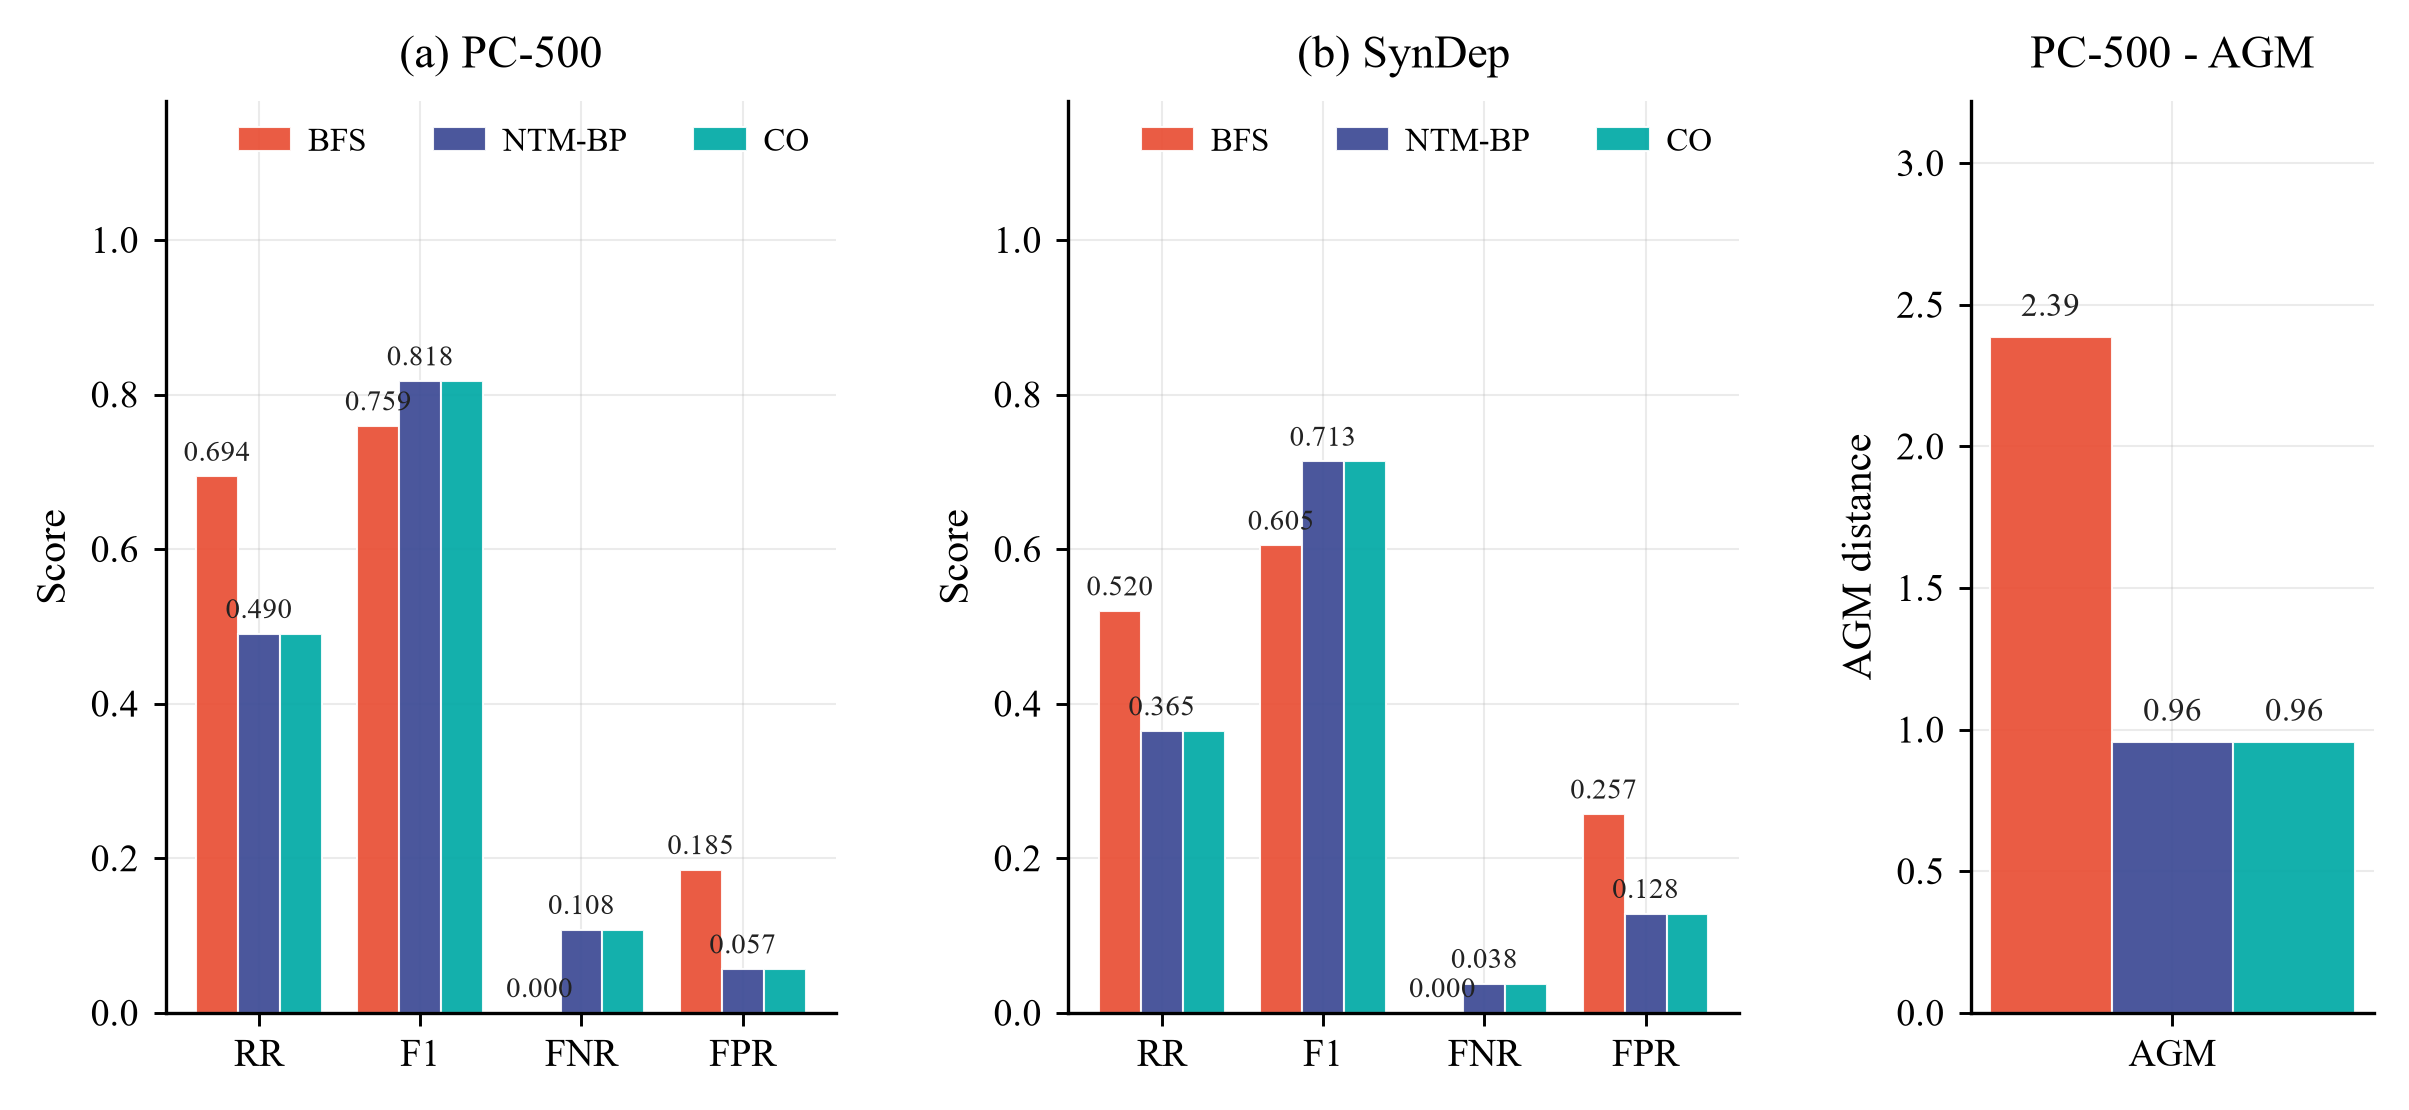
\includegraphics[width=0.95\linewidth]{figures/fig1_main_bar.png}
\caption{Algorithmic engine comparison on the full PC-500 (500
  instances) and SynDep (200 instances) sets: BFS, NTM-BP, and the CO
  extension across RR, F1, FNR, FPR, and AGM distance (rightmost
  panel, own scale).  Relation types are not annotated on these sets,
  so CO's edge-type multipliers are inert and CO coincides with
  NTM-BP; relation-aware CO variants are evaluated on
  relation-labeled chains (\cref{fig:relation-impact}), and the
  LLM-based gates on the sealed test sets
  (\cref{tab:sealed}).  Error bars denote $95\%$
  cluster-bootstrap confidence intervals ($2{,}000$ resamples).}
\label{fig:main-results}
\end{figure}

\subsection{Structured Semantic Gate}
\label{sec:structured}

While NTM-BP is zero-cost, its purely numeric nature means it cannot
distinguish between \emph{confirming} updates (``sales grew $5\%$''
when ``sales grew'' was already known) and \emph{truly neutral}
updates that should not trigger any re-evaluation chain.  The
Structured Semantic Gate addresses this by decomposing the gating
decision into three discrete, independently auditable LLM judgments.

\textbf{Decomposition.}  For each updated fact $f_k$ with old value
$v_{\text{old}}$ and new value $v_{\text{new}}$:

\begin{description}[style=nextline, leftmargin=1.8cm, labelwidth=1.5cm,
  labelsep=0.3cm, font=\normalfont\bfseries, itemsep=4pt, topsep=4pt]
\item[Q1---Change Type:] Is the update a directional
  change (A: negation, reversal, or the old trend no longer holds),
  a confirmation or reinforcement (B: same direction but stronger,
  reconfirmed, or superseded), or a minor fluctuation (C: isolated,
  episodic event that does not change the overall assessment)?
  Output: a single letter \texttt{A}, \texttt{B}, or \texttt{C}.

\item[Q2---Relevance:] Given the new situation
  $v_{\text{new}}$, would knowing it affect the judgment about a
  downstream conclusion $f_j$ (through direct or reasonable
  chain-of-consequence influence)?  Asked counterfactually:
  ``If this situation holds, would it affect the assessment of that
  conclusion?''  Output: \texttt{yes} or \texttt{no}.

\item[Q3---Stance:] When $\text{Q1}=\texttt{B}$
  (confirmation/reinforcement), does the new value align with or
  oppose the downstream conclusion?  \texttt{aligned}: the two are
  consistent or mutually reinforcing; \texttt{opposed}: conflict
  exists such that the new situation weakens the conclusion.
\end{description}

\textbf{Decision rule.}  A downstream conclusion $f_j$ is marked for
re-evaluation iff:
\begin{equation}
  \text{Q2}=\texttt{yes}\;\land\;\big(\text{Q1}=\texttt{A}\;\lor\;
  (\text{Q1}=\texttt{B}\;\land\;\text{Q3}=\texttt{opposed})\big).
  \label{eq:decision}
\end{equation}

\begin{figure}[t]
\centering
\providecolor{ntmblue}{HTML}{3B4994}
\providecolor{bforange}{HTML}{E94E34}
\begin{tikzpicture}[
  y=-1cm,
  box/.style={draw, rounded corners, align=center, inner sep=3pt,
              minimum height=8mm, font=\small},
  qbox/.style={box, fill=ntmblue!8, draw=ntmblue},
  stbox/.style={box, fill=ntmblue!18, draw=ntmblue, thick},
  skipbox/.style={box, fill=black!6, draw=black!60},
  markbox/.style={box, fill=bforange!16, draw=bforange, thick},
  keepbox/.style={box, fill=ntmblue!8, draw=ntmblue},
  dec/.style={draw, diamond, aspect=2.2, inner sep=1pt, align=center,
              font=\footnotesize, fill=black!4, draw=black!70},
  edge/.style={-{Stealth[length=2.2mm]}, draw=black!65},
  lbl/.style={font=\footnotesize, inner sep=1.5pt, fill=white},
]
\node[stbox]   (upd)  at (0,0)     {Fact update $f_k$: $v_{\mathrm{old}} \to v_{\mathrm{new}}$};
\node[qbox]    (q1)   at (0,1.2)   {\textbf{Q1} change type (1 call per update)};
\node[dec]     (dC)   at (0,2.6)   {Q1 = C?};
\node[skipbox] (skip) at (4.9,2.6) {Skip all targets\\(no further calls)};
\node[qbox]    (loop) at (0,4.0)   {for each downstream target $f_j$};
\node[qbox]    (q2)   at (0,5.3)   {\textbf{Q2} relevance (1 call per target)};
\node[dec]     (dQ2)  at (0,6.8)   {Q2 = yes?};
\node[keepbox] (keep) at (4.9,6.8) {Keep $f_j$};
\node[dec]     (dA)   at (0,8.4)   {Q1 = A?};
\node[qbox]    (q3)   at (4.9,8.4) {\textbf{Q3} stance (1 call per target)};
\node[markbox] (mark) at (0,10.0)  {Mark $f_j$ \texttt{REEVAL\_REQUIRED}};

\draw[edge] (upd)  -- (q1);
\draw[edge] (q1)   -- (dC);
\draw[edge] (dC)   -- node[lbl,above]{yes (Q1=C)} (skip);
\draw[edge] (dC)   -- node[lbl,right]{no} (loop);
\draw[edge] (loop) -- (q2);
\draw[edge] (q2)   -- (dQ2);
\draw[edge] (dQ2)  -- node[lbl,above]{no} (keep);
\draw[edge] (dQ2)  -- node[lbl,right]{yes} (dA);
\draw[edge] (dA)   -- node[lbl,above]{Q1=B} (q3);
\draw[edge] (dA)   -- node[lbl,right]{Q1=A} (mark);
\draw[edge] (q3)   -- node[lbl,right]{aligned} (keep);
\draw[edge] (q3.south) -- (q3.south |- mark.center)
                    -- node[lbl,below]{opposed} (mark.east);
\end{tikzpicture}
\caption{Decision flow of the Structured Semantic Gate.  Q1 is asked
  once per update; if \text{Q1}=$\texttt{C}$ all targets are skipped
  after this single call.  Otherwise, for each downstream target:
  Q2 (relevance) is asked first; on Q2=yes the Q1 verdict decides
  directly (A $\to$ mark), while for Q1=B a third call Q3 (stance)
  marks only opposed conclusions.  Every path thus takes the cheapest
  sufficient route.}
\label{fig:gate-flow}
\end{figure}

If $\text{Q1}=\texttt{C}$ (minor fluctuation), the engine returns
immediately after one LLM call per update---no downstream relevance or
stance calls are made (\cref{fig:gate-flow}).  This early-exit path is
the primary source of the structured gate's efficiency advantage.

\textbf{Design rationale.}  The three-way decomposition was motivated
by observing that a single scalar-prompt gate (our gate-v1 baseline)
exhibits a ``whac-a-mole'' dynamic during iterative development:
fixing missed opposed-conclusion updates would simultaneously cause
over-triggering on minor fluctuations, because the scalar must encode
change magnitude, semantic relevance, and directional stance in one
number.  Decoupling them allows each failure mode to be diagnosed and
addressed independently.  The counterfactual phrasing of Q2 avoids the
``already accounted for'' bias that plagued earlier prompt versions.

\textbf{Relationship between NTM-BP and the Structured Gate.}
The two mechanisms operate at different levels and are designed to be
complementary.  NTM-BP is a purely numeric engine: it propagates
confidence decay based on the source-change magnitude, edge conditional
probabilities, and the decay coefficient~$\gamma$, without any LLM
calls.  It handles the common case where a numeric confidence change
can be mechanically propagated through the dependency graph.  The
Structured Semantic Gate operates at the semantic level: it uses LLM
judgments to classify the update type, assess per-conclusion relevance,
and determine directional stance---dimensions that are orthogonal to
the numeric decay and cannot be captured by a single scalar score.
In practice, NTM-BP provides a zero-cost fallback with
F1 $=0.818$ on PC-500, while the structured gate adds
LLM-based semantic analysis for higher precision (F1 $=0.778$ on the
held-out expansion set) at a modest call cost (average 2.87 calls per
update).  The two can be deployed independently or combined: a
cost-sensitive system may use NTM-BP alone, routing to the structured
gate only for ambiguous update types (though we show in
\cref{sec:rq4} that naive type-based routing \emph{fails}).

% ======================================================================
\section{Theoretical Analysis}
\label{sec:theory}
% ======================================================================

\subsection{Cascade Completeness (Baseline)}

The BFS cascade is sound and linear-time: by standard BFS analysis
(each node and edge visited at most once), it marks every node
reachable from the updated source $v_k$ in $O(|V|+|E|)$ time, so no
downstream conclusion is missed---but all $|\text{Reach}(v_k)|$ nodes
are marked regardless of update magnitude, which is precisely the waste
NTM-BP removes.  (This is textbook BFS completeness, so we do not dress
it as a numbered theorem; the formal statement is in \cref{app:formal}.)

\subsection{NTM-BP Convergence on Trees}

\begin{theorem}[NTM-BP Convergence on Rooted Trees]
\label{thm:convergence}
If the dependency graph $G$ is a rooted tree (connected, acyclic, with
unique paths from root to all descendants), Algorithm~\ref{alg:ntmbp}
terminates after propagating at most $d$ hops from the updated source,
where $d$ is the maximum source-to-descendant path length.  The
converged belief for any node $f_j$ reachable from $f_k$ is:
\begin{equation}
  \mathcal{B}^*(f_j) = \mathcal{B}_0(f_j) \cdot
  \prod_{i=1}^{d}\Big(1 - \alpha\cdot\gamma^{i-1}\cdot
  \prod_{m=1}^{i}P_m\Big),
  \label{eq:converged}
\end{equation}
where $d$ is the path length from $f_k$ to $f_j$, and $P_m$ is the
conditional probability on the $m$-th edge of the path.
\end{theorem}

The result is a one-line consequence of the semi-group property of the
decay update ($\mathcal{B}_{t+1}=\mathcal{B}_t\times(1-\delta_{t+1})$
composing as a product along the unique root-to-node path on a tree);
the full proof sketch is given in \cref{app:formal}.

\begin{remark}[Loopy graphs: walk-sum view]
\label{rem:loopy}
Real dependency graphs are rarely trees (e.g., mutual reinforcement
between ``risk is manageable'' and ``supplier is reliable'').
Linearizing the update as $\mathbf{x}=\mathbf{b}+\gamma A\mathbf{x}$, the
walk-sum framework~\cite{malioutov2006walksum} gives a unique fixed
point whenever $\gamma\,\rho(A)<1$; on the DAGs we evaluate $A$ is
nilpotent ($\rho(A)=0$), so the condition holds trivially, and our
operating point $\gamma=0.7$ satisfies it for any
$\rho(A)<1/\gamma\approx1.428$.  We
verified this \emph{linearized} fixed-point iteration numerically on ring
and mutual-reinforcement graphs; the implemented Algorithm~\ref{alg:ntmbp}
uses a visited set and does not itself revisit nodes, so a formal proof
for the multiplicative (non-linearized) rule remains a conjecture left
to future work.  The spectral condition, the numerical protocol, and
the results are detailed in \cref{app:formal}.
\end{remark}

\subsection{Precision-Efficiency Tradeoff}

We characterize the tradeoff between re-evaluation rate (cost) and
accuracy (benefit) that NTM-BP achieves versus the binary cascade.

\begin{proposition}[Precision-Efficiency Tradeoff]
\label{thm:tradeoff}
Let a source update at $f_k$ change its confidence from
$\mathcal{B}_{\text{old}}$ to $\mathcal{B}_{\text{new}}$, producing a
normalized source change
$\alpha = \big(|\mathcal{B}_{\text{old}} - \mathcal{B}_{\text{new}}| /
\mathcal{B}_{\text{old}}\big) \big/ \big(\alpha_0 +
|\mathcal{B}_{\text{old}} - \mathcal{B}_{\text{new}}| /
\mathcal{B}_{\text{old}}\big)$.  For a downstream conclusion $f_j$ at
graph distance $d$ from $f_k$, with edge-wise CPT values
$P_1,\ldots,P_d$, the belief after NTM-BP propagation is:
\begin{equation}
  \mathcal{B}(f_j) = \mathcal{B}_0(f_j) \cdot
  \prod_{i=1}^{d}\Big(1 - \alpha\cdot\gamma^{i-1}\cdot
  \prod_{m=1}^{i}P_m\Big).
  \label{eq:belief-d}
\end{equation}
Let $\tau$ be the re-evaluation threshold.  Under the binary cascade,
$R_{\text{bin}}=1$ (the node is always marked).  Under NTM-BP,
$R_{\text{prob}} = \mathbb{I}[\mathcal{B}(f_j) < \tau]$, which depends
on $\alpha$, $d$, the CPT chain, and $\gamma$.  For deterministic
dependence (all $P_i=1$), every hop transmits the maximal decay
$\delta_i = \alpha\cdot\gamma^{i-1}$, so
$R_{\text{prob}} = \mathbb{I}[\mathcal{B}_0(f_j)\cdot
\prod_{i=1}^{d}(1-\alpha\cdot\gamma^{i-1}) < \tau]$; with a
substantial source change (e.g., $\alpha=0.85$, $\tau=0.7$) the
first hop drops belief to $0.15\cdot\mathcal{B}_0(f_j) < \tau$, so
$R_{\text{prob}}=R_{\text{bin}}=1$---deterministic dependencies are
always re-evaluated.  In the best case (weak dependence,
$P_i=P_{\min}>0$ with $\mathcal{B}_0(f_j)=1$), the condition for
$R_{\text{prob}}=0$ is:
\begin{equation}
  \prod_{i=1}^{d}\Big(1 - \alpha\cdot\gamma^{i-1}\cdot P_{\min}^{i}\Big)
  \geq \tau.
  \label{eq:retention-condition}
\end{equation}
\end{proposition}

\begin{proof}[Proof sketch]
\cref{eq:belief-d} follows directly from telescoping the recursive decay
rule in Algorithm~\ref{alg:ntmbp}: $\delta_1=\alpha P_1$ and
$\delta_i=\delta_{i-1}\gamma P_i$ give
$\delta_i=\alpha\gamma^{i-1}\prod_{m=1}^{i}P_m$, and the belief after $d$
hops is the product of the $(1-\delta_i)$ factors.  The deterministic-
and best-case claims follow by substituting $P_i=1$ and $P_i=P_{\min}$
respectively.  The full derivation and the empirical calibration against
the PC-500 results---including which CPT default ($0.5$ vs.\ $0.8$) is
used where---are given in \cref{app:formal}.
\hfill$\square$
\end{proof}

\subsection{Bounded Belief Perturbation}

NTM-BP also gives a quantitative \emph{bounded-perturbation} property
relative to AGM-style minimal change; we do not claim it solves the full
AGM minimal-change optimization problem.
Because the binary baseline zeroes every reachable belief while NTM-BP
only multiplies a positive belief by $(1-\delta_i)$ with
$\delta_i\in[0,1]$, NTM-BP never sets a belief below the binary value, so
the total perturbation is bounded by the baseline's:
\begin{equation}
  \sum_{f\in F}|\mathcal{B}_{\text{NTM}}(f)-\mathcal{B}'(f)|
  \leq \sum_{f\in F}|\mathcal{B}_{\text{bin}}(f)-\mathcal{B}'(f)|,
  \label{eq:agm}
\end{equation}
with strict inequality whenever any $\delta_i<1$ (the generic case).  This
is a one-line observation---multiplicative decay of a positive number
stays positive---rather than a deep result, so we state it inline; the
formal proposition and proof are in \cref{app:formal}.

% ======================================================================
\section{Experiments}
\label{sec:experiments}
% ======================================================================

We evaluate four methods---BFS cascade (binary baseline), NTM-BP
(numeric), gate-v1 (frozen scalar-prompt LLM gate), and the structured
gate (our method)---on three datasets under a strict held-out regime.
\emph{Naming convention:} ``gate-v1'' is the method name used in all
tables and figures (also called the ``scalar-prompt gate,'' or simply
the ``scalar gate,'' in prose; we write ``gate-v1'' rather than a bare
``v1'').  The single scalar prompt was itself refined over internal
rounds (v1$\to$v2$\to$v3) during development (\cref{sec:limitations});
all reported numbers use its \emph{final frozen} version, which keeps the
method name ``gate-v1'' to match the shipped cache and is denoted
\texttt{PROMPT\_BUILDERS[v1]} in the reproducibility package;
``CO'' always denotes the \emph{Co}-relation engine of
\cref{sec:rq4}---an optional, relation-aware extension of NTM-BP
that coincides with NTM-BP whenever edges carry no relation labels.
All LLM-based methods are \emph{frozen before test data generation or
annotation}; no prompt iteration touches the test cases.  Every LLM
call is recorded in a prompt-hash audit cache; evaluation scripts
refuse to overwrite existing results (one-shot).  Confidence intervals
use cluster bootstrap ($2{,}000$ resamples, seed $42$) resampling at
the $(\text{template\_id},\text{new\_value})$ case level.  Because the
sealed PC-500 and SynDep test sets are small ($n=9$ and $n=18$ cases),
their CIs are shown with only two decimal places for tabular
consistency and should be read as coarse intervals; the wider expansion-set CIs
($n=54$) are the more reliable precision indicators.

\textbf{Metrics.}  A method's \emph{re-evaluation set} $\hat{R}$ is the
set of conclusions it flags for re-evaluation given an update.
Comparing against the ground-truth set $R^*$ at the instance level, we
report F1 (the harmonic mean of precision and recall of $\hat{R}$
against $R^*$), the re-evaluation rate (RR $= |\hat{R}| / |\text{all
conclusions}|$, an expected-cost proxy), the false-negative rate
(FNR $=$ fraction of $R^*$ not flagged), and the false-positive rate
(FPR $=$ fraction of non-required conclusions incorrectly flagged).
\textbf{Evaluation unit.}  Every F1 in this paper is computed
\emph{per instance}---one update scored against the ground-truth
re-evaluation set $R^*$ of that instance---and then aggregated as an
\emph{unweighted (macro) mean} over instances; we do not pool
true/false positives globally before forming the ratio.  For the
expansion set, where 37 of 54 cases have $R^*=\emptyset$, an instance
whose correct answer is ``re-evaluate nothing'' is scored as a perfect
match (F1$=1$; we treat empty-set agreement as complete agreement) when
the method also returns the empty set, and these
empty-set matches enter the macro-average on the same footing as
non-empty cases.  The AGM
distance (\cref{fig:main-results}, rightmost panel) measures the
total belief change induced by an update,
$\text{AGM} = \sum_{f\in F}|\mathcal{B}(f)-\mathcal{B}'(f)|$
(\cref{eq:agm}); lower is better (closer to minimal change).

\textbf{Datasets.}
\textbf{PC-500.}  500 instances from 18 annotated cases (6 templates
$\times$ 3 update values), with per-instance confidence jitter
($\pm0.05$).  Template-level split yields a sealed test set of 9 cases
(249 jittered instances).  We distinguish the \emph{sealed} PC-500 split
(9 cases, used for final benchmarking, \cref{tab:sealed}) from the
\emph{full} PC-500 set (18 cases / 500 scenarios, used for exploratory
ablations and sensitivity analysis, \cref{tab:ablation-ntmbp,tab:gamma});
every table names the split it reports.  Ground-truth re-evaluation sets
are manually annotated algorithm-independently
(\cref{app:reproducibility}); the dual-annotator agreement ($\kappa=1.0$)
applies to the Expansion-500 held-out set described below.
\textbf{SynDep.}  30 annotated cases (10 templates $\times$ 3 update
values), 200 jittered instances, covering five topological patterns.
Template-level split yields 18 sealed test cases (120 instances).
\textbf{Expansion-500.}  A post-freeze held-out validation set of 54
never-seen cases ($\times 10$ jitter $= 540$ total), generated
\emph{after} all prompt iterations finished, inspired by
memory-benchmark methodologies~\cite{longmemeval,yushuai2025memorybench}.  Cases span 18 templates
across 12+ domains and five topologies.  The complete generation script,
the annotation sheets, and the resulting 540-instance dataset are included
in the reproducibility package (\cref{app:reproducibility}).
Two annotators (the author and a
blinded advisor, who filled a sheet with all labels
removed; \cref{app:reproducibility}) labeled
every case (Cohen's $\kappa=1.0$ at both the re-evaluation-set and
per-fact levels).  Of the 54 cases, 17 ($31\%$) have non-empty
ground-truth re-evaluation sets; the remaining 37 ($69\%$) require
zero re-evaluation.
\textbf{Expansion-Balanced.}  A second held-out set of 40 adversarial
cases balanced $20/20$ between non-empty and empty ground truth, designed
so that lexical and confidence cues are uninformative
(\cref{sec:balanced}).  Two annotators (the author and a blinded advisor)
labeled every case with perfect agreement ($\kappa=1.0$) at both the
case and per-fact levels.

We organize the experimental analysis around four questions:
\textbf{(RQ1)}~Is NTM effective?
\textbf{(RQ2)}~Why is it effective?
\textbf{(RQ3)}~Which components of the Structured Semantic Gate
contribute?
\textbf{(RQ4)}~Where does the method fail?

% -- RQ1 ----------------------------------------------------------------
\subsection{RQ1: Is NTM Effective?}
\label{sec:rq1}

\cref{tab:sealed} reports the sealed test results on PC-500 and
SynDep.

\begin{table}[t]
\centering
\caption{Sealed test results (one-shot, frozen prompts).  F1 scores
with $95\%$ cluster-bootstrap CIs ($2{,}000$ resamples).}
\label{tab:sealed}
\begin{tabular}{lcc}
\toprule
Method & PC-500 (9 cases) & SynDep (18 cases) \\
\midrule
BFS (binary cascade)        & $0.854$ [$0.63$, $1.00$] & $0.626$ [$0.40$, $0.83$] \\
NTM-BP (numeric)            & $0.851$ [$0.72$, $0.96$] & $0.703$ [$0.51$, $0.86$] \\
gate-v1 (frozen scalar)     & $0.854$ [$0.63$, $1.00$] & $0.692$ [$0.48$, $0.88$] \\
\textbf{Structured (ours)}  & $\mathbf{0.854}$ [$0.63$, $1.00$] &
                              $\mathbf{0.807}$ [$0.63$, $0.96$] \\
\bottomrule
\end{tabular}
\end{table}

On PC-500 the sealed split is saturated: all methods, including the
binary BFS cascade, tie at approximately $0.85$ F1, because in almost
every selected case the ground-truth re-evaluation set equals the full
downstream set, so binary and selective propagation agree.  On SynDep,
the structured gate leads by $+10.4$ points over NTM-BP ($0.807$ vs.\
$0.703$) and $+11.5$ over gate-v1 ($0.807$ vs.\ $0.692$); note that on
this split BFS ($0.626$) is clearly below the selective methods.

\cref{tab:expansion} reports the held-out validation on the 54
never-seen expansion cases.

\begin{table}[t]
\centering
\caption{Expansion-500 held-out validation (54 cases, 540 instances,
  dual-annotator labels, frozen methods).}
\label{tab:expansion}
\begin{tabular}{lc}
\toprule
Method & F1 \\
\midrule
BFS (binary cascade)        & $0.315$ [$0.19$, $0.44$] \\
NTM-BP (numeric)            & $0.686$ [$0.60$, $0.76$] \\
gate-v1 (frozen scalar)     & $0.667$ [$0.54$, $0.78$] \\
\textbf{Structured (ours)}  & $\mathbf{0.778}$ [$0.67$, $0.89$] \\
\bottomrule
\end{tabular}
\end{table}

The structured gate achieves the highest point estimate, leading by
$0.092$ F1 ($9.2$ percentage points) over NTM-BP and $0.111$ ($11.1$
percentage points) over gate-v1.  A paired cluster-bootstrap (instances
nested within the 54 cases) finds the structured-vs-BFS difference
($0.463$ F1, $46.3$ percentage points) significant ($p<0.001$), but the
differences over NTM-BP ($0.092$ F1, $p=0.18$) and over gate-v1
($0.111$ F1, $p=0.14$) are \emph{not} significant at
$\alpha=0.05$ with only 54 cases; we therefore do not claim that the
structured gate significantly outperforms NTM-BP on this benchmark.
\emph{Multiple comparisons.}  We report three pairwise tests against
the structured gate (vs.\ BFS, vs.\ NTM-BP, vs.\ gate-v1); a
Holm--Bonferroni correction across these three comparisons leaves
structured-vs-BFS significant (adjusted $p<0.003$) and does not change
the non-significance of the NTM-BP and gate-v1 comparisons, so no claim in
this paper rests on an uncorrected $p$-value.

\textbf{Stratified analysis: lexically marked vs.\ unmarked (post-hoc).}
This split is an \emph{exploratory, post-hoc} analysis: the
marked/unmarked stratification was defined \emph{after} observing the
structured gate's per-subset performance, so \cref{tab:stratified} is
hypothesis-generating rather than a pre-registered confirmatory test,
and its subset-level differences inherit the same small-sample caveats
as the overall comparison.  To understand when each method succeeds, we
stratify the 54 cases by whether the new fact value contains an overt
negative lexical cue (e.g., ``deteriorated,'' ``declined,''
``strike'').  Of 54 cases, 22 are lexically marked and 32 are unmarked.
\cref{tab:stratified} reports the results.

\begin{table}[t]
\centering
\caption{Stratified F1 on Expansion-500 by lexical marking.  The
  unmarked split is dominated by empty ground truth ($31$ of $32$ cases),
  so that column mainly reflects over-trigger behaviour; the keyword
  baselines are overall-only and unstratified (\cref{sec:rq4}).}
\label{tab:stratified}
\begin{tabular}{lcc}
\toprule
Method & Marked (22) & Unmarked (32) \\
\midrule
BFS (binary cascade)        & $0.727$ & $0.031$ \\
NTM-BP (numeric)            & $0.771$ & $0.628$ \\
gate-v1 (frozen scalar)     & $0.955$ & $0.469$ \\
\textbf{Structured (ours)}  & $0.909$ & $\mathbf{0.688}$ \\
\midrule
\multicolumn{3}{l}{\emph{Overall-only lexical baselines (not stratified)}} \\
Keyword (text match)        & \multicolumn{2}{c}{$0.833$ (overall)} \\
Keyword+Confidence          & \multicolumn{2}{c}{$0.944$ (overall)} \\
\bottomrule
\end{tabular}
\end{table}

On lexically marked cases, the scalar gate achieves the highest F1
($0.955$), and the structured gate ($0.909$) and keyword baseline
($0.833$) also perform well.  The unmarked column, however, must be read
with care: $31$ of its $32$ cases have empty ground truth, so any
conservative method scores highly there, and the zero-cost keyword rule
(not stratified in this table) in fact reaches F1 $=1.0$ on that subset
(it correctly skips the $31$ empty cases and fires on the single
non-empty one), above the structured gate's $0.688$; a paired test on the
$32$ unmarked cases favors the rule ($\Delta=+0.313$, $p<0.001$,
post-hoc; \cref{sec:rq4}).  We therefore do \emph{not} read the unmarked
subset as evidence that the gate handles unmarked changes better than
cheaper rules.  The structured gate's advantage over the \emph{scalar}
baseline on this subset ($\Delta$F1 $=0.219$, $p=0.037$) and its
non-significance versus NTM-BP ($\Delta$F1 $=0.060$, $p=0.57$) are
reported as hypothesis-generating; the regime in which the gate's
semantic decomposition does add measurable value is the balanced
adversarial set of \cref{sec:balanced}.

\textbf{Non-empty vs.\ empty case breakdown.}
Of 54 cases, 17 require re-evaluation (non-empty ground truth) and 37
require none (empty).  On the 170 non-empty instances, BFS, scalar gate,
and structured gate all achieve perfect F1 ($1.000$); NTM-BP scores
$0.909$.  On the 370 empty instances (accuracy = correctly skipping), BFS
achieves $0.000$ (it re-evaluates everything, so it correctly skips
none), NTM-BP $0.584$, scalar gate $0.514$, and the structured gate
$0.676$---the highest of the non-trivial methods.  These two subsets
reproduce the macro-averaged F1 of \cref{tab:expansion}: for the
structured gate, $(170\times1.000+370\times0.676)/540=0.778$.  The
structured gate thus skips more empty cases than either NTM-BP or the
scalar gate; its residual over-trigger rate is confined to borderline
semantic changes, the price of the sensitivity that the balanced set of
\cref{sec:balanced} shows is useful when cues are absent.

\textbf{NTM-BP component ablation.}
\cref{tab:ablation-ntmbp} shows the contribution of the propagation
decay $\gamma$ versus the binary cascade (\cref{fig:ablation-components}).

\begin{table}[t]
\centering
\caption{NTM-BP component ablation on full PC-500 (500 scenarios).}
\label{tab:ablation-ntmbp}
\begin{tabular}{lcccc}
\toprule
Variant & F1 & RR & FNR & FPR \\
\midrule
BFS (binary cascade)            & $0.759$ & $0.694$ & $0.000$ & $0.185$ \\
NTM-BP ($\gamma=0.7$)          & $0.818$ & $0.491$ & $0.108$ & $0.057$ \\
NTM-BP ($\gamma=1.0$, no decay) & $0.876$ & $0.569$ & $0.005$ & $0.065$ \\
\bottomrule
\end{tabular}
\end{table}

NTM-BP with $\gamma=0.7$ reduces the re-evaluation rate by $29.3\%$
relative to BFS (RR $0.491$ vs.\ $0.694$) while maintaining F1 above
$0.80$.  Removing the propagation decay ($\gamma=1.0$) raises F1 to
$0.876$ but increases RR to $0.569$---effectively reverting toward the
BFS extreme.  The near-zero FNR of $\gamma=1.0$ ($0.005$) confirms that
propagation without decay is essentially the binary cascade with softer
thresholds.

\textbf{Summary.}  NTM is effective: the structured gate achieves
F1 $=0.778$ on the held-out expansion set (vs.\ BFS $0.315$), and NTM-BP alone
reduces the re-evaluation rate by $29.3\%$ while maintaining F1 $=0.818$
on the full PC-500 set.  The decay coefficient $\gamma$ is the
primary driver of the F1-RR tradeoff.

% -- Balanced adversarial held-out set ----------------------------------
\subsection{Balanced Adversarial Held-out Set}
\label{sec:balanced}

The Expansion-500 distribution is $37/54$ empty, so its macro-F1 mostly
rewards correctly skipping.  To test discrimination in the opposite
regime we constructed a second held-out set, \textsc{Expansion-Balanced},
of $40$ cases balanced $20/20$ between non-empty and empty ground truth
and designed to separate \emph{semantic} relevance from \emph{lexical}
and \emph{numeric} signals.  The non-empty cases mostly use neutral
surface wording with only a small confidence change---so neither a
negative keyword nor a confidence-drop threshold can detect them---while
the empty cases deliberately include negative-sounding wording, large
confidence drops, and strengthening (supersede-style) updates.  Labels
were produced by the same written policy as Expansion-500
(\cref{app:reproducibility}); two annotators (the author and a blinded
advisor) labeled every case with perfect agreement ($\kappa=1.0$) at both
the case and per-fact levels.  \cref{tab:balanced} reports the
results.

\begin{table}[t]
\centering
\caption{\textsc{Expansion-Balanced} held-out results ($40$ cases:
  $20$ non-empty / $20$ empty).  ``Macro'' is the unweighted
  instance-level macro mean; because the set is balanced, macro and
  skip-balanced F1 coincide.  Labels: dual-annotator, $\kappa=1.0$.}
\label{tab:balanced}
\begin{tabular}{lccc}
\toprule
Method & Non-empty F1 & Empty F1 & Macro F1 \\
\midrule
BFS (binary cascade)        & $1.000$ & $0.000$ & $0.500$ \\
NTM-BP (numeric)            & $0.880$ & $0.850$ & $0.865$ \\
gate-v1 (frozen scalar)     & $1.000$ & $0.750$ & $0.875$ \\
\textbf{Structured (ours)}  & $\mathbf{1.000}$ & $\mathbf{0.950}$ & $\mathbf{0.975}$ \\
\texttt{kw\_text\_conf} (zero-cost)  & $0.650$ & $0.800$ & $0.725$ \\
\bottomrule
\end{tabular}
\end{table}

On this balanced set the structured gate attains the highest F1
($0.975$), significantly above NTM-BP (paired $\Delta=+0.110$, $95\%$
CI $[0.045,0.188]$, $p<0.001$) and the zero-cost keyword rule
($\Delta=+0.250$, CI $[0.10,0.40]$, $p=0.001$), though not significantly
above the scalar gate-v1 ($\Delta=+0.100$, $p=0.13$).  The keyword rule's
F1 falls to $0.725$: because the high-impact updates carry no overt
negative cue and little confidence change, the rule misses them
(non-empty F1 $0.65$), while it over-fires on negative-sounding but
immaterial updates (empty F1 $0.80$).  This is the regime in which the
structured gate's semantic decomposition adds measurable value; on the
original Expansion-500 distribution, by contrast, the impact signal is
largely lexically marked and the rule dominates (\cref{sec:rq4}).  We
report both regimes side by side rather than the more favorable one
alone.

% -- RQ2 ----------------------------------------------------------------
\subsection{RQ2: Why Is NTM Effective?}
\label{sec:rq2}

The dependence of re-evaluation rate on the magnitude of the source
update, which motivates the entire framework, is illustrated in
\cref{fig:rr-theta}: BFS maintains a flat, relatively high RR regardless of
$\theta$, whereas NTM-BP tracks the impact magnitude;
\cref{fig:belief-network} visualizes the resulting belief states on a
small graph.

\begin{figure}[t]
\centering
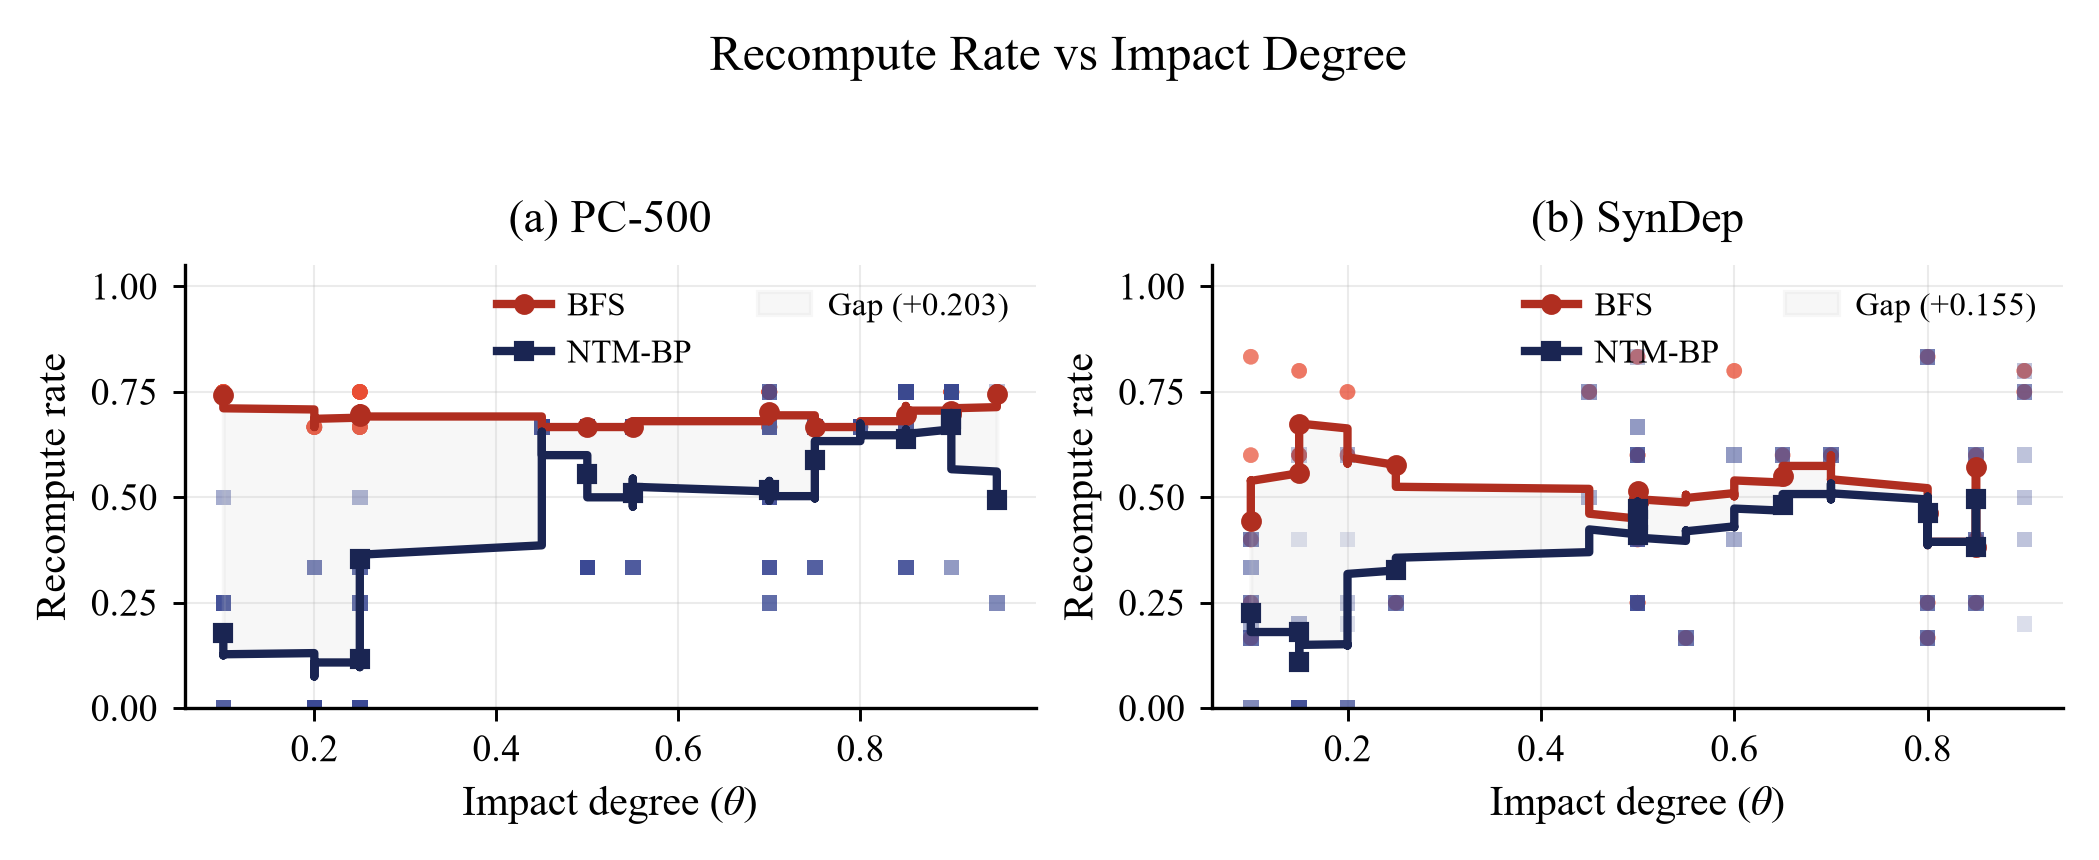
\includegraphics[width=0.95\linewidth]{figures/fig2_rr_vs_theta.png}
\caption{Recompute rate as a function of source-impact degree $\theta$
  on PC-500 and SynDep.  BFS maintains a flat, relatively high RR regardless
  of $\theta$; NTM-BP tracks the impact magnitude.  CO coincides with
  NTM-BP on these sets (relation types are not annotated), so only
  NTM-BP is shown.}
\label{fig:rr-theta}
\end{figure}

\textbf{Per-case win/loss analysis (structured vs.\ NTM-BP).}  Out of
54 expansion cases: win 20, lose 9, tie 25.  Of the 20 wins, 11 are
type-C (minor fluctuation) cases where the structured gate's Q1
early-exit (C$\to$skip) correctly returns after one LLM call while
NTM-BP's numeric decay over-triggers; the remaining 9 wins are split
across type-A (7) and type-B (2) cases where the relevance path beats
numeric decay.  This confirms that the structured gate's primary
advantage is its ability to \emph{skip} irrelevant minor-fluctuation
updates that numeric decay cannot distinguish from genuine changes.

\textbf{Gamma sensitivity.}
\cref{tab:gamma} reports the effect of varying $\gamma$ on PC-500.

\begin{table}[t]
\centering
\caption{Gamma sensitivity on PC-500 (500 scenarios).  $\Delta$F1 is
  the paired bootstrap mean difference vs.\ $\gamma=1.0$, with $95\%$
  CI.  $*$ denotes significance at $p<0.05$.}
\label{tab:gamma}
\begin{tabular}{lcccc}
\toprule
$\gamma$ & F1 & RR & $\Delta$F1 vs.\ no-decay & Significant? \\
\midrule
$0.5$        & $0.759$ & $0.421$ & $-0.117$ [$-0.188$, $-0.043$] & $*$ \\
$0.6$        & $0.787$ & $0.456$ & $-0.088$ [$-0.146$, $-0.031$] & $*$ \\
$0.7$        & $0.818$ & $0.491$ & $-0.059$ [$-0.098$, $-0.017$] & $*$ \\
$0.8$        & $0.848$ & $0.526$ & $-0.028$ [$-0.054$, $-0.004$] & $*$ \\
$0.9$        & $0.871$ & $0.558$ & $-0.005$ [$-0.013$, $+0.003$] & no \\
$1.0$ (no decay) & $0.876$ & $0.569$ & --- (baseline) & --- \\
\bottomrule
\end{tabular}
\end{table}

\begin{figure}[t]
\centering
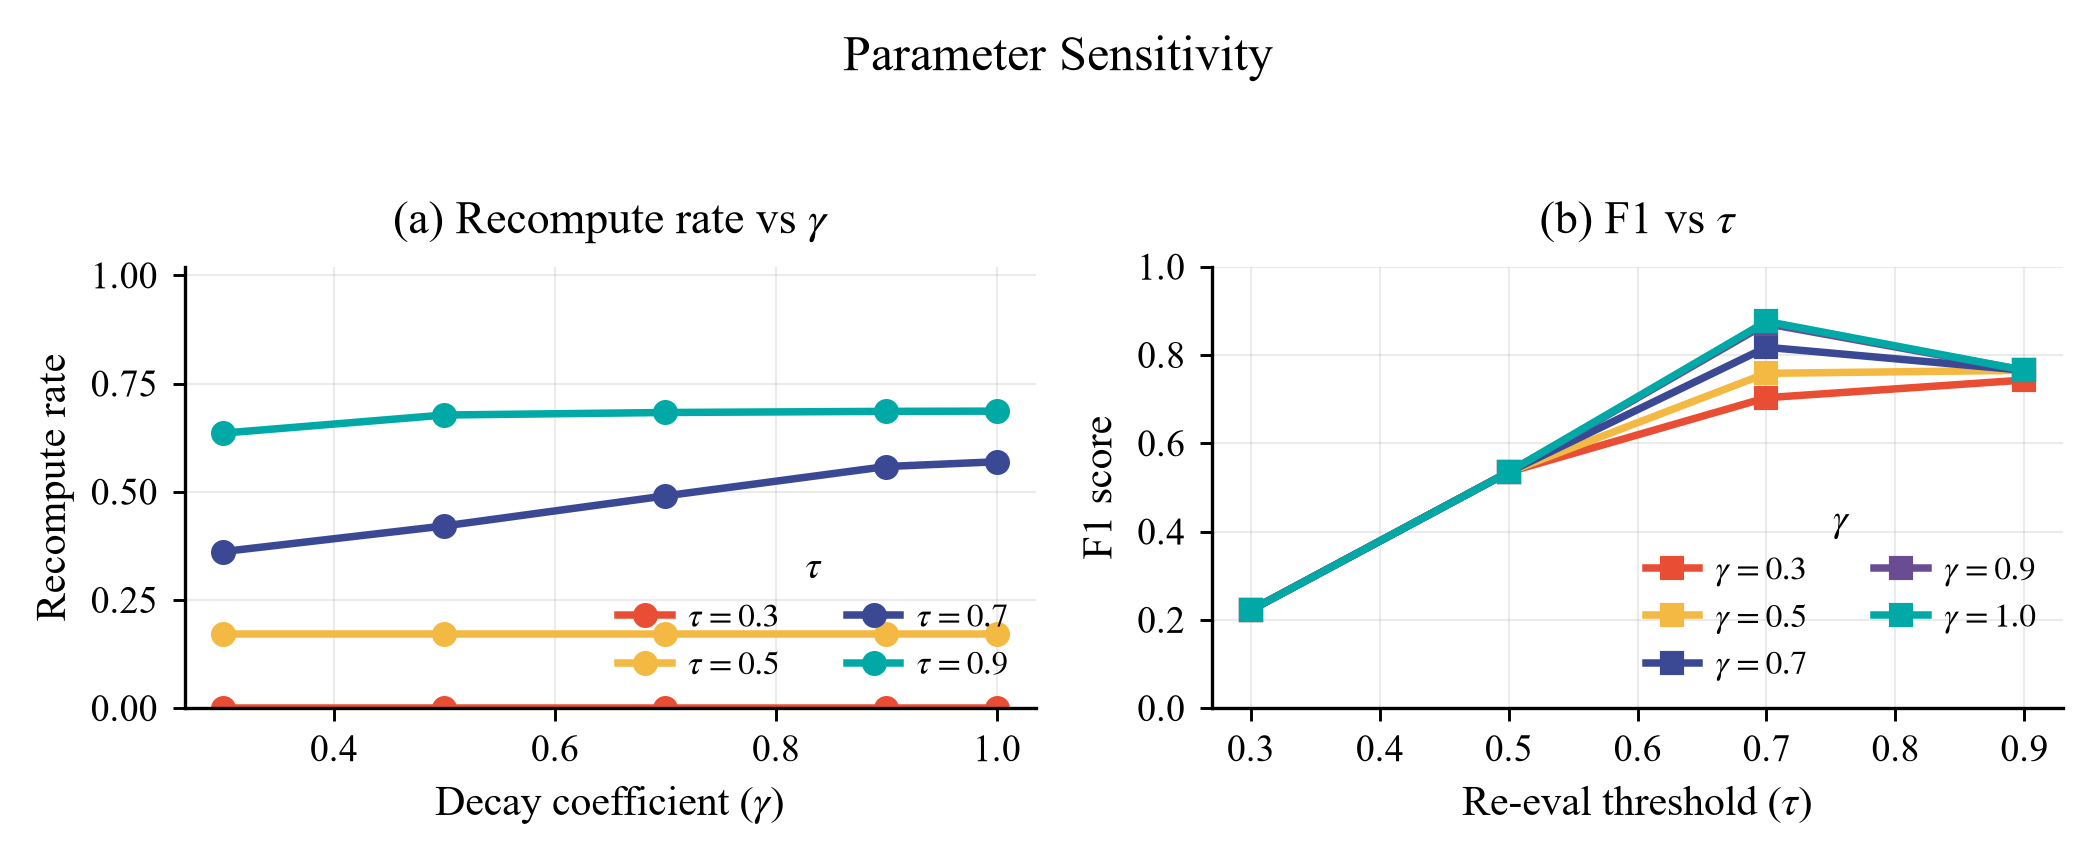
\includegraphics[width=0.95\linewidth]{figures/fig4_param_curves.png}
\caption{Parameter sensitivity: \textbf{(left)} $\gamma$ vs.\ RR across
  multiple $\tau$ settings; \textbf{(right)} $\tau$ vs.\ F1 across
  multiple $\gamma$ settings.}
\label{fig:param-curves}
\end{figure}

The decay coefficient $\gamma$ exerts smooth, monotonic control over the
F1-RR tradeoff.  Paired differences are statistically significant for
$\gamma\leq 0.8$, indicating that the effect of decay is distinguishable from
noise.  \cref{fig:param-curves,fig:heatmap} show the corresponding
$\gamma$--$\tau$ sensitivity surfaces.

\textbf{Scalability.}
\cref{tab:scalability} reports wall-clock latency per update, with the
scaling curves in \cref{fig:scalability,fig:scalability-rr}.

\begin{table}[t]
\centering
\caption{Per-update wall-clock latency (ms) vs.\ graph size.
  Measured with the original research build on Python 3.11 / Intel
  i7-12700H; absolute latencies are hardware- and implementation-specific.
  \texttt{scripts/experiment\_scalability\_latency.py} benchmarks the
  shipped dependency-free port.}
\label{tab:scalability}
\begin{tabular}{lrrrrrr}
\toprule
Method & 10 & 50 & 100 & 200 & 500 & 1{,}000 \\
\midrule
BFS (binary)   & $0.24$ & $0.75$ & $1.29$ & $3.76$ & $7.52$  & $17.57$ \\
NTM-BP         & $0.24$ & $0.79$ & $1.85$ & $3.29$ & $10.79$ & $18.42$ \\
CO (relation)  & $0.18$ & $0.48$ & $1.58$ & $4.05$ & $7.31$  & $17.64$ \\
\bottomrule
\end{tabular}
\end{table}

All methods complete within $20$~ms even on $1{,}000$-node graphs,
roughly $25$--$100\times$ faster than a single LLM inference
call ($\sim 500$--$2{,}000$~ms).

\textbf{Robustness to CPT perturbation.}
\cref{tab:cpt-noise} shows that F1 is essentially flat across the entire
noise range ($\Delta\mathrm{F1}\le 0.006$).  The engine's decisions are
driven primarily by the source-change ratio and the $\gamma$-attenuated
hop structure rather than by the precise edge probabilities.

\begin{table}[t]
\centering
\caption{NTM-BP F1 on PC-500 under CPT perturbation
  ($P=0.8+\mathcal{N}(0,\sigma^2)$, 10 seeds).}
\label{tab:cpt-noise}
\begin{tabular}{lccccc}
\toprule
$\sigma$ & $0$ & $0.05$ & $0.10$ & $0.15$ & $0.20$ \\
\midrule
F1 & $0.819$ & $0.822{\scriptstyle\pm.003}$ & $0.822{\scriptstyle\pm.003}$
   & $0.824{\scriptstyle\pm.005}$ & $0.822{\scriptstyle\pm.005}$ \\
\bottomrule
\end{tabular}
\end{table}

% -- RQ3 ----------------------------------------------------------------
\subsection{RQ3: Which Structured Gate Components Contribute?}
\label{sec:rq3}

\cref{tab:ablation} compares the full structured gate with ablated
variants, replayed offline from the frozen prompt cache on the SynDep
development and sealed-test splits.

\begin{table}[t]
\centering
\caption{Structured-gate component ablation on SynDep, replayed offline
from the frozen prompt cache.  The sub-questions are only partially
independent: removing Q3 or replacing the binary relevance judgment with a
scalar costs at most $0.7$ points on the sealed test, and raises F1 on the
development split.}
\label{tab:ablation}
\begin{tabular}{lcc}
\toprule
Variant & Dev F1 & Test F1 \\
\midrule
Full structured gate (final)                    & $0.735$ & $\mathbf{0.807}$ \\
\quad-- Q3 stance removed (B always skips)      & $0.823$ & $0.807$ \\
\quad-- Q2 relevance replaced with scalar       & $0.823$ & $0.800$ \\
Scalar-prompt baseline (gate-v1)                & $0.520$ & $0.692$ \\
\bottomrule
\end{tabular}
\end{table}

On the sealed test the structured gate reaches $0.807$ versus $0.692$ for
the scalar-prompt baseline ($+11.5$ points), and the dev-to-test check
confirms no leakage (the full gate improves from $0.735$ on the dev set to
$0.807$ on the held-out test set).  The per-component ablation, however,
does \emph{not} show that each sub-question contributes a measurable
accuracy gain: removing Q3 (B always skips) leaves the test F1 unchanged
($0.807$), replacing the binary relevance judgment with a scalar impact
score costs only $0.7$ points ($0.800$), and on the development split
removing either \emph{raises} F1 ($0.735\to 0.823$), i.e., the stance and
relevance sub-questions are partially redundant on this distribution and
can also over-fire.  We therefore attribute the decomposition's measured
advantage to the joint three-question design---which beats the scalar
baseline---rather than to the marginal value of any single sub-question,
and rely on the early-exit cost saving (\cref{sec:rq2}) and the
auditability of the logged sub-answers as the operational benefits.

% -- RQ4 ----------------------------------------------------------------
\subsection{RQ4: Where Does the Method Fail?}
\label{sec:rq4}

\textbf{Failure mode 1: Supersede-strengthening misclassification.}
All 9 losses relative to NTM-BP are over-triggering cases in which Q1
returns type-A.  Most are \emph{supersede-strengthening} updates---e.g.,
``on-time rate hits an all-time high'', ``bumper harvest ahead'',
``additional spectrum approved'', ``full regression passed'', ``perfect
score from students'', ``third-party re-inspection all clear'', ``new
school construction begins''---where Q1 misreads supersession as a
directional change: ``all-time high'' and ``perfect score'' imply the
old state has been \emph{superseded}, which the LLM reads as ``the old
state no longer holds''.  The remaining two losses are other
over-inclusions of class A---a minor single-week dip and a branch-layout
adjustment---whose downstream conclusions the annotators judged
unaffected.  In all cases the structured gate then proceeds down the full
relevance path, falsely triggering whole-chain re-evaluation.  NTM-BP avoids these errors
because its numeric decay is insensitive to semantic framing: a
strengthening update with
$P(\text{child}\mid\text{parent})\approx1.0$ produces near-zero decay
and correctly bypasses re-evaluation.

We probed whether this is a \emph{general LLM tendency} (treating
supersession as negation) by re-running the frozen Q1 prompt under the
reasoning mode of the same model (\texttt{deepseek-reasoner}; an auxiliary
diagnostic whose raw responses are not part of the shipped cache).  On the
10 empty-ground-truth cases labelled type-A by the non-thinking mode
(\texttt{deepseek-chat}), the reasoning mode
agrees on only 4 and reclassifies 6 as B or C ($42/54$ overall Q1
agreement); these 10 cases are the 9 relative losses plus one in which
NTM-BP over-triggers identically.  The failure is therefore
\emph{partially} shared across inference modes but is not universal: it is
a tendency we observe for this model and prompt pair---a stronger
reasoning mode reduces it but does not eliminate it---and we do not
claim it generalizes beyond these ten cases and this provider.
The frozen scalar-prompt gate (gate-v1), using the same
\texttt{deepseek-chat} model as the structured gate, also fails on 7 of
the 9 cases (F1$=0.0$), which is consistent with a model/prompt-specific
rather than decomposition-specific cause.

\textbf{Failure mode 2: Keyword baseline outperforms the structured
gate.}
\cref{tab:kwbaseline} reveals that a purely lexical rule augmented with
the numeric confidence signal (\texttt{kw\_text\_conf}) reaches F1
$=0.944$ at zero LLM cost, \emph{above} the structured gate's $0.778$
on the expansion set.

\begin{table}[t]
\centering
\caption{Zero-cost keyword baselines on Expansion-500 (540 instances,
  cluster bootstrap CI).  All baselines make no LLM calls.}
\label{tab:kwbaseline}
\begin{tabular}{lcc}
\toprule
Baseline & F1 & Re-eval rate \\
\midrule
Always skip                    & $0.685$ [$0.57$, $0.80$] & $0.000$ \\
\texttt{kw\_text}              & $0.833$ [$0.72$, $0.93$] & $0.213$ \\
\texttt{kw\_negation}          & $0.852$ [$0.76$, $0.94$] & $0.231$ \\
\texttt{kw\_text\_conf}        & $0.944$ [$0.87$, $1.00$] & $0.333$ \\
BFS (binary, all downstream)   & $0.315$ [$0.19$, $0.44$] & $0.889$ \\
\bottomrule
\end{tabular}
\end{table}

We read the keyword result as a \emph{distributional boundary condition}
rather than a refutation.  On Expansion-500 the high-impact updates are
lexically marked (``worsened'', ``ambiguity'', ``missed endpoint''), so a
rule that sees both the text and the confidence delta has little left to
infer: a paired cluster bootstrap confirms that \texttt{kw\_text\_conf}
significantly \emph{outperforms} the structured gate on this set
($\Delta=+0.167$ F1, $95\%$ CI $[0.05,0.29]$, $p<0.001$).  The
structured gate's value is therefore \emph{not} established on this
distribution.  Two caveats sharpen what that means.  First, the set is
skip-dominated ($37/54$ empty), and of the $32$ ``unmarked'' cases $31$
have empty ground truth, so any conservative method scores well there; a
paired test on that subset also favors the rule ($\Delta=+0.313$,
$p<0.001$).  Second, the rule's advantage depends on the impact signal
being carried by lexical cues and confidence drops, which need not hold
in general: on the balanced adversarial set of \cref{sec:balanced},
where those cues are absent by construction, the rule falls to F1
$0.725$ and is significantly worse than the structured gate
($\Delta=-0.250$, $p=0.001$).  The gate's distinctive contributions---%
semantic relevance where cues are absent, and an auditable, decomposed
decision whose sub-answers can be logged and contested---are thus real
but conditional, and we do not claim them on Expansion-500.

The same zero-cost rule is also competitive on the sealed test sets
(\cref{tab:kwsealed}): \texttt{kw\_text\_conf} matches or beats the
structured gate on both (F1 $0.963$ vs.\ $0.854$ on PC-500; $0.851$
vs.\ $0.807$ on SynDep) at zero LLM cost.  The boundary condition is
therefore not specific to Expansion-500: whenever impact-bearing updates
carry overt negative cues, a keyword-plus-confidence rule is hard to
beat, and the gate's value is confined to update regimes where such
cues are absent or misleading, and to auditability.

\begin{table}[t]
\centering
\caption{Zero-cost keyword baselines on the sealed PC-500 and SynDep test
  sets (F1).  The split is the same as \cref{tab:sealed} and was not used
  for prompt tuning; \texttt{kw\_text\_conf} triggers on a negative
  keyword or a $\ge0.30$ confidence drop.}
\label{tab:kwsealed}
\begin{tabular}{lcc}
\toprule
Method & PC-500 (9 cases) & SynDep (18 cases) \\
\midrule
\texttt{kw\_text}       & $0.333$ & $0.386$ \\
\texttt{kw\_text\_conf} & $\mathbf{0.963}$ & $\mathbf{0.851}$ \\
BFS (binary)            & $0.854$ & $0.626$ \\
Structured gate (ours)  & $0.854$ & $0.807$ \\
NTM-BP                  & $0.851$ & $0.703$ \\
\bottomrule
\end{tabular}
\end{table}

\begin{figure}[t]
\centering
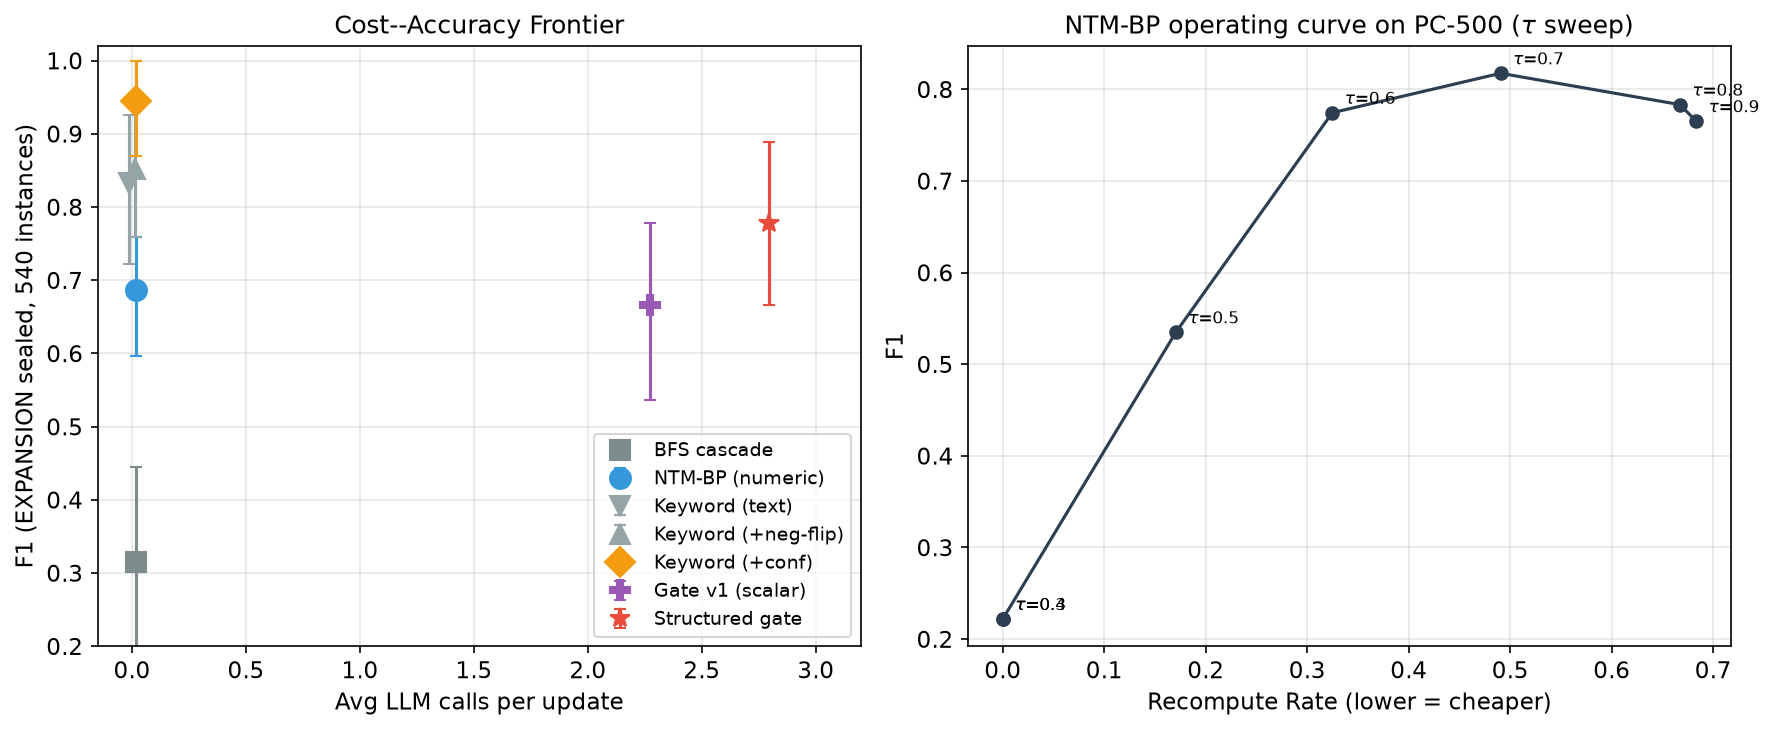
\includegraphics[width=\linewidth]{figures/pareto_cost_accuracy.png}
\caption{Cost--accuracy frontier.  \emph{Left}: F1 vs.\ average LLM
  calls per update on the held-out expansion set.  \emph{Right}: the
  tunable operating curve of NTM-BP on PC-500 obtained by sweeping
  $\tau$.}
\label{fig:pareto}
\end{figure}

\textbf{Failure mode 3: Naive type-based routing.}
\cref{tab:routing} shows that a naive routing strategy (B$\to$NTM-BP,
A$\to$LLM) \emph{fails}: F1 drops from $0.778$ to $0.750$.  The routing
rule was frozen only after the results motivating it were observed, so
this is an exploratory post-hoc simulation (replayed from the frozen
cache, zero new API calls); it is reported here only as a negative result
and never as an ex-ante routing evaluation.

\begin{table}[t]
\centering
\caption{Routing v0 post-hoc simulation on Expansion-500 (cache replay,
  zero new API calls).  \emph{NOT} ex-ante; reported as a negative
  result.}
\label{tab:routing}
\begin{tabular}{lcc}
\toprule
Method & F1 & LLM calls / update \\
\midrule
BFS (binary)         & $0.315$ & $0.0$ \\
NTM-BP (numeric)     & $0.686$ & $0.0$ \\
gate-v1              & $0.667$ & $2.28$ \\
Structured (ours)    & $\mathbf{0.778}$ & $2.87$ \\
Routing v0 (naive)   & $0.750$ & $2.24$ \\
\bottomrule
\end{tabular}
\end{table}

All five routing losses occur on Q1$\to$B cases where the numeric path
underperforms the structured stance path---NTM-BP cannot distinguish
``confirmed and settled'' from ``confirmed and still moving''.
This negative result bounds what pure routing can achieve without
fixing the underlying Q1 supersede-classification problem.

\textbf{CO engine: relation-aware propagation.}
The CO engine extends NTM-BP with edge-type multipliers
(\texttt{supports} $\times 1.2$, \texttt{contradicts} $\times 1.3$,
\texttt{neutral} $\times 0.5$).

\begin{table}[t]
\centering
\caption{CO engine vs.\ NTM-BP per relation type (500 scenarios each,
  oracle labels).}
\label{tab:co}
\begin{tabular}{lcccc}
\toprule
Method / Relation & F1 & RR & FNR & FPR \\
\midrule
NTM-BP (uniform)      & $0.818$ & $0.491$ & $0.108$ & $0.057$ \\
CO \texttt{supports}   & $0.857$ & $0.543$ & $0.038$ & $0.061$ \\
CO \texttt{contradicts}& $0.873$ & $0.560$ & $0.014$ & $0.062$ \\
CO \texttt{neutral}    & $0.709$ & $0.371$ & $0.275$ & $0.053$ \\
CO \texttt{mixed}      & $0.813$ & $0.485$ & $0.116$ & $0.058$ \\
\bottomrule
\end{tabular}
\end{table}

CO outperforms on \texttt{supports} ($+3.9$ F1) and
\texttt{contradicts} ($+5.5$ F1) but underperforms on \texttt{neutral}
($-10.9$ F1), reflecting a tension between sensitivity and specificity
(\cref{tab:co}).
CO is positioned as an optional extension, not a core component.

\begin{figure}[t]
\centering
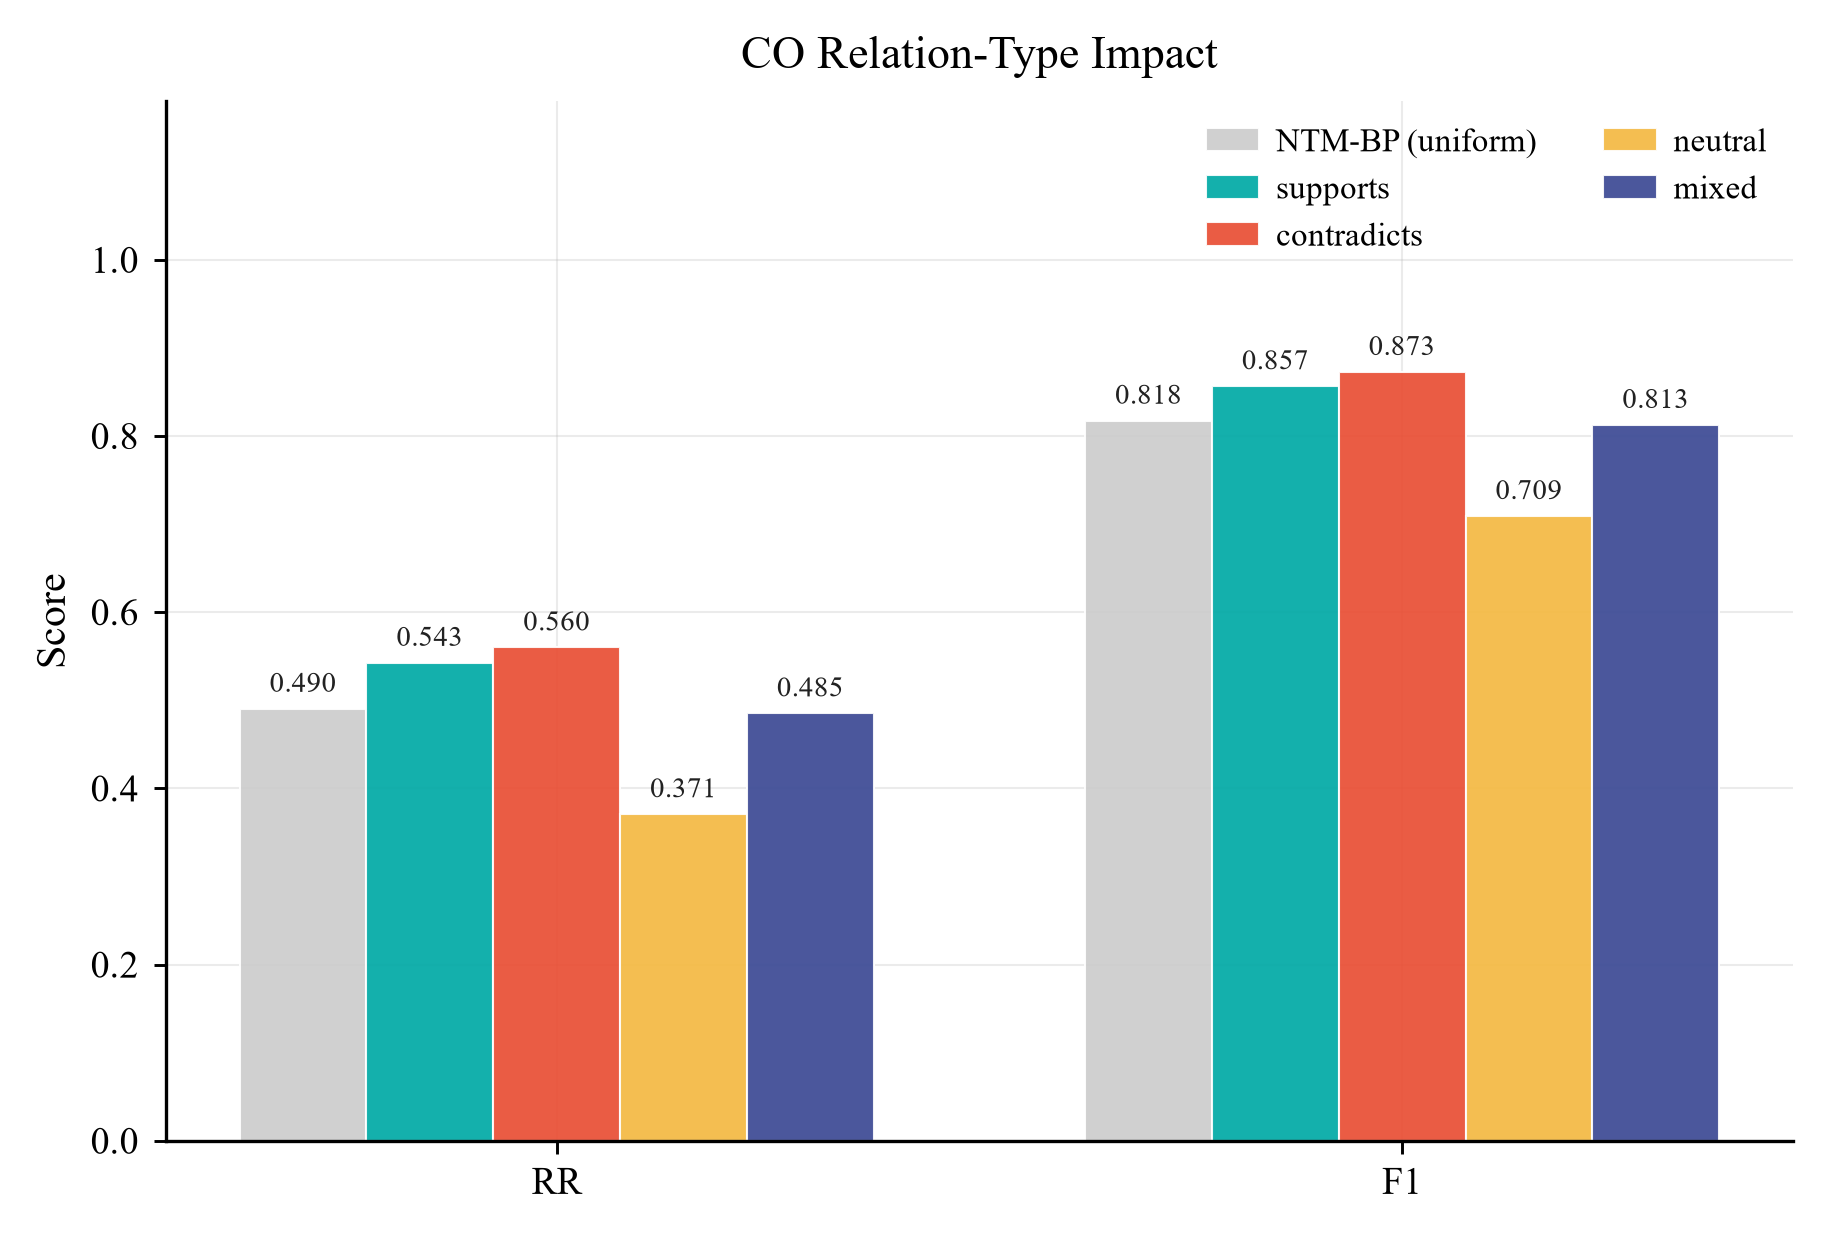
\includegraphics[width=0.92\linewidth]{figures/fig5_relation_type_impact.png}
\caption{Relation-type impact: NTM-BP vs.\ CO variants.}
\label{fig:relation-impact}
\end{figure}

\begin{figure}[t]
\centering
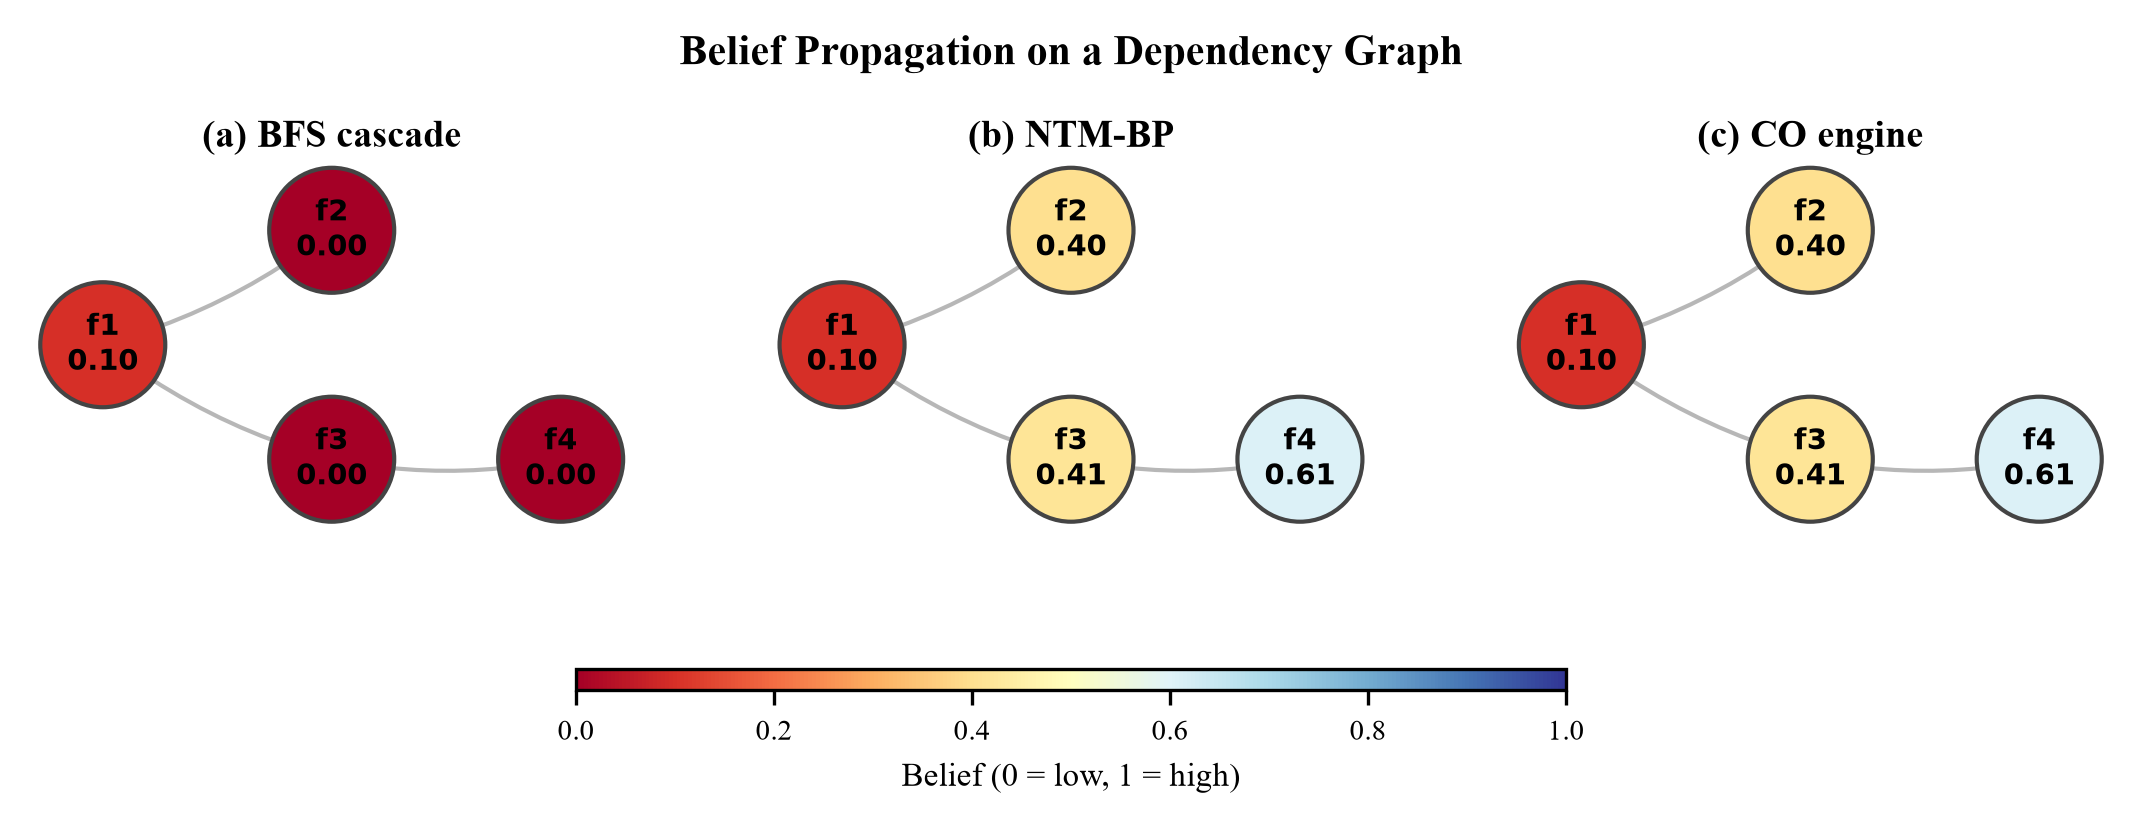
\includegraphics[width=0.96\linewidth]{figures/fig8_belief_propagation.png}
\caption{Belief propagation on a small dependency graph.  Node colors
  encode final belief values under the three engines.}
\label{fig:belief-network}
\end{figure}

\begin{figure}[t]
\centering
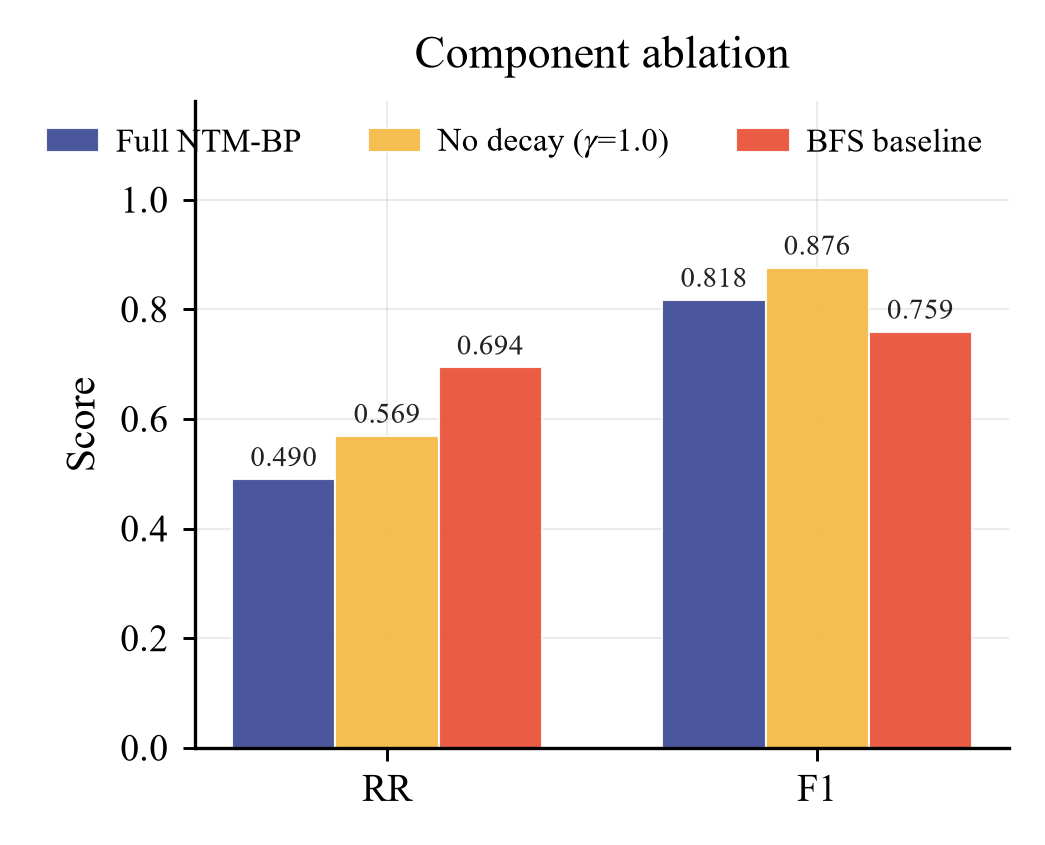
\includegraphics[width=0.78\linewidth]{figures/fig9_ablation_components.png}
\caption{Component ablation: grouped bar chart comparing Full NTM-BP,
  No-decay ($\gamma=1.0$), and BFS baseline on RR and F1.}
\label{fig:ablation-components}
\end{figure}

\begin{figure}[t]
\centering
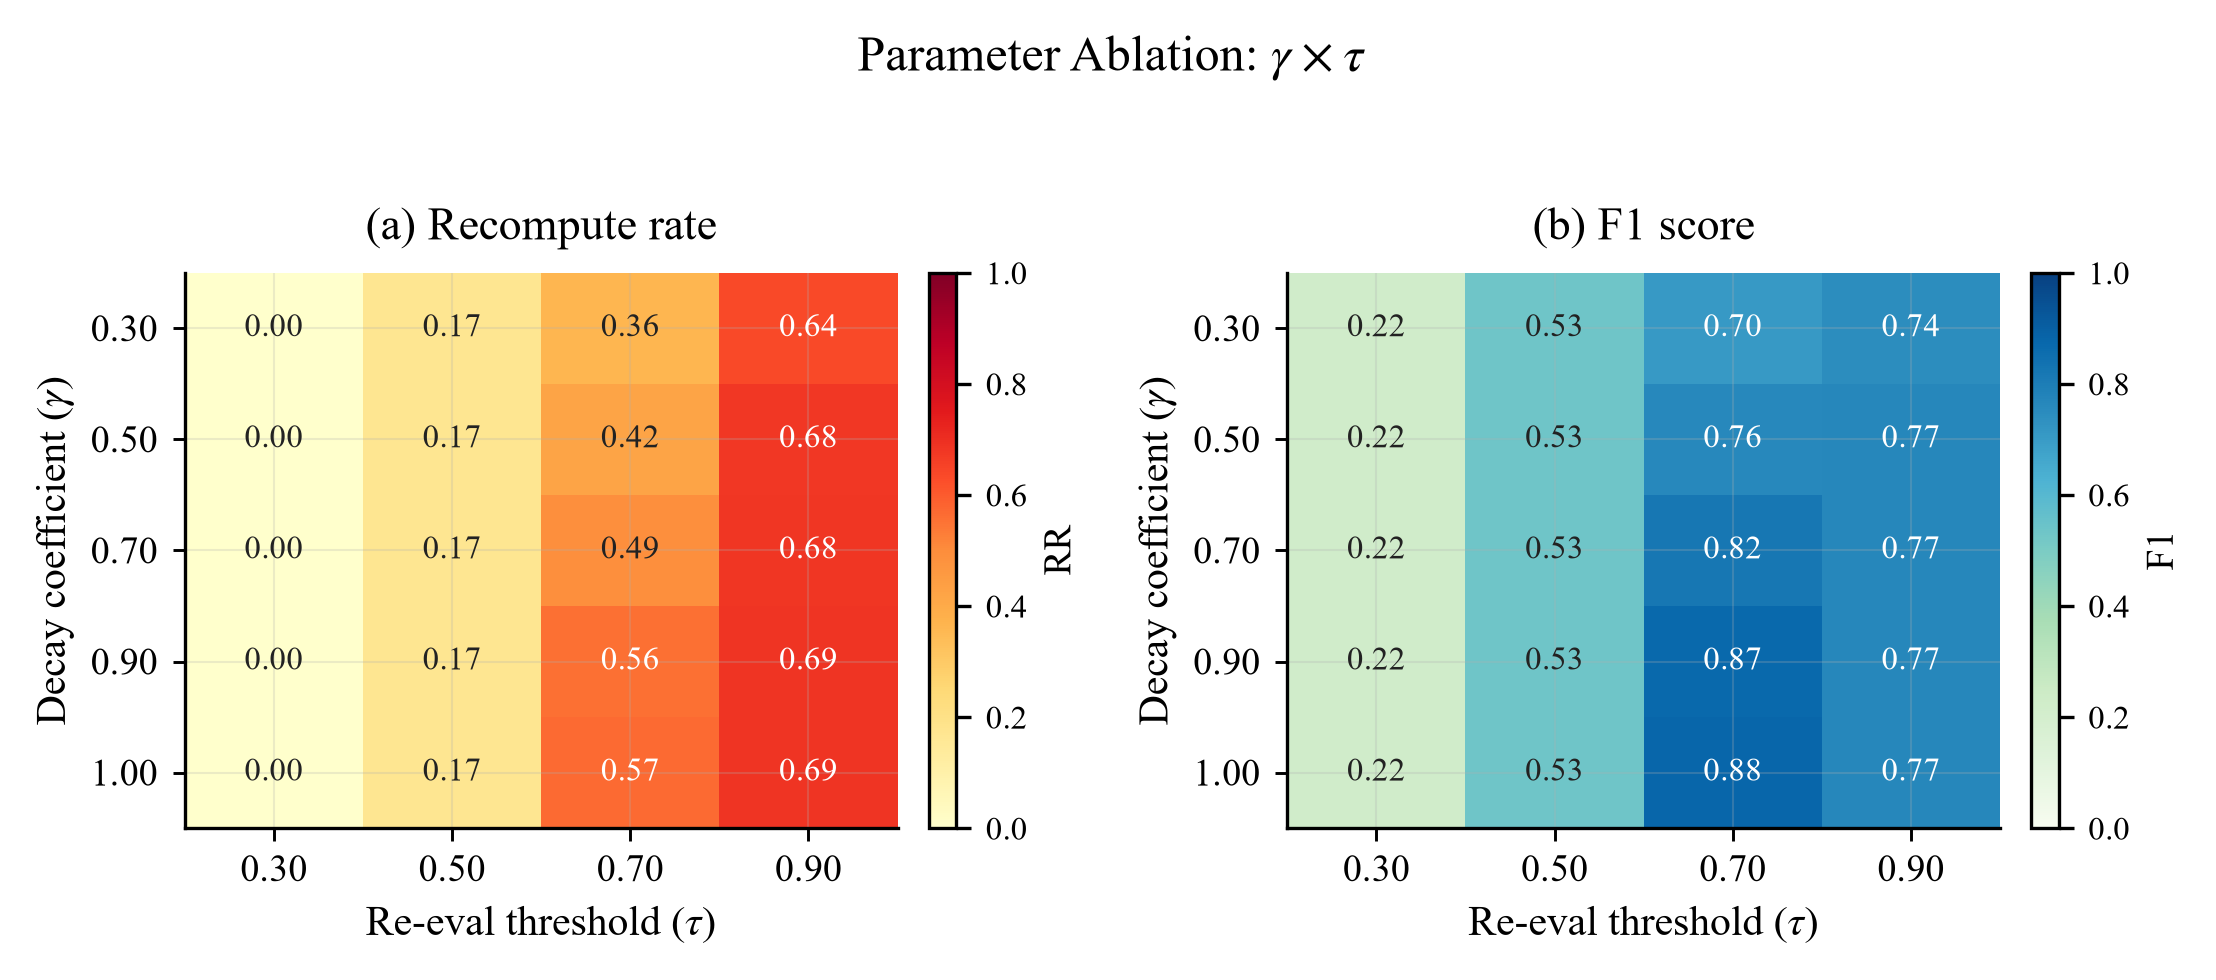
\includegraphics[width=0.95\linewidth]{figures/fig3_ablation_heatmap.png}
\caption{Two-dimensional ablation: \textbf{(a)} RR and \textbf{(b)} F1
  as functions of $(\gamma, \tau)$.}
\label{fig:heatmap}
\end{figure}

\begin{figure}[t]
\centering
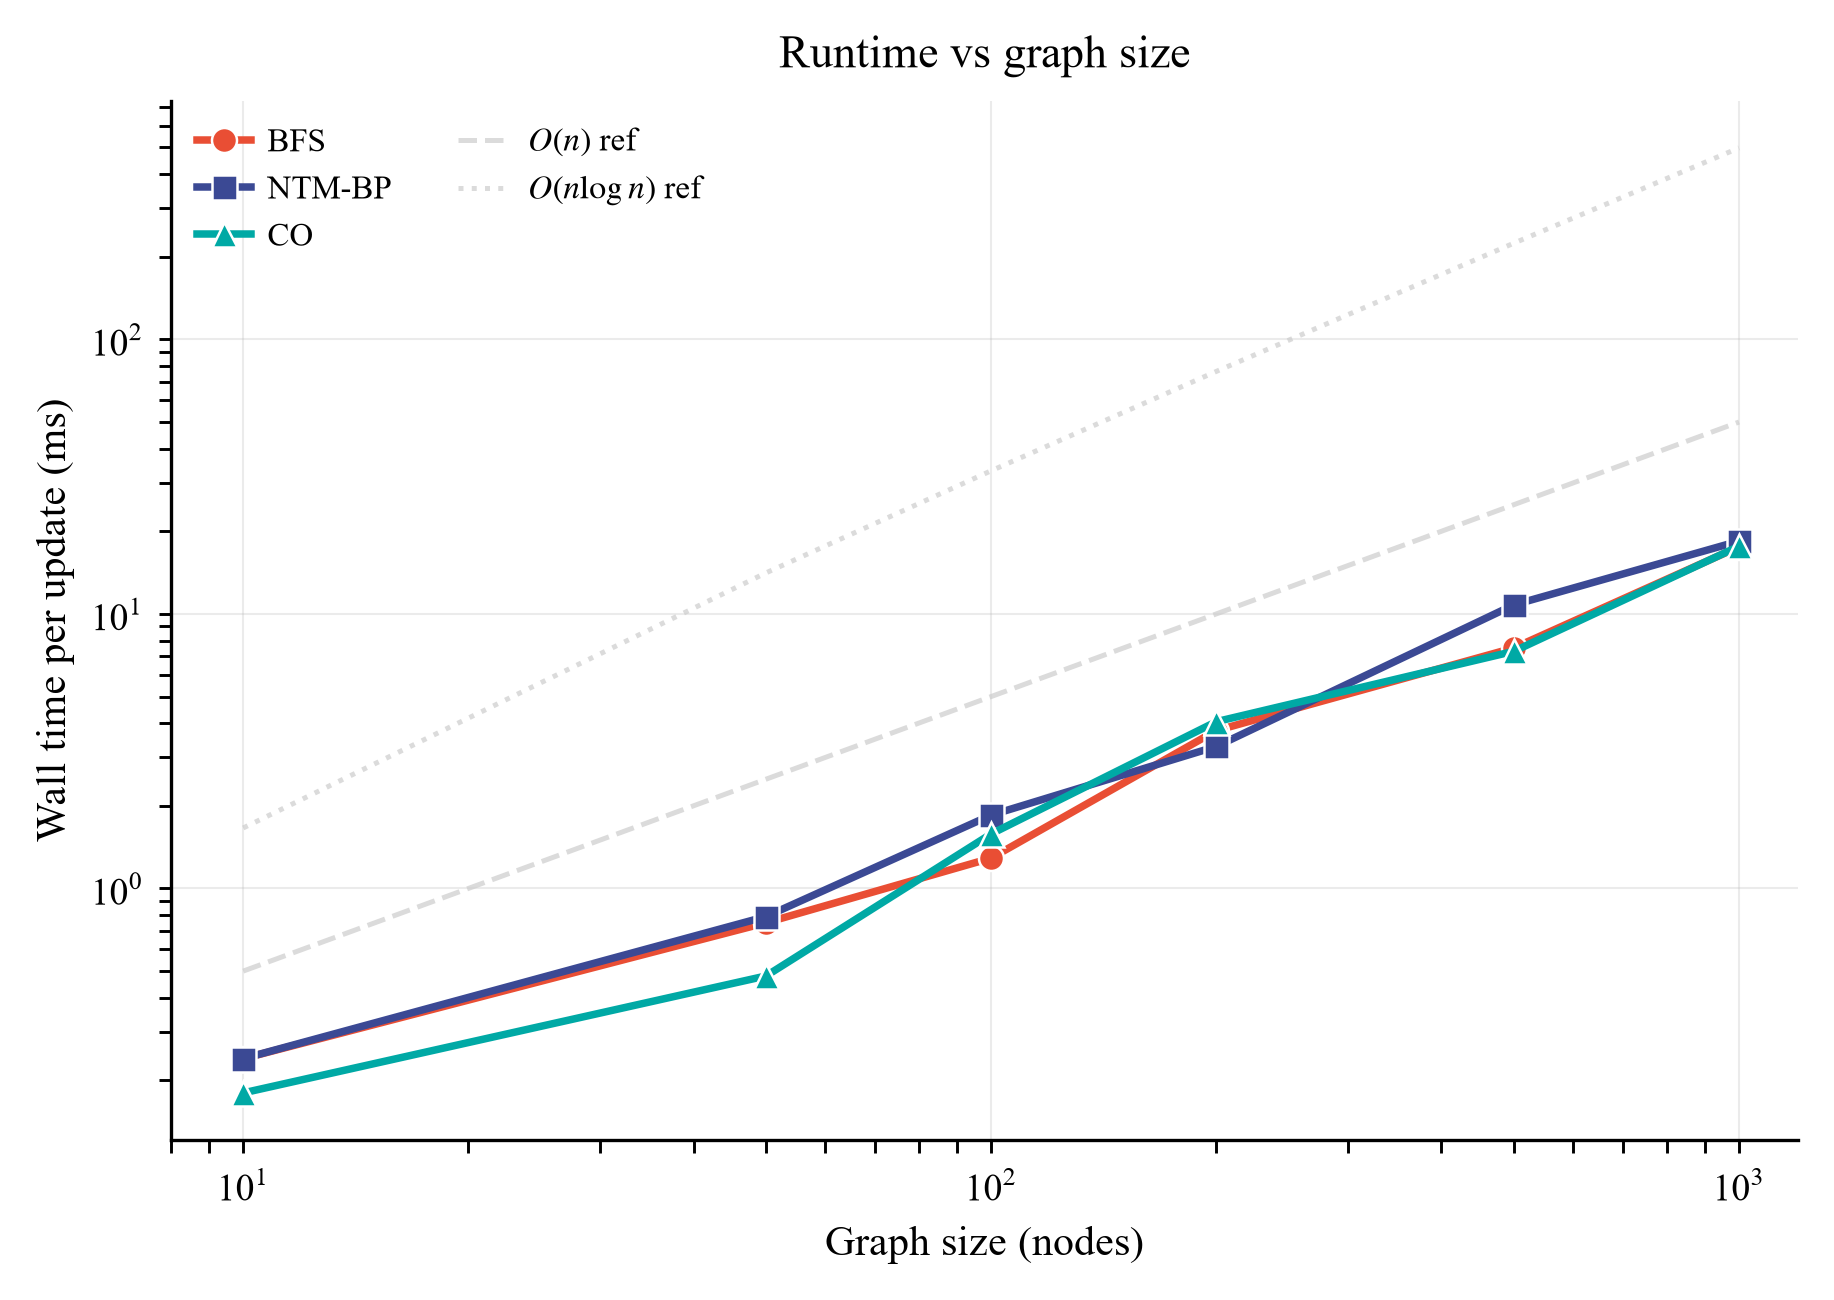
\includegraphics[width=0.92\linewidth]{figures/fig6_scalability_time.png}
\caption{Scalability: per-update wall-clock time vs.\ graph size
  (log-log).}
\label{fig:scalability}
\end{figure}

\begin{figure}[t]
\centering
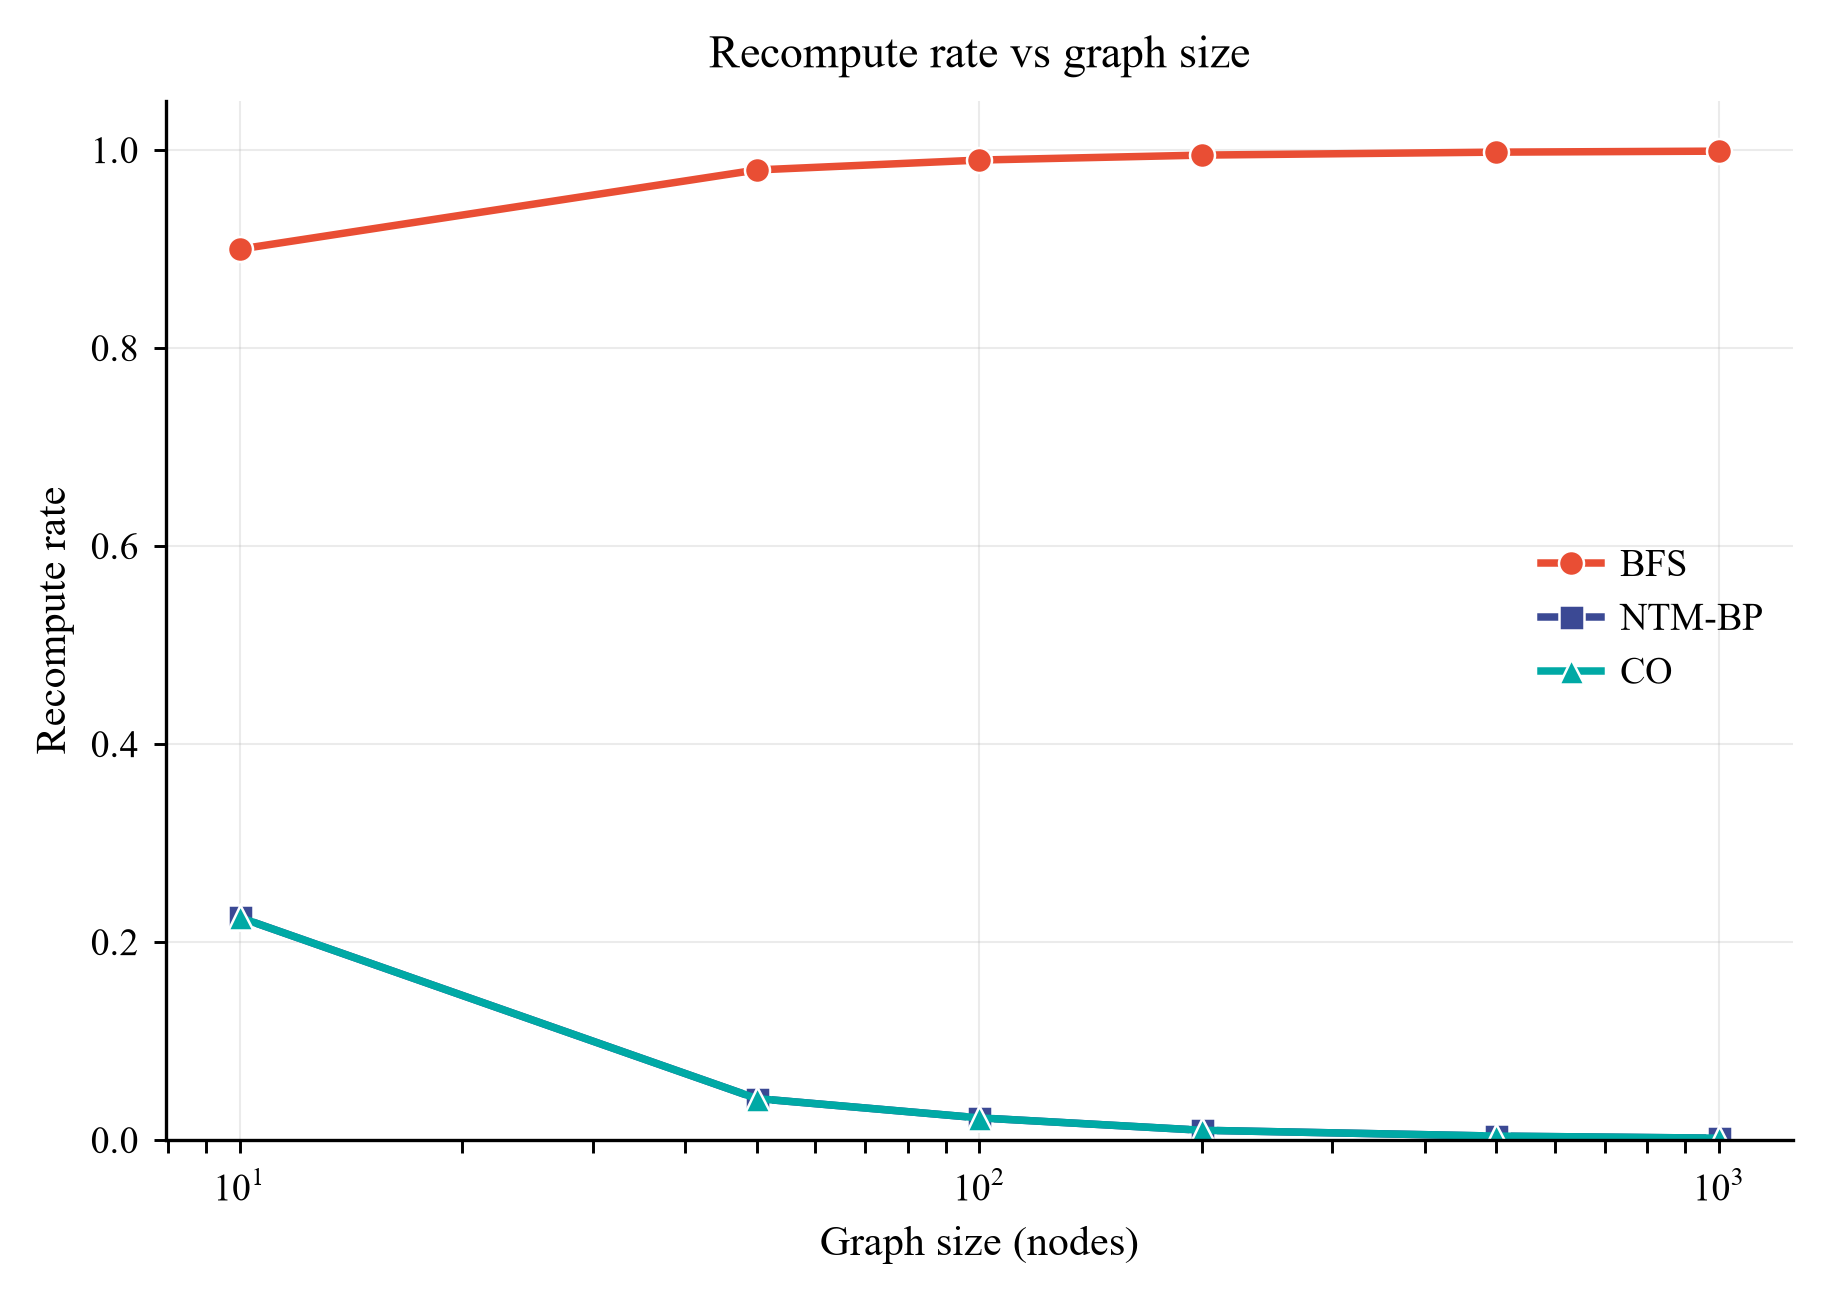
\includegraphics[width=0.80\linewidth]{figures/fig7_scalability_rr.png}
\caption{Recompute rate vs.\ graph size (semilog-$x$).}
\label{fig:scalability-rr}
\end{figure}

\textbf{Summary.}  The method fails in three diagnosable ways:
(i)~supersede-strengthening misclassification (9/54 cases, shared in
part by the scalar baseline and by the reasoning-mode probe); (ii)~a zero-cost keyword
baseline reaches F1$=0.944$ on the expansion set, bounding the
structured gate's value \emph{on that distribution} (the keyword rule
also dominates the ``unmarked'' subset, which is $31/32$ empty);
(iii)~naive
type-based routing fails ($0.750$ vs.\ $0.778$), showing that path
selection cannot substitute for accurate classification.

% ======================================================================
\section{Discussion}
\label{sec:discussion}
% ======================================================================

\subsection{Why the Structured Gate Works}

The structured gate has operational benefits beyond the intuitive
``divide and conquer'' explanation, and---as the ablation of
\cref{sec:rq3} showed---these do not require each sub-question to add a
measurable accuracy gain.  We identify three complementary mechanisms:

\textbf{Representational decoupling.}  A scalar-prompt gate must
jointly encode three orthogonal dimensions---change magnitude (Q1),
semantic relevance (Q2), and directional stance (Q3)---in a single
output token.  This creates an information bottleneck: the LLM must
simultaneously weigh evidence along all three axes and collapse them
into one decision, which empirically leads to the whac-a-mole dynamic
observed during prompt development.  The structured
decomposition removes this bottleneck by assigning each dimension a
dedicated inference call, each of which needs only to condition on the
update and its own target dimension.  The decomposition pays off
whenever each isolated sub-question is substantially easier for the LLM
than the three-way joint decision it replaces---the regime we observe in
practice, where the scalar prompt regressed
across three revision rounds while each sub-question prompt converged
independently.  We stress that this is an \emph{empirical} condition, not
a consequence of the factorization alone: the coupled error of a single
scalar decision can in principle be smaller than the combined error of
three independent ones, and the decomposition helps only because each
isolated sub-question is in practice far easier than the joint
decision.\footnote{Writing $p_1,p_2,p_3$ for the per-sub-question error
rates and $p_{\text{joint}}$ for the scalar gate's, the decomposed error
is $1-\prod_{i=1}^{3}(1-p_i)$, which expands to $p_1+p_2+p_3$ minus
higher-order terms; the decomposition is beneficial exactly when this
quantity is $<p_{\text{joint}}$, a condition not guaranteed by the
factorization alone.}

\textbf{Early-exit efficiency.}  Q1 acts as a cheap negative filter.
In the expansion set, 18 of 54 cases ($33\%$) are classified as C
(minor fluctuation) and terminate after a single LLM call.  The
expected number of calls per update under the structured gate is:
\[
\mathbb{E}[\text{calls}] = 1 +
|D_k|\cdot P(\text{Q1}\neq\text{C}) +
|D_k|\cdot P(\text{Q1}=\text{B})\cdot P(\text{Q2}=\text{yes})
\]
where $|D_k|$ is the number of downstream conclusions of the updated
fact: Q1 always costs one call; Q2 runs once per downstream conclusion
whenever Q1 exits the C path; and Q3 (the stance check) is additionally
invoked per conclusion only when Q1$=$B and Q2 is affirmative.  For the
expansion distribution audited from the frozen prompt cache
($P(\text{Q1}=\text{C})=18/54\approx 0.33$,
$P(\text{Q1}=\text{B})=9/54\approx 0.17$, $|D_k|\approx 2.28$,
$P(\text{Q2}=\text{yes})\approx 0.99$), this yields
$\mathbb{E}[\text{calls}]\approx 2.89$, and the exact audited decomposition
is $1+82/54+19/54\approx 2.87$ calls per update (Q1 once per update, Q2 once
per relevant downstream conclusion, Q3 once per stance check), matching the
measured average of $2.87$; the small gap from the closed form is the
$|D_k|$-averaging approximation.  Relative to an exhaustive three-question
evaluation of every update ($1+2|D_k|\approx 5.6$ calls), early exit
halves the expected call budget.

\textbf{Error mode isolation.}  Each failure mode of the structured
gate traces to exactly one sub-question.  The 9 losses on
expansion are all Q1 type-A over-inclusions (7 supersede $\to$ A plus 2
other over-inclusions); the 11 Q1 early-exit wins are attributable
entirely to the coarse C filter.  This one-to-one mapping between
sub-question and failure mode is the operational justification for
the decomposition: it transforms the gate-tuning problem from
``modify a scalar prompt to fix case X without breaking case Y'' into
``modify sub-question Q$_i$'s prompt to fix class-$i$ errors.''  Our
development experience provides negative evidence for this claim: every attempt
to fix a specific failure mode in the scalar prompt (v1$\to$v2$\to$v3)
introduced regression in an orthogonal failure class, while the
structured decomposition's three substantive changes
(Q1: intensify$\to$B, Q2: counterfactual, Q3: content-only) each
targeted one error class without observable cross-talk.  This mapping is
a tuning and auditing property; it does not imply that each sub-question
contributes a measurable accuracy gain---the ablation of \cref{sec:rq3}
shows Q2 and Q3 are partially redundant on the tested distribution.

\subsection{Design Principles for NTM Gates}

The empirical and theoretical results suggest five principles for
designing NTM-compatible update gates:

\begin{enumerate}
\item \textbf{Decompose when dimensions are conditionally separable.}
  If the gating decision has $k$ orthogonal semantic dimensions, and
  each dimension can be evaluated independently given the update and
  higher-priority sub-decisions, then a $k$-question decomposition
  reduces both error coupling and average cost.  The decomposition is
  beneficial precisely when the sub-questions are easier to answer
  individually than jointly---a condition that holds whenever the LLM
  exhibits the whac-a-mole pathology on the scalar version.

\item \textbf{Early-exit on the cheapest negative filter.}  Place the
  coarsest, cheapest-to-answer dimension first.  Q1 requires only the
  old and new values (no downstream context), costs one LLM call, and
  eliminates a third of updates on the expansion set.  Any gate
  design should identify a low-cost triage question that can
  immediately dismiss a non-trivial fraction of updates.

\item \textbf{Maintain a zero-cost numeric path.}  NTM-BP's F1 of
  $0.818$ on PC-500 (with decay) provides a deployment-safe fallback:
  when LLM calls are unavailable or too expensive, the numeric engine
  alone offers substantially better filtering than BFS (RR reduction
  from $0.694$ to $0.491$).  The cost-precision frontier
  (\cref{fig:pareto,tab:routing}) shows that even a simple hybrid---
  C$\to$skip, A$\to$LLM, B$\to$NTM-BP---reduces average calls below
  the structured gate, though at a precision cost.

\item \textbf{Calibrate numeric parameters on held-out data.}  The
  propagation decay $\gamma$ and saturation constant $\alpha_0$ exhibit
  smooth, monotonic control over the F1-RR tradeoff (\cref{tab:gamma}),
  but their optimal values depend on the graph topology and CPT
  distribution.  The gamma sensitivity analysis
  (\cref{sec:rq2}) provides a template: sweep $\gamma$ on a
  held-out calibration set, select the value at the elbow of the
  F1-RR curve, and report paired bootstrap confidence intervals for
  the chosen operating point.

\item \textbf{Make relation-type multipliers asymmetric, with a floor.}
  The CO engine (\cref{sec:rq4}) shows that edge-level semantic typing
  modulates propagation quality \emph{asymmetrically}: amplifying
  \texttt{supports} ($\times1.2$) and \texttt{contradicts} ($\times1.3$)
  yields F1 gains of $+3.9$ and $+5.5$, whereas dampening \texttt{neutral}
  ($\times0.5$) over-suppresses propagation and misses genuine
  re-evaluations (FNR $0.275$ vs.\ $0.108$ for uniform NTM-BP).  Since
  amplification helps more than dampening hurts, relation-type multipliers
  $m_r$ should be floored to prevent excessive suppression---e.g.,
  $\max(0.5,\min(1.5,m_r))$, so no edge type drops propagation below half
  the uniform baseline.  Learning these multipliers (via a small
  calibrated classifier rather than fixed constants) and integrating CO's
  edge-type signal with the gate's Q3 stance judgment are natural
  extensions.
\end{enumerate}

\subsection{Limitations and Future Work}
\label{sec:limitations}

\textbf{Supersede-strengthening misclassification.}  The primary
failure mode---Q1 reading supersede-style strengthening (``all-time
high,'' ``perfect score'') as a directional change (A), 9 of 54
expansion cases---is characterized in full in \cref{sec:rq4}, together
with the evidence that it is a tendency of this model and prompt pair
rather than a decomposition artifact: the frozen scalar gate (gate-v1)
fails on 7 of the 9 cases, and the reasoning mode of the same model
(\texttt{deepseek-reasoner}) corrects 6 of the 10 supersede cases but
not all; we do not repeat that analysis here.  (The
scalar prompt received two tracked refinement rounds
(v1$\to$v2$\to$v3), but its improvements saturated early---the asymmetry
reflects diminishing returns on the coupled scalar path, not unequal
effort.)  Three fix strategies are available, ordered
by invasiveness: (a) refine Q1's definition to explicitly enumerate
``state-surpassed-but-direction-unchanged'' as class B (zero
architectural change, but requires new held-out data for ex-ante
validation); (b) add a Q1.5 sub-question that discriminates
supersession from true directional change only when Q1 returns A (adds
one conditional LLM call on $\sim 40\%$ of updates); (c) replace the
discrete A/B/C classification with a continuous change-magnitude score
and threshold it jointly with a semantic direction detector (requires
architectural redesign).  Strategy (a) is the natural next step,
pending a fresh held-out dataset to preserve the one-shot evaluation
discipline.

\textbf{LLM dependency and cost.}  The structured gate requires LLM
calls (audited average $2.87$ per update on expansion, corresponding to
$\sim 850$ input tokens and $\sim 120$ output tokens per call
under DeepSeek-V4-Flash, or approximately $\$0.0010$~USD per update at
the provider's published pricing at the time of the experiments
($2.87$ calls $\times$ ($850$ input $+$ $120$ output tokens); unit prices
are provider- and date-specific),
making it unsuitable for latency-critical
paths.  Both the per-call token counts and the $\$0.0010$ figure are
specific to this provider and its published pricing at the time this
work was run; they will shift with any change of model, tokenizer, or
price schedule, so the cost numbers should be read as an
order-of-magnitude illustration rather than a durable constant.  The decomposition is not free even relative to scalar gating:
the structured gate costs about $26\%$ more calls per update than
gate-v1 ($2.87$ vs.\ $2.28$) on the expansion set, and its
point-estimate F1 advantage over gate-v1 is not statistically significant
(\cref{tab:expansion}); a single-call gate that answers all three
dimensions jointly would be the natural cost-matched baseline, and
building one is future work.  However, the cost structure is
distribution-dependent: the
expected cost scales with $1-P(\text{Q1}=\text{C})$, so domains with
many minor fluctuations benefit disproportionately from the early-exit
path.  In the worst case (all updates are type-B with every downstream
conclusion relevant), the structured gate costs $1+2|D_k|$ calls per
update (Q1, one Q2 per conclusion, one Q3 per conclusion)---still
bounded by the update's downstream closure, but roughly twice the
naive per-conclusion evaluation; the benefit in this regime is
error-mode isolation rather than call savings.
The zero-cost NTM-BP fallback (F1$ =0.818$,
RR$ =0.491$ on PC-500) provides a practical alternative: systems can
deploy NTM-BP only and accept the $9$-point F1 gap on the expansion
set ($0.686$ vs.\ $0.778$; the two are statistically tied at $0.85$ on
PC-500), or run the
structured gate on a sampled subset of updates for quality assurance
while relying on NTM-BP for the remainder.

\textbf{Lexical boundary condition.}  The zero-cost keyword baseline
of \cref{tab:kwbaseline} outperforms the structured gate on
Expansion-500 (F1 $0.944$ vs.\ $0.778$; paired $\Delta=+0.167$,
$p<0.001$).  This is a genuine, distribution-specific boundary of our
claim: when impact-bearing updates carry overt lexical cues and the
confidence delta is available, a rule needs no semantic inference, and on
that distribution we do not claim a gate advantage.  The structured
gate's value claim is therefore scoped to (i) updates whose impact is
\emph{not} lexically marked---on the balanced adversarial set of
\cref{sec:balanced} the gate is significantly better than the rule
($p=0.001$)---and (ii) auditability: each gate decision decomposes into
logged sub-answers that a deployed system can inspect.  (On the
Expansion-500 ``unmarked'' subset itself a conservative rule also scores
well, because $31$ of those $32$ cases are empty; we do not read that
subset as evidence of semantic skill.)  Quantifying the prevalence of
lexically unmarked updates in real
agent traffic is the key open question that decides how much of the
frontier belongs to rules versus LLM gates.

\textbf{Dependency graph extraction.}  Our experiments assume the
dependency graph $G$ is given.  Real deployment must extract
\texttt{depends\_on} edges from unstructured agent dialogue.  This
introduces two error types: missing edges (false negatives in the
graph, causing missed re-evaluations downstream) and spurious edges
(false positives, causing unnecessary propagation).  Missing edges
are the more dangerous failure mode because they break the dependency
completeness axiom and can leave genuinely invalidated conclusions
unflagged.  Spurious edges degrade precision but preserve recall---the
safer failure direction for high-stakes applications, where missed
invalidation is costlier than unnecessary re-computation.  A pragmatic
intermediate is to extract edges via structured CoT prompting (where
the LLM explicitly cites source facts in its reasoning chain), which
yields high-precision edges at the cost of constraining the LLM's
output format.  Graph extraction quality is orthogonal to the gating
problem but determines the upper bound on any downstream gate's recall;
we therefore recommend a high-recall, modest-precision extraction
strategy.  A pilot experiment on CoT-extracted
edges (with manual verification as ground truth) is planned as
immediate future work to quantify the extraction-to-propagation error
cascade.

\textbf{Non-tree graphs.}  \cref{thm:convergence} guarantees
convergence only for acyclic graphs.  Real dependency graphs may
contain cycles (e.g., mutual reinforcement between ``delivery risk
is manageable'' and ``supplier reliability is adequate'').  The
implemented Algorithm~\ref{alg:ntmbp} maintains a \emph{visited} set,
so each node is processed at most once and the algorithm terminates
after a single forward pass on any finite graph; on a cyclic graph this
pass is well-defined but is not guaranteed to reach a fixed point.
More subtly, on a \emph{multi-parent} DAG---acyclic but not a tree, with
several incoming paths to the same node---processing each node once means
only the first-arriving path contributes to its belief, so the result can
depend on traversal order and need not equal a proper aggregation over all
paths.  The convergence guarantee and calibration above are therefore stated
for trees (unique root-to-node paths), and correct multi-path aggregation
remains future work.
Remark~\ref{rem:loopy} analyzes the linearized fixed-point model of the decay
update as a theoretical extension of NTM-BP to loopy graphs; extending
the implemented multiplicative rule to iterate toward that fixed point,
and a formal proof, remain future work.

% Sec. 6.4 (NTM-BP internal properties and the CO engine) was folded
% into the design principles above: its genuinely new content (the
% asymmetric relation-type multiplier with a floor) is now principle 5 in
% \cref{sec:discussion}, and the saturating/gamma/scalability restatements
% were removed as duplicative of Tables 4--7 and the Conclusion.

% ======================================================================
\section{Conclusion}
% ======================================================================

We presented a selective belief propagation framework for truth maintenance
in LLM agent memory, replacing binary STALE marking with continuous belief
propagation.  Two complementary mechanisms---numeric NTM-BP and the
structured semantic gate---offer different points on the
cost-precision frontier.  The structured gate, with its three-way
decomposition into change type, relevance, and stance, achieves the
highest point estimate among the evaluated non-lexical methods on a
fully held-out validation set (54 never-seen
cases, dual-annotator labels, $\kappa=1.0$), with its strongest
statistically supported advantage being over the BFS baseline ($+0.463$,
$p<0.001$).  On that distribution a zero-cost keyword rule matches or
beats the gate, so we do not claim a gate advantage there; on a second,
balanced adversarial held-out set whose impact signal is deliberately
\emph{not} lexically marked, the structured gate is significantly more
accurate than both NTM-BP ($+0.110$, $p<0.001$) and the keyword rule
($+0.250$, $p=0.001$), locating the decomposition's value to the
regime where surface cues are absent.  Its gains come primarily from
correctly skipping minor
fluctuations (the 11 type-C wins, among 18 type-C cases resolved with a
single LLM call), while its losses are concentrated in a single,
diagnosable failure mode---an over-inclusive class-A boundary that
misreads supersede-strengthening updates as directional changes---shared
in part by the scalar-prompt baseline and by the reasoning-mode probe.

Internal validation reveals that NTM-BP is more than a baseline:
the saturating source-change scaling eliminates the ``identical cascade
for any update'' pathology; the propagation decay $\gamma$ yields a
smooth F1-RR tradeoff, with paired differences from the no-decay baseline
significant for $\gamma\le0.8$
($\gamma=0.7$: F1$ =0.818$, RR$ =0.491$ vs.\ BFS RR$ =0.694$); and
the engine scales linearly with graph size ($<20$~ms on
$1{,}000$ nodes).  The CO engine further demonstrates that
edge-level semantic typing can improve propagation quality (up to
$+5.5$ F1 on contradicts chains), though with a cautionary tradeoff
on neutral chains.  A naive type-based routing strategy fails
($0.750$ vs.\ $0.778$), demonstrating that path selection cannot
substitute for accurate classification.  Future work on Q1
refinement, automatic dependency-graph extraction, and robust
relation-type annotation can further close the remaining gap.

% ======================================================================
% AUTHOR CONTRIBUTIONS
% ======================================================================

\section*{Author Contributions}

\textbf{Yuhan Feng} --- Conceived the research problem from personal
experience with LLM coding agents and a biology-inspired analogy of
graded (rather than binary) responses; designed the NTM-BP algorithm
(continuous belief propagation replacing binary STALE flags) and the
Structured Semantic Gate (three-way Q1/Q2/Q3 decomposition). Directed and
audited the full Python implementation---specified the architecture,
dataset design, and evaluation goals, and audited all code logic,
formulas, and results; the code and experiment scripts were developed
under the author's direction, with AI providing syntax- and
debugging-level assistance. Designed
and conducted all experiments,
including the main benchmarks (PC-500, SynDep, Expansion-500,
CO-Relation), the ablations over $\gamma$, CPT and walk-sum conditions,
the keyword baselines, and the routing simulation. Performed iterative
optimization, debugging, and manuscript writing, and prepared all
supplementary materials.

% ======================================================================
% REFERENCES
% ======================================================================

\clearpage
{\small
\begin{thebibliography}{99}

\bibitem{malioutov2006walksum}
D.~M.~Malioutov, J.~K.~Johnson, and A.~S.~Willsky.
\newblock Walk-sums and belief propagation in {Gaussian} graphical
  models.
\newblock {\em Journal of Machine Learning Research}, 7:2031--2064,
  2006.

\bibitem{doyle1979tms}
J.~Doyle.
\newblock A truth maintenance system.
\newblock {\em Artificial Intelligence}, 12(3):231--272, 1979.

\bibitem{dekleer1986atms}
J.~de~Kleer.
\newblock An assumption-based {TMS}.
\newblock {\em Artificial Intelligence}, 28(2):127--162, 1986.

\bibitem{agm1985}
C.~E. Alchourr\'{o}n, P.~G\"{a}rdenfors, and D.~Makinson.
\newblock On the logic of theory change: Partial meet contraction and
  revision functions.
\newblock {\em Journal of Symbolic Logic}, 50(2):510--530, 1985.

\bibitem{pearl1988}
J.~Pearl.
\newblock {\em Probabilistic Reasoning in Intelligent Systems: Networks of
  Plausible Inference}.
\newblock Morgan Kaufmann, 1988.

\bibitem{memgpt}
C.~Packer, S.~Wooders, K.~Lin, V.~Fang, S.~G.~Patil, I.~Stoica, and
  J.~E.~Gonzalez.
\newblock {MemGPT}: Towards {LLMs} as operating systems.
\newblock {\em arXiv:2310.08560}, 2023.

\bibitem{mem0}
P.~Chhikara, D.~Khant, S.~Aryan, T.~Singh, and D.~Yadav.
\newblock {Mem0}: Building production-ready {AI} agents with scalable
  long-term memory.
\newblock {\em arXiv:2504.19413}, 2025.

\bibitem{letta}
Letta AI.
\newblock {Letta}: The memory-first agent framework.
\newblock Software documentation, \url{https://letta.com}, 2026.
  Accessed August 2026.

\bibitem{zep}
P.~Rasmussen, P.~Paliychuk, T.~Beauvais, J.~Ryan, and D.~Chalef.
\newblock {Zep}: A temporal knowledge graph architecture for agent
  memory.
\newblock {\em arXiv:2501.13956}, 2025.

\bibitem{kumiho2026}
Y.~B. Park.
\newblock Graph-native cognitive memory for {AI} agents: Formal belief
  revision semantics for versioned memory architectures.
\newblock {\em arXiv:2603.17244}, 2026.

\bibitem{retroformer2023}
W.~Yao, S.~Heinecke, J.~C.~Niebles, Z.~Liu, Y.~Feng, L.~Xue,
  R.~Murthy, Z.~Chen, J.~Zhang, D.~Arpit, R.~Xu, P.~Mui, H.~Wang,
  C.~Xiong, and S.~Savarese.
\newblock {Retroformer}: Retrospective large language agents with
  policy gradient optimization.
\newblock In {\em ICLR}, 2024.

\bibitem{sclar2024prompt}
M.~Sclar, Y.~Choi, Y.~Tsvetkov, and A.~Suhr.
\newblock Quantifying language models' sensitivity to spurious features in
  prompt design, or: How I learned to start worrying about prompt
  formatting.
\newblock In {\em ICLR}, 2024. (arXiv:2310.11324.)

\bibitem{magma2026}
D.~Jiang, Y.~Li, G.~Li, and B.~Li.
\newblock {MAGMA}: A multi-graph based agentic memory architecture for
  {AI} agents.
\newblock In {\em Proceedings of the 64th Annual Meeting of the
  Association for Computational Linguistics (ACL)}, 2026, to appear.
  (arXiv:2601.03236.)

\bibitem{amem2026}
W.~Xu, Z.~Liang, K.~Mei, H.~Gao, J.~Tan, and Y.~Zhang.
\newblock {A-MEM}: Agentic memory for {LLM} agents.
\newblock In {\em NeurIPS}, 2025.

\bibitem{longmemeval}
D.~Wu, H.~Wang, W.~Yu, Y.~Zhang, K.-W.~Chang, and D.~Yu.
\newblock {LongMemEval}: Benchmarking chat assistants on long-term
  interactive memory.
\newblock In {\em ICLR}, 2025.

\bibitem{react2023}
S.~Yao, J.~Zhao, D.~Yu, N.~Du, I.~Shafran, K.~Narasimhan, and Y.~Cao.
\newblock {ReAct}: Synergizing reasoning and acting in language models.
\newblock In {\em ICLR}, 2023.

\bibitem{koller2009probabilistic}
D.~Koller and N.~Friedman.
\newblock {\em Probabilistic Graphical Models: Principles and Techniques}.
\newblock MIT Press, 2009.

\bibitem{rag2020}
P.~Lewis, E.~Perez, A.~Piktus, et~al.
\newblock Retrieval-augmented generation for knowledge-intensive {NLP}
  tasks.
\newblock In {\em NeurIPS}, 2020.

\bibitem{hansson1999revision}
S.~O.~Hansson, A.~Ferm\'e, J.~Cantwell, and M.~Falappa.
\newblock Credibility limited revision.
\newblock {\em Journal of Symbolic Logic}, 66(4):1581--1596, 2001.

\bibitem{park2023generative}
J.~Park, J.~C.~O'Brien, C.~J.~Cai, M.~R.~Morris, P.~Liang, and
  M.~S.~Bernstein.
\newblock Generative agents: Interactive simulacra of human behavior.
\newblock In {\em UIST}, 2023.

\bibitem{yushuai2025memorybench}
Q.~Ai, Y.~Tang, C.~Wang, J.~Long, W.~Su, and Y.~Liu.
\newblock Memory{B}ench: A benchmark for memory and continual learning
  in {LLM} systems.
\newblock {\em arXiv:2510.17281}, 2025.

\bibitem{stale2026}
H.~Chao, Y.~Bai, R.~Sheng, T.~Li, and Y.~Sun.
\newblock {STALE}: Can {LLM} agents know when their memories are no longer
  valid?
\newblock {\em arXiv:2605.06527}, 2026.

\bibitem{memtx2026}
X.~Li et~al.
\newblock {MemTX}: Transactional belief commit for stateful agent memory.
\newblock {\em arXiv:2607.23929}, 2026.

\bibitem{meme2026}
S.~Jung, A.~Rubinstein, A.~Uselis, S.~Yun, and S.~J.~Oh.
\newblock {MEME}: Multi-entity \& evolving memory evaluation.
\newblock {\em arXiv:2605.12477}, 2026.

\bibitem{supersede2026}
V.~Patel.
\newblock {Supersede}: Diagnosing and training the memory-update gap in
  {LLM} agents.
\newblock {\em arXiv:2606.27472}, 2026.

\bibitem{past2026}
Z.~Chen, S.~Dong, C.~Shi, P.~Wang, S.~Wang, C.~Shen, and J.~Li.
\newblock The past is prologue: A plug-in controller for selective
  updates in sequentially evolving {LLM} memory.
\newblock {\em arXiv:2606.31121}, 2026.

\bibitem{thom2020justifications}
T.~Fr\"uhwirth.
\newblock Justifications in constraint handling rules for logical
  retraction in dynamic algorithms: Theory, implementations, and
  complexity.
\newblock {\em Fundamenta Informaticae}, 173(4):253--283, 2020.

\bibitem{fazio2021logicalgebraic}
D.~Fazio and M.~Pra Baldi.
\newblock On a logico-algebraic approach to {AGM} belief contraction
  theory.
\newblock {\em Journal of Philosophical Logic}, 50(5):911--938, 2021.

\bibitem{massimiliano2022paraconsistent}
M.~Carrara, D.~Fazio, and M.~Pra Baldi.
\newblock Paraconsistent belief revision: An algebraic investigation.
\newblock {\em Erkenntnis}, 89(2):725--753, 2022.

\bibitem{han2026temporal}
G.~Han, W.~Chen, X.~Zhang, L.~Zhang, A.~Liu, and L.~Zhao.
\newblock When temporal knowledge graph meets multi-modality: A new
  perspective for temporal knowledge graph forecasting.
\newblock {\em Information Processing and Management},
  63(2):104463, 2026.

\bibitem{rui2015causal}
R.~Chang, J.~R. Karr, and E.~E. Schadt.
\newblock Causal inference in biology networks with integrated belief
  propagation.
\newblock {\em Pacific Symposium on Biocomputing}, pages 359--370, 2015.

\bibitem{sun2025senticnet}
X.~Sun, J.~Qi, Z.~Zhu, M.~Li, H.~Pei, and J.~Meng.
\newblock {SenticNet} and abstract meaning representation driven
  attention-gate semantic framework for aspect sentiment triplet
  extraction.
\newblock {\em Engineering Applications of Artificial Intelligence},
  139:109625, 2025.

\end{thebibliography}
}

% ======================================================================
% ACKNOWLEDGMENTS (standalone page, placed after the references)
% ======================================================================

\clearpage
\section*{Acknowledgments}

\noindent\textbf{Research origin and background.}
This work grew out of the author's hands-on experience using LLM coding
agents on personal projects, rather than from formal training in agent
research. The author found the STALE work~\cite{stale2026}---whose CUPMem
propagates discrete KEEP/STALE/REPLACE states---particularly interesting,
and applied its idea in an LLM agent built by the author. In doing so, the
author observed that whenever a stored fact was updated, existing
downstream conclusions were simply flagged invalid and recomputed in an
uncontrolled cascade, inflating inference cost and failing to distinguish
minor fluctuations from genuine reversals. Drawing an analogy from
biology---where states and responses are typically graded rather than
binary---the author proposed the core idea of replacing that binary
stale/valid judgment with a continuous $0$--$1$ belief value propagated
over a dependency graph. The author then validated the direction's basic
feasibility and wrote a first draft of the paper and its formal proofs
himself, before refining the exposition with AI assistance and the
advisors' guidance.

\noindent\textbf{Advisors.}
The advisors for this research are Mr.~Shu Shi and Mr.~Li Zixuan, both
teachers at Zhuzhou Nanfang High School. Both are the author's teachers
and stand in an advisor--student relationship with the author; neither is
a co-author. Mr.~Shu Shi provided the computing hardware and runtime
environment used in this study, and assisted with technical documentation
and writing feedback. During the research implementation stage, he
continuously monitored the project's progress, reminded the author of
milestone tasks so that the work stayed on schedule and was not abandoned
midway, promptly helped the author identify and resolve difficulties
encountered, and corrected non-standard practices to ensure that the
research process remained scientifically rigorous. Mr.~Li Zixuan provided
ongoing mentorship and manuscript-writing guidance throughout the project,
and assisted the author with paper revision, plagiarism checking, and
workflow organization. The advising by both teachers was \textbf{unpaid};
the author provided no compensation, direct or indirect, to either
advisor, and this research received no guidance or funding from any
training or for-profit institution. Neither advisor is a co-author; their
role was limited to the support described above, and the core intellectual
contributions remain the author's own.

\noindent\textbf{Division of work across the research process.}
The author directed the research; the breakdown is as follows:
\begin{itemize}
  \item \textbf{Topic selection and problem formulation}: independently
    proposed by the author from personal experience with LLM agents, with
    idea-level discussion with the two advisors and AI.
  \item \textbf{Theoretical modeling and proofs}: the author formalized
    the continuous belief state, the probabilistic dependency graph, and
    the binary-to-continuous generalization of Doyle's
    TMS~\cite{doyle1979tms}, and independently wrote the first draft of
    the theorems and proofs; AI assisted with wording polishing and
    derivation checking.
  \item \textbf{Algorithm design}: the author proposed the overall NTM-BP
    design (multiplicative belief decay, saturating source-change scaling,
    propagation decay coefficient $\gamma$, and priority-queue message
    passing) and the three-question decomposition of the Structured
    Semantic Gate; AI offered suggestions at the idea-optimization level,
    and the author determined and verified the final design.
  \item \textbf{Code implementation and debugging}: the author set the
    program structure and evaluation goals; the codebase and experiment
    scripts were developed under the author's direction, with AI
    assisting at the syntax- and debugging level; the author audited all
    code logic, formulas, and results item by item.
  \item \textbf{Data acquisition and annotation}: the author designed the
    dataset templates and served as the first annotator; Mr.~Li Zixuan
    independently completed a blinded annotation without access to
    existing labels or engine outputs, with perfect agreement
    ($\kappa = 1.0$). Because the second annotator is also the author's
    advisor rather than a fully disinterested third party, the perfect
    agreement is treated as a consistency check on the annotation policy
    rather than independent external validation.
  \item \textbf{Experimental design and execution}: the research
    objectives, evaluation goals, and concrete experimental protocol were
    set and checked by the author; AI assisted with data-analysis tooling
    and script debugging under the author's direction; the author
    executed the protocol, reviewed and validated the final protocol, and
    audited every reported result.
  \item \textbf{Manuscript writing, checking, and optimization}: the
    author wrote the manuscript body, all figures, tables, pseudocode, and
    appendices; AI assisted with English polishing, structural
    organization, argumentation optimization, visual and formatting
    consistency, and a final pass for typos and internal inconsistencies;
    the author reviewed and confirmed all of these, and verified the
    authenticity and citation correspondence of every reference.
\end{itemize}

\noindent\textbf{Difficulties encountered and resolution.}
\begin{itemize}
  \item \textit{Whac-a-mole coupling in the monolithic scalar-prompt
    gate}: iterative prompt tuning introduced regressions across disjoint
    failure modes; resolved by decomposing the reasoning into three
    orthogonal sub-questions Q1/Q2/Q3, enabling independent convergence.
  \item \textit{Supersede-strengthening misclassification} (``all-time
    high'' judged as a directional change); identified as a behavioural
    tendency of this model--prompt pair that the reasoning mode reduces
    but does not eliminate, documented as the primary remaining failure
    case, with three mitigation strategies (\cref{sec:limitations}).
  \item \textit{The zero-cost keyword baseline outperformed the structured
    gate} (F1 $0.944$ vs.\ $0.778$); interpreted as a lexical-signal
    boundary condition.
  \item \textit{Naive type-based routing underperformed classification}
    ($0.750$ vs.\ $0.778$); the negative finding was retained without
    post-hoc discarding.
\end{itemize}

\noindent\textbf{AI-usage declaration (per competition rules).}
\begin{itemize}
  \item \textbf{Tools and versions}: Doubao (ByteDance); OpenCode, an
    open-source coding agent, used with the assistant models available to
    the author---the provider's built-in models and the DeepSeek API; and
    the DeepSeek API chat model (identifier \texttt{deepseek-chat}; the
    provider's changelog (2026-04-24) lists this alias as corresponding
    to the non-thinking mode of DeepSeek-V4-Flash) together with
    \texttt{deepseek-reasoner} (the thinking mode of the same model).
    Exact per-session model identifiers and per-call records are recorded
    in the submitted chat logs and API records.
  \item \textbf{Stages and purposes}: Doubao for early exploratory direction
    validation and prototype discussion; OpenCode for code debugging and
    experiment-script assistance, data-analysis assistance, language
    polishing, structural organization, and literature-search leads; the
    DeepSeek API for the
    LLM semantic-gate evaluations under frozen prompts
    (temperature $0.1$); \texttt{deepseek-reasoner} as a reasoning-mode
    diagnostic probe. AI was additionally used for final manuscript
    checks (typos and internal inconsistencies), visual/format
    unification, and structure/argumentation optimization. All cited
    literature was verified for existence and citation accuracy by the
    author; AI use was approved by both advisors in advance.
  \item \textbf{Timing and frequency}: approximately 20 tracked assistant
    sessions between July and September 2026; total LLM API expenditure
    below \$5~USD.
  \item \textbf{Manual verification and boundary}: the author's own
    contributions are the identification of the problem from personal
    experience, the core idea, the overall research direction, the first
    draft of the formal proofs, the experimental design, and the reported
    analysis. AI assisted with code debugging, data-analysis
    tooling, language polishing, and structural organization; the author
    directed this work and manually audited all code logic,
    formulas, and reported results. Literature authenticity, citation
    correspondence, and internal consistency were cross-checked by the
    author. Full chat logs and supporting materials are exported and
    submitted under ``Other Materials'' for the committee's verification.
\end{itemize}

\noindent\textbf{Computing resources.}
All experiments were executed on the computer and runtime environment
provided by Mr.~Shu Shi (no discrete GPU); the NTM-BP propagation engines
are pure CPU-bound Python. Total LLM-API cost remained below \$5~USD.

\noindent\textbf{Responsibility statement.}
The author is responsible for all content of this report; the data are
truthful and reproducible. The author affirms that AI was not used to
ghostwrite the main body of the paper, that no fabricated literature was
generated or cited, that no experimental data were falsified, and that no
paid tutoring or for-profit training was received.

% ======================================================================
% APPENDIX
% ======================================================================

\appendix

% ======================================================================
% APPENDIX RESTRUCTURE: A=Reproducibility, B=Prompts, C=Formal Proofs
% ======================================================================

\section{Reproducibility and Audit Protocol}
\label{app:reproducibility}

This appendix documents the experimental discipline and environment
configuration that make every number in this paper independently
verifiable.

\textbf{Sealed discipline.}  Test data were separated by template-level
split (seed 20260731) before any prompt iteration.  Test cases
(PC-500 9, SynDep 18, Expansion-500 54) were never exposed to the
prompt developer.  The frozen gate-v1 makes zero new API calls on
the sealed test set, confirming byte-identity of all prompts.

\textbf{One-shot evaluation.}  The evaluation scripts (the sealed-test
and expansion-set drivers) refuse to overwrite
existing output files.  Results are the product of a single
execution.

\textbf{LLM configuration.}  All experiments use DeepSeek-V4-Flash
(model identifier \texttt{deepseek-chat}; the provider's changelog
(2026-04-24) lists this alias as corresponding to the non-thinking mode
of V4-Flash) with temperature $0.1$,
\texttt{max\_tokens}$=256$, and identical prompts across runs; the
one-letter/number gate outputs do not depend on the token cap.  The
reasoning-mode probe of \cref{sec:rq4} additionally uses
\texttt{deepseek-reasoner} with the same frozen prompts.  Every LLM
call is cached by prompt SHA-256 hash in
\texttt{llm\_gate\_cache.json} ($954$ entries), and no prompt is edited
after the freeze.  \emph{Determinism caveat.}  The frozen cache---not the
live API---is the unit of reproducibility: re-issuing an identical
prompt to the current \texttt{deepseek-chat} endpoint at temperature
$0.1$ can return a different score than the cached one we observed
during the study (e.g., $0.7$ live vs.\ $0.95$ cached for one audited
prompt), reflecting sampling variance and, possibly, provider-side model
revisions behind the alias.  All reported LLM-derived numbers are
replayed from the committed cache, so they are exactly reproducible from
the package, but they should be read as one sampled realization rather
than a deterministic function of the prompts.

\textbf{Bootstrap.}  Confidence intervals and paired $p$-values use a
cluster bootstrap at the case level
(\texttt{template\_id}||\texttt{new\_value}), $2{,}000$ resamples, seed
$42$ ($5{,}000$ for the $\gamma$ sensitivity sweep of
\cref{tab:gamma}).  Resampling draws cases with replacement and takes all ten jitter
instances within each drawn case, so instance-level F1 scores are nested
within their case; the two-sided $p$-value is
$2\min(\Pr[\Delta^*\le 0],\Pr[\Delta^*\ge 0])$ computed from the resampled
paired mean differences $\Delta^*$ (structured minus competitor).  For the
case-level win/loss analysis in \cref{sec:rq2}, each case is represented by
its final jitter instance; all aggregate F1 values are instance-level macro
means.  Jitter applies a $\pm 5$ percentage-point additive
perturbation to the confidence value
($c_{\text{jitter}} = c \pm 0.05$, clamped to $[0.05,0.99]$), small enough
that ground-truth labels are preserved---no jitter instance flips the
re-evaluation label relative to its parent template.

\textbf{Data and code availability.}  A self-contained reproducibility
package is provided alongside this submission.  It contains the
zero-dependency numeric engine (BFS, NTM-BP, CO), the dataset generators,
all datasets and dual-annotator labels, the complete frozen prompts, the
frozen prompt-hash cache, a SHA-256 manifest of the package, and an
offline verifier.  With the exceptions of (i) the auxiliary reasoning-mode
diagnostic of \cref{sec:rq4} (whose raw \texttt{deepseek-reasoner}
responses are not part of the shipped cache) and (ii) the absolute
wall-clock latencies of Table~\ref{tab:scalability}, which are hardware- and
implementation-specific (the package ships the benchmark script), every
number reported in this paper is reproduced from the package
\emph{without network access or an API key}: the numeric figures and tables
regenerate from the deterministic generators (split seed $20260731$); the
LLM-derived tables (Tables~\ref{tab:sealed} through~\ref{tab:stratified},
and Tables~\ref{tab:kwbaseline} through~\ref{tab:routing}) are replayed
from the frozen cache and machine-checked by the offline verifier (30/30
checks, zero API calls); and the significance, cost, and scalability
audits are recomputed offline by their own scripts in the package.
The verifier aborts on any cache miss rather than calling the API, so a
pass certifies that the committed cache, datasets, and engine reproduce
the reported results.  What \emph{is} specified here---the complete frozen
prompt texts (\cref{app:prompts}), all hyperparameters, the dataset
construction rules and split (seed $20260731$), the metric definitions,
the evaluation protocol, the random seeds, and the one-shot execution
discipline---remains sufficient to reimplement the protocol independently
of the package.

\textbf{Data statement and annotation protocol.}  All evaluation data are
synthetically generated from templates; they contain no human-subject
data, no personally identifiable information, and no sensitive content.
Ground-truth re-evaluation labels for Expansion-500 were produced by two
annotators following a written policy (judge, from text semantics alone,
which downstream conclusions the update materially undermines; minor or
reinforcing updates usually yield the empty set).  The first annotator
was the author; the second was Li Zixuan (advisor), who filled a
\emph{blinded} sheet from which all label fields and engine outputs had
been removed and who had no access to the first annotator's labels.
Agreement was perfect at both the case level and the per-fact level
(Cohen's $\kappa=1.0$); no engine output was used to produce any label.
The same protocol and the same two annotators were used for the
\textsc{Expansion-Balanced} set (\cref{sec:balanced}), again with perfect
agreement ($\kappa=1.0$); the second annotator again filled a blinded
sheet with no access to the first annotator's labels or any engine
output.

\textbf{Compute resources.}  All experiments ran on a single
consumer-grade Windows workstation (no GPU); propagation engines
are pure CPU/Python.  Numeric engines (BFS, NTM-BP, CO) process a
PC-500 epoch (500 instances) in under one second of wall time;
per-update latency on 1{,}000-node graphs is $<20$~ms
(\cref{tab:scalability}).  LLM experiments used the DeepSeek
API (\texttt{deepseek-chat}): the CO-relation cost--accuracy audit made 32 gate calls
($\approx 7{,}000$ tokens, 27~s wall time for both gate variants); the
sealed test made 91 new structured-gate calls beyond the frozen cache;
all Expansion-500 gate calls were replayed from the prompt-hash cache;
and the reasoning-mode probe of \cref{sec:rq4} made 54
\texttt{deepseek-reasoner} calls ($\approx 19{,}000$ tokens).  The
keyword baselines, CPT-noise sweep, and walk-sum verification require
no LLM calls and complete in under two minutes.  Total LLM spend across
the entire project was below \$5.

\textbf{Software environment.}
\begin{itemize}
\item \textbf{Language:} Python 3.9+ (developed/tested on 3.11, 3.14).
\item \textbf{OS:} Windows 11 / Ubuntu 22.04.
\item \textbf{Hardware:} Intel Core i7-12700H (14 cores), 32\,GB RAM. No GPU required.
\item \textbf{Dependencies:} \texttt{pydantic$\ge$2.0},
  \texttt{openai$\ge$1.0}, \texttt{numpy$\ge$1.24} (bootstrap only),
  \texttt{python-dotenv$\ge$1.0}, \texttt{pytest$\ge$7.0}.
\item \textbf{LLM API:} DeepSeek-V4-Flash (\texttt{deepseek-chat}; the
  provider's changelog (2026-04-24) lists this alias as corresponding to
  the non-thinking mode of V4-Flash), temperature $=0.1$,
  max\_tokens $=256$; the reasoning-mode probe uses
  \texttt{deepseek-reasoner} (the thinking mode of the same model) with the same frozen prompts.
\item \textbf{Random seeds:} 42 (jitter, bootstrap, CPT noise);
  20260731 (case split).
\end{itemize}

\textbf{Reproduction principle.}  All numeric and LLM experiments are
deterministic (seed 42; case split seed 20260731).  Evaluation scripts
refuse to overwrite existing output files, ensuring that reported
results are the product of a single execution.

\section{Full Gate Prompt Texts}
\label{app:prompts}

\noindent\textbf{Note:} The following are English translations of the
original Chinese prompts used in all experiments. The deployed prompts
are written in Chinese (the language of all evaluation cases).  Below we
give the complete English translation of each frozen prompt template;
placeholders are shown in \texttt{<monospace>}.

\textbf{gate-v1 (scalar impact, frozen).}
\begin{quote}\small
In a memory system, a fact has just been updated:\\
Old statement: \texttt{<old\_value>}\\
New statement: \texttt{<new\_value>}\\
(Confidence in the new statement is approximately
\texttt{<new\_confidence>})\\[2pt]
The memory contains a downstream conclusion: \texttt{<target>}\\
\texttt{<chain block: direct-dependency note, or list of intermediate
conclusions>}\\[2pt]
Judge: does this update semantically substantively undermine the
validity of that downstream conclusion, such that it needs
re-evaluation?  Note:\\
1. If the update is semantically essentially unrelated to the
conclusion, the impact should be near 0.\\
2. If the update is only a minor fluctuation that does not change the
overall prior judgment, the impact should be very low.\\
3. If the update negates or substantially weakens the premise on which
the conclusion rests, the impact should be very high.\\
4. Even if the update does not lower the credibility of the source
fact itself (e.g., it further confirms an unfavorable condition), as
long as it makes the conclusion more untenable, the impact should
still be very high.\\[2pt]
Output only a single number between 0.0 and 1.0, nothing else.\\
Impact strength:
\end{quote}

\textbf{Structured gate---Q1 (change type, once per update).}
\begin{quote}\small
A fact record has just been updated:\\
Old statement: \texttt{<old\_value>}\\
New statement: \texttt{<new\_value>}\\[2pt]
Relative to the old statement, the new statement belongs to which of
the following?\\
A. Directional change: the original situation is negated, reversed,
or substantially weakened; or the trend/state described by the old
statement no longer holds overall (even if the magnitude of change is
small).  Note: a single, episodic minor event does not constitute a
change of trend/state and should be classified as C.\\
B. Confirmation or strengthening: confirms, restates, or further
solidifies what the old statement already expressed, or shows the
original situation developing/intensifying further in the same
direction.\\
C. Minor fluctuation: only a small, episodic change that does not
alter the overall judgment (e.g., a one-off minor hiccup or a single
mild anomaly); the old statement's overall judgment still holds.\\[2pt]
Output only a single letter (A, B, or C), nothing else.\\
Answer:
\end{quote}

\textbf{Structured gate---Q2 (relevance, per target).}
\begin{quote}\small
Known situation: \texttt{<new\_value>}\\
A certain conclusion: \texttt{<target>}\\[2pt]
If this situation holds, would it affect the judgment about that
conclusion (whether supporting or opposing, direct influence or a
reasonable chain of consequences both count)?  Answer no only when
the two are unrelated in substance (e.g., they merely belong to the
same company but no influence chain exists).\\[2pt]
Output only ``yes'' or ``no'', nothing else.\\
Answer:
\end{quote}

\textbf{Structured gate---Q3 (stance, per target, only if Q1=B).}
\begin{quote}\small
Known situation: \texttt{<new\_value>}\\
A certain conclusion: \texttt{<target>}\\[2pt]
Judging by content alone, what is the relation between this situation
and that conclusion?\\
Aligned: the two are consistent or mutually corroborating; the
situation holding makes the conclusion more tenable.\\
Opposed: the two conflict; the situation holding makes the conclusion
harder to hold, obstructed, or riskier.\\[2pt]
Output only ``aligned'' or ``opposed'', nothing else.\\
Answer:
\end{quote}

Parsing defaults (fail-open): an unparseable Q1 answer is treated as
A; a Q2 answer whose first characters are not ``no'' is treated as
relevant; a Q3 answer not containing ``opposed'' within the first
four characters is treated as aligned.

\section{Formal Definitions and Proofs}
\label{app:formal}

This appendix collects the formal apparatus that the main text states
informally or in summary: the tuple definition of a memory state and its
update axioms (\cref{app:formal-defs}), and the complete proofs and
extended derivations summarized in \cref{sec:theory}
(\cref{app:formal-proofs}).  Nothing here is load-bearing for the
empirical claims; it is provided for readers who want the full formal
detail.

\subsection{Formal Memory Definitions}
\label{app:formal-defs}

\begin{definition}[Memory State]
\label{def:memory}
An agent memory state is a tuple $\mathcal{M} = (F, G, \mathcal{B},
\mathcal{H}, t, \tau)$, where:
\begin{itemize}
\item $F = \{f_1, \dots, f_n\}$ is a set of \emph{facts}.  Each fact
  $f_i$ carries a triple $(v_i, c_i, \tau_i)$: a text value
  $v_i\in\mathcal{V}$, a confidence $c_i\in[0,1]$, and a timestamp
  $\tau_i\in\mathbb{N}$.
\item $G = (F, E)$ is a directed acyclic \emph{probabilistic dependency
  graph}.  An edge $e_{ij} = (f_i, f_j, w_{ij})\in E$ carries an
  edge dependency weight $w_{ij} = P(f_j \mid f_i)$.
\item $\mathcal{B}: F\to[0,1]$ is the \emph{belief function}, giving
  the agent's current confidence in each fact.  Note that $\mathcal{B}(f)$
  is initialized from the fact's confidence $c$ but may differ after
  propagation; we use $c$ for the input confidence and $\mathcal{B}$ for
  the propagated belief state.
\item $\mathcal{H}$ is the \emph{version history} (CoW store),
  indexed by timestamp.
\item $t\in\mathbb{N}$ is the global time.
\item $\tau\in[0,1]$ is the \emph{re-evaluation threshold}: a fact
  $f$ is marked \texttt{REEVAL\_REQUIRED} iff $\mathcal{B}(f) < \tau$.
\end{itemize}
\end{definition}

\begin{definition}[Memory Update]
\label{def:update}
An update $\text{update}: \mathcal{M}\times F\times\mathcal{V}\times[0,1]
\to\mathcal{M}'$ takes a memory state, a target fact $f_k$, a new
value $v'$, and a new confidence $c'$, and produces an updated state
satisfying:
\begin{description}[style=nextline, leftmargin=1.8cm, labelwidth=1.5cm,
  labelsep=0.3cm, font=\normalfont\bfseries, itemsep=4pt, topsep=4pt]
\item[(Versioning)] For all $f\in F$,
  $\text{version}'(f) \geq \text{version}(f)$.
  The old version $(v_k, c_k, t)$ is
  preserved in $\mathcal{H}$; the new version $(v', c', t+1)$ is
  created (CoW).
\item[(Dependency Completeness, probabilistic)] For every $f_j$
  reachable from $f_k$ in $G$, either $\mathcal{B}(f_j)$ is recomputed,
  or the propagated impact on $f_j$ falls below the truncation threshold
  $\varepsilon_{\text{trunc}}$ (\cref{sec:ntm-bp}), in which
  case the recomputation is skipped with an approximation error bounded
  by $\varepsilon_{\text{trunc}}$. In the limit
  $\varepsilon_{\text{trunc}}\to 0$ this reduces to the classical
  requirement that every reachable belief be recomputed.
\item[(Bounded Perturbation)] NTM-BP's total $L_1$ belief perturbation
  does not exceed that of the binary cascade under the same
  reachable-node update setting,
  $\sum_{f\in F}|\mathcal{B}_{\text{NTM}}(f)-\mathcal{B}'(f)|
  \leq \sum_{f\in F}|\mathcal{B}_{\text{bin}}(f)-\mathcal{B}'(f)|$
  (Proposition~\ref{thm:agm}); we do not claim global minimality.
\end{description}
\end{definition}

\subsection{Proofs and Extended Derivations}
\label{app:formal-proofs}

\begin{proposition}[BFS Cascade Completeness]
\label{thm:bfs}
For any finite directed graph $G=(V,E)$, when a source node $v_k$ is
updated, the BFS cascade marks all nodes reachable from $v_k$ in
$O(|V|+|E|)$ time.
\end{proposition}
\begin{proof}
Each node and edge is visited at most once---standard BFS analysis.
Soundness (no reachable node missed) is immediate; the cost is that all
$|\text{Reach}(v_k)|$ nodes are marked regardless of update magnitude.
\hfill$\square$
\end{proof}

\textbf{Proof of \cref{thm:convergence} (convergence on rooted trees).}
On a rooted tree, belief-propagation messages have no cycles.  The
priority queue processes nodes in order of decreasing accumulated decay;
each pop propagates one hop further.  After at most $d$ hops the farthest leaf
has received the message, so the algorithm terminates.  The multiplicative
closed form \eqref{eq:converged} follows from the semi-group property of
the decay update $\mathcal{B}_{t+1}=\mathcal{B}_t\times(1-\delta_{t+1})$,
which composes as a product over the unique root-to-node path.
\hfill$\square$

\textbf{Loopy graphs: walk-sum detail (extending Remark~\ref{rem:loopy}).}
Consider the linearized update model
$\mathbf{x}=\mathbf{b}+\gamma A\mathbf{x}$, where $A$ collects the
edge-wise decay weights.  By the walk-sum
framework~\cite{malioutov2006walksum}, the unique fixed point
$\mathbf{x}^*=(I-\gamma A)^{-1}\mathbf{b}$ equals the series
$\sum_{k\ge0}(\gamma A)^k\mathbf{b}$ if and only if $\gamma\,\rho(A)<1$,
where $\rho(A)$ is the spectral radius of $A$; the truncation error then
decays geometrically at rate $\gamma\,\rho(A)$, and
the linearized cutoff-based iteration terminates within
$O(\varepsilon/(1-\gamma\rho(A)))$ of $\mathbf{x}^*$ for cutoff
$\varepsilon$.  We verified this numerically on ring graphs
($n\in\{3,5,10,20\}$) and a mutual-reinforcement pair embedded in an
8-node chain: for $\gamma\le0.9/\rho(A)$ the series converges to machine
precision ($<10^{-11}$) and the cutoff iteration stays within $0.075$ of
$\mathbf{x}^*$ in $\le53$ steps, while for $\gamma\ge1/\rho(A)$ both
diverge.  The paper's operating point $\gamma=0.7$ satisfies
$\gamma\,\rho(A)<1$ whenever $\rho(A)<1/\gamma\approx1.428$.  On DAGs---the structure of
all dependency graphs we evaluate---$A$ is nilpotent, so $\rho(A)=0$ and
the condition holds trivially; the numerical tests additionally cover
loopy graphs up to $\gamma\,\rho(A)=0.9$.  The cutoff guarantees finite
termination on any finite graph but does not establish convergence to the
fixed point of the nonlinear update rule; we conjecture that
\cref{thm:convergence} extends to loopy graphs under the spectral
condition above, with a formal proof for the multiplicative
(non-linearized) rule left to future work.

\textbf{Proof of Proposition~\ref{thm:tradeoff} (precision--efficiency tradeoff).}
Equation~\eqref{eq:belief-d} follows directly from
Algorithm~\ref{alg:ntmbp}'s update
rule: the initial decay is $\delta_1=\alpha\cdot P_1$, and each subsequent
hop applies $\delta_i=\delta_{i-1}\cdot\gamma\cdot P_i$, which telescopes
to $\delta_i=\alpha\cdot\gamma^{i-1}\cdot\prod_{m=1}^{i}P_m$.  The belief
after $d$ hops is the product of $(1-\delta_i)$ factors, yielding the
closed form.  For the deterministic-dependence claim: when all $P_i=1$,
each hop applies the maximal decay $\delta_i=\alpha\cdot\gamma^{i-1}>0$,
so the belief drops monotonically and strong dependencies are always
re-evaluated.  For the best-case claim: setting $\mathcal{B}_0(f_j)=1$
and solving $\prod_{i=1}^{d}\big(1-\alpha\gamma^{i-1}P_{\min}^{i}\big)\geq\tau$
gives the retention condition \eqref{eq:retention-condition}; when it
holds, $R_{\text{prob}}=0$ while $R_{\text{bin}}=1$.
\hfill$\square$

\textbf{Empirical calibration and the two CPT defaults.}  Two distinct CPT
defaults appear in this paper and should not be conflated.  All
closed-form examples here and the main operating point use
$\text{CPT}=0.5$, the neutral default applied when no calibrated edge
probability is available.  The CPT-noise robustness experiment
(\cref{tab:cpt-noise}, in \cref{sec:rq2}) instead perturbs a base of
$0.8$ to model well-calibrated edges; it tests sensitivity to noise
around $0.8$, \emph{not} around the $0.5$ default used elsewhere.  With
$\gamma=0.7$, $\tau=0.7$, $\alpha_0=0.15$, and $\text{CPT}=0.5$, the
gamma sensitivity analysis (\cref{sec:rq2}) provides direct empirical
validation.  In practical deployment, CPT values can be estimated from
historical co-occurrence frequencies, LLM-prompted edge-weight
judgments, or calibrated on a small held-out validation set; the
framework is robust to moderate CPT variation as long as $\gamma$ is
jointly tuned.  The retention condition for a node at distance $d=1$ is
$1-\alpha\cdot0.5\geq0.7$, which holds when $\alpha\leq0.6$, i.e., when
the relative source change
$|\mathcal{B}_{\text{old}}-\mathcal{B}_{\text{new}}|/\mathcal{B}_{\text{old}}
\leq0.225$.  For a
full reversal ($\alpha\approx0.85$), the first-hop belief drops to
$1-0.85\cdot0.5=0.575<0.7$, triggering re-evaluation.  At distance
$d=2$, the second-hop decay is $\delta_2=0.425\cdot0.7\cdot0.5=0.149$,
and the accumulated belief is $0.575\cdot(1-0.149)=0.489$, remaining
below $\tau$.  These closed-form predictions align with the observed
PC-500 results: at $\gamma=0.7$ the overall re-evaluation rate is $0.491$
(a $29.3\%$ reduction from BFS's $0.694$) and F1 is $0.818$, confirming
that $\tau=0.7$ selectively marks genuinely affected nodes while
retaining those with weak or distant dependencies.

\begin{proposition}[Bounded Belief Perturbation]
\label{thm:agm}
The total belief perturbation induced by NTM-BP satisfies the bound
\eqref{eq:agm}, with equality only when every reachable node falls below
$\tau$ \emph{and} NTM-BP sets its belief to zero (which
Algorithm~\ref{alg:ntmbp} does not do).
\end{proposition}
\begin{proof}
The binary baseline sets $\mathcal{B}=0$ for all reachable nodes, yielding
a total perturbation of $\sum_{i\in\text{Reach}(f_k)}\mathcal{B}_0(f_i)$.
NTM-BP applies multiplicative decay
$\mathcal{B}_{\text{NTM}}(f_i)=\mathcal{B}_0(f_i)\cdot(1-\delta_i)$ with
$\delta_i\in[0,1]$, so $\mathcal{B}_{\text{NTM}}(f_i)\geq0$ for all $f_i$.
Since $\mathcal{B}_{\text{NTM}}(f_i)\geq0=\mathcal{B}_{\text{bin}}(f_i)$
for all reachable nodes and the pre-update beliefs are identical, the
absolute perturbation satisfies
$|\mathcal{B}_{\text{NTM}}(f_i)-\mathcal{B}_0(f_i)|\leq|\mathcal{B}_{\text{bin}}(f_i)-\mathcal{B}_0(f_i)|$
for each $f_i$.  Summing over all reachable nodes yields~\eqref{eq:agm}.
Strict inequality holds whenever any $\delta_i<1$, which is generically
the case.
\hfill$\square$
\end{proof}

\end{document}